\documentclass[a4paper,12pt]{article}
\usepackage[top=2cm, bottom=2cm, left=2cm, right=2cm]{geometry}
\usepackage[utf8]{inputenc}
\usepackage{amsmath, amsfonts, amssymb}
\usepackage{graphicx}
\usepackage{float}
\usepackage{dsfont}
\usepackage[brazil]{babel}
\usepackage{indentfirst}
\usepackage{pgfplots}
\usepackage{physics}
\DeclareMathOperator{\sen}{sen}
\DeclareMathOperator{\tg}{tg}
\DeclareMathOperator{\cossec}{cossec}
\DeclareMathOperator{\senh}{senh}
\DeclareMathOperator{\tgh}{tgh}
\DeclareMathOperator{\cossech}{cossech}
\newcommand{\limite}{\displaystyle\lim}
\newcommand{\integral}{\displaystyle\int}
\newcommand{\soma}{\displaystyle\sum}
\newcommand{\arr}{\begin{array}}
\newcommand{\farr}{\end{array}}
\newcommand{\eq}{\begin{equation}}
\newcommand{\feq}{\end{equation}}
\newcommand{\eqn}{\begin{eqnarray*}}
\newcommand{\feqn}{\end{eqnarray*}}
\pgfplotsset{compat=1.18}
\title{Provas Anteriores de Astrofísica Galáctica e Extragaláctica}
\author{Minhas resoluções}

\usepackage{xcolor}
\pagecolor[rgb]{0.05,0.05,0.05}
\color[rgb]{1,1,1}

\begin{document}

\maketitle

\section{Perguntas}

\begin{enumerate} \item
A figura abaixo mostra o comportamento aproximado da absorção interestelar, normalizada para a banda V, em função do comprimento de onda em alguns ambientes próximos.

\begin{figure}[!htb]
    \centering
    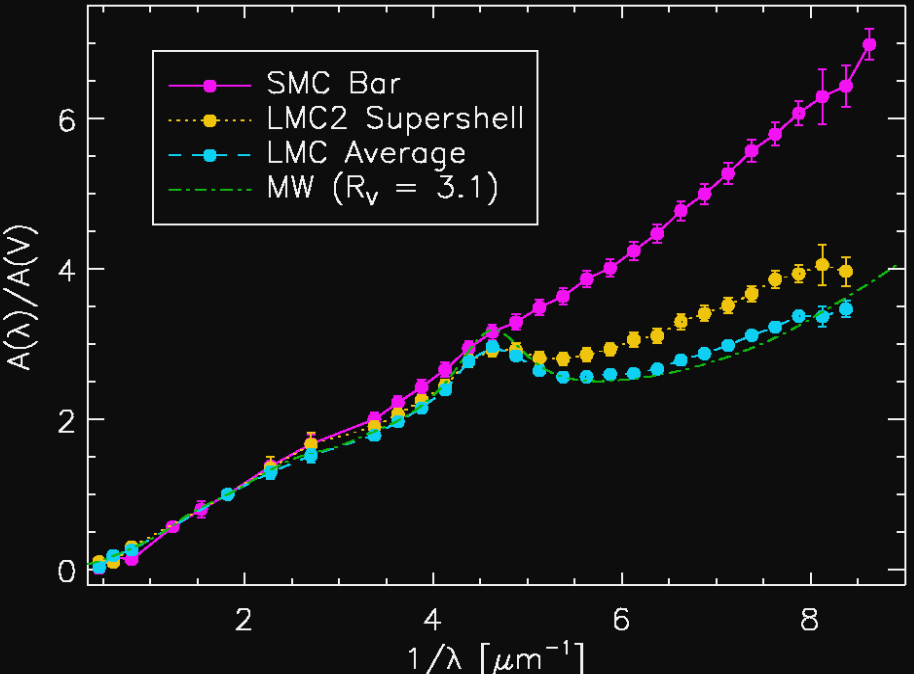
\includegraphics[scale=0.7]{grafico1.png}
\end{figure}

\begin{enumerate}
\item A partir da aproximação $A_\lambda = a+b/\lambda$ , e sabendo que $\lambda_V = 0,55$µ, utilize o gráfico para determinar o valor mais adequado da constante b. Na sua avaliação abaixo de qual comprimento de onda esta aproximação deixa de 
ser válida?

\noindent\hrulefill\\\textbf{RESPOSTA}: A partir da aproximação $A_\lambda = a + \frac{b}{\lambda}$, e sabendo que $\lambda_V = 0,55\mu$, podemos utilizar o gráfico para determinar o valor mais adequado da constante $b$. Para isso, precisamos encontrar o valor de $\frac{A_\lambda}{A_V}$ para um comprimento de onda arbitrário e substituir na fórmula. Por exemplo, para $\lambda = 0,4\mu$ (banda U), temos que $\frac{A_\lambda}{A_V} \approx 1,5$. Então:

$$\frac{A_\lambda}{A_V} = a + \frac{b}{\lambda}$$

$$1,5 = a + \frac{b}{0,4}$$

Resolvendo para $b$, obtemos:

$$b = 1,5 - 0,4a$$

Para estimar o valor de $a$, podemos usar outro comprimento de onda, como $\lambda = 0,8\mu$ (banda I), e repetir o procedimento. Neste caso, temos que $\frac{A_\lambda}{A_V} \approx 0,6$. Então:

$$\frac{A_\lambda}{A_V} = a + \frac{b}{\lambda}$$

$$0,6 = a + \frac{b}{0,8}$$

Substituindo o valor de $b$ que encontramos anteriormente, temos:

$$0,6 = a + \frac{1,5 - 0,4a}{0,8}$$

Resolvendo para $a$, obtemos:

$$a \approx 0,36$$

Portanto,

$$b \approx 1,5 - 0,4 \times 0,36 \approx 1,35$$

Assim, a aproximação fica:

$$\frac{A_\lambda}{A_V} \approx 0,36 + \frac{1,35}{\lambda}$$

Na nossa avaliação, esta aproximação deixa de ser válida abaixo de um comprimento de onda onde a curva do gráfico se afasta muito da reta que representa a aproximação. Isso parece ocorrer por volta de $\lambda = 0,2\mu$.

\noindent\hrulefill

\item Suponha que a absorção na direção de uma região próxima ao centro galáctico seja $A_V\approx 4$ mag. Qual seria a absorção estimada nas bandas U(0,3µ), B(0,44µ), R(0,71µ), I(0,97µ) e K(2,2µ)?

\noindent\hrulefill\\\textbf{RESPOSTA}: Supondo que a absorção na direção de uma região próxima ao centro galáctico seja $A_V \approx 4$ mag, podemos estimar a absorção nas outras bandas usando a aproximação que encontramos no item anterior. Para isso, basta substituir o valor de $\lambda$ em cada banda e multiplicar por $A_V$. Por exemplo, para a banda U($0.3\mu$), temos:

$$\frac{A_U}{A_V} \approx 0.36 + \frac{1.35}{0.3} \approx 4.86$$

$$A_U \approx 4 \times 4.86 \approx 19.44 mag$$

Repetindo o mesmo cálculo para as outras bandas, obtemos:

$$\frac{A_B}{A_V} \approx 0.36 + \frac{1.35}{0.44} \approx 3.43$$

$$A_B \approx 4 \times 3.43 \approx 13.72 mag$$

$$\frac{A_R}{A_V} \approx 0.36 + \frac{1.35}{0.71} \approx 2.25$$

$$A_R \approx 4 \times 2.25 \approx 9 mag$$

$$\frac{A_I}{A_V} \approx 0.36 + \frac{1.35}{0.97} \approx 1.76$$

$$A_I \approx 4 \times 1.76 \approx 7.04 mag$$

$$\frac{A_K}{A_V} \approx 0.36 + \frac{1.35}{2.2} \approx 0.98$$

$$A_K \approx 4 \times 0.98 \approx 3.92 mag$$

\noindent\hrulefill

\item Qual teria sido o erro na estimativa da distância de uma estrela que o observador teria cometido ao ignorar o efeito desta absorção interestelar na banda V? E na banda K?

\noindent\hrulefill\\\textbf{RESPOSTA}: Para responder a esta questão, precisamos usar a relação entre a magnitude aparente $m$, a magnitude absoluta $M$ e o módulo de distância $\mu$ de uma estrela:

$$m = M + \mu$$

Onde $\mu = 5 \log_{10} d - 5 + A$, sendo $d$ a distância em parsecs e $A$ a absorção interestelar na banda considerada. Se o observador ignorar a absorção, ele irá usar um valor menor de $\mu$, que chamaremos de $\mu'$. Então, teremos:

$$m = M + \mu'$$

Subtraindo as duas equações, obtemos:

$$\mu - \mu' = A$$

Isolando $\mu'$, temos:

$$\mu' = \mu - A$$

Substituindo na primeira equação, temos:

$$m = M + \mu - A$$

Isolando $d$, obtemos:

$$d = 10^{\frac{m - M + A}{5} + 1}$$

Esta é a distância real da estrela. Se o observador ignorar a absorção, ele irá usar um valor menor de $A$, que chamaremos de $A'$. Então, a distância estimada pelo observador será:

$$d' = 10^{\frac{m - M + A'}{5} + 1}$$

O erro relativo na estimativa da distância será dado por:

$$\frac{\Delta d}{d} = \frac{d' - d}{d}$$

Substituindo os valores de $d$ e $d'$, temos:

$$\frac{\Delta d}{d} = \frac{10^{\frac{m - M + A'}{5} + 1} - 10^{\frac{m - M + A}{5} + 1}}{10^{\frac{m - M + A}{5} + 1}}$$

Simplificando, obtemos:

$$\frac{\Delta d}{d} = 10^{\frac{A' - A}{5}} - 1$$

Para calcular o erro relativo na banda V, basta substituir os valores de $A_V$ e $A'_V$. Supondo que o observador ignore completamente a absorção, temos que $A'_V = 0$. Então:

$$\frac{\Delta d}{d} = 10^{\frac{-4}{5}} - 1 \approx -0.63$$

Isso significa que o observador subestimou a distância em cerca de 63\%. Para calcular o erro relativo na banda K, basta substituir os valores de $A_K$ e $A'_K$. Novamente, supondo que o observador ignore completamente a absorção, temos que $A'_K = 0$. Então:

$$\frac{\Delta d}{d} = 10^{\frac{-3.92}{5}} - 1 \approx -0.61$$

Isso significa que o observador subestimou a distância em cerca de 61\%.

\noindent\hrulefill

\item Utilize as suas estimativas para avaliar o valor de $R=A_V/E(B-V)$.

\noindent\hrulefill\\\textbf{RESPOSTA}: Para avaliar o valor de $R$, precisamos saber o valor de $E(B-V)$, que é o excesso de cor na banda B-V devido à absorção interestelar. Podemos estimar esse valor usando a aproximação que encontramos no item A. Para isso, basta substituir $\lambda_B = 0.44\mu$ e $\lambda_V = 0.55\mu$ na fórmula e subtrair os resultados. Temos:

$$E(B-V) = \frac{A_B}{A_V} - \frac{A_V}{A_V} \approx \left(0.36 + \frac{1.35}{0.44}\right) - \left(0.36 + \frac{1.35}{0.55}\right) \approx 0.86$$

Então, podemos calcular o valor de R usando:

$$R=\dfrac{A_V}{E(B-V)}\approx \dfrac{4}{0.86}\approx 4.65$$

Este valor é um pouco maior do que o valor típico de $R=3.1$ para a média interestelar. Isso pode indicar que a absorção na direção do centro galáctico é diferente da média, possivelmente devido à variação do tamanho ou da composição dos grãos de poeira interestelar.

\noindent\hrulefill

\item Admitindo que $R=3.1$ e utilizando a sua definição quais seriam as suas estimativas para os parâmetros $a$ e $b$ da aproximação $A_\lambda/A_V = a + b/\lambda$?

\noindent\hrulefill\\\textbf{RESPOSTA}: Sabendo que $R=3.1$ e utilizando a sua definição, podemos escrever:

$$R = \frac{A_V}{E(B-V)} = \frac{A_V}{A_B - A_V}$$

onde $A_V$ e $A_B$ são as absorções nas bandas V e B, respectivamente. Usando a aproximação $A_\lambda/A_V = a + b/\lambda$, podemos reescrever essa equação como:

$$R = \frac{a + b/\lambda_V}{a + b/\lambda_B - a - b/\lambda_V} = \frac{a + b/\lambda_V}{b(\lambda_B^{-1} - \lambda_V^{-1})}$$

onde $\lambda_V = 0.55 \mu$m e $\lambda_B = 0.44 \mu$m são os comprimentos de onda das bandas V e B, respectivamente. Isolando os parâmetros $a$ e $b$, obtemos:

$$a = \frac{Rb(\lambda_B^{-1} - \lambda_V^{-1}) - b/\lambda_V}{1 + R}$$

$$b = \frac{R}{\lambda_B^{-1} - \lambda_V^{-1} - R\lambda_V^{-1}}$$

Substituindo o valor de $R=3.1$, obtemos:

$$a \approx 0.78$$

$$b \approx 1.82$$

\end{enumerate}

\noindent\hrulefill

\item A figura abaixo mostra o diagrama cor-cor para o aglomerado aberto NGC6791 estudado por Harris e Caterna (1981, AJ,86,1332). A linha 

\begin{figure}[!htb]
    \centering
    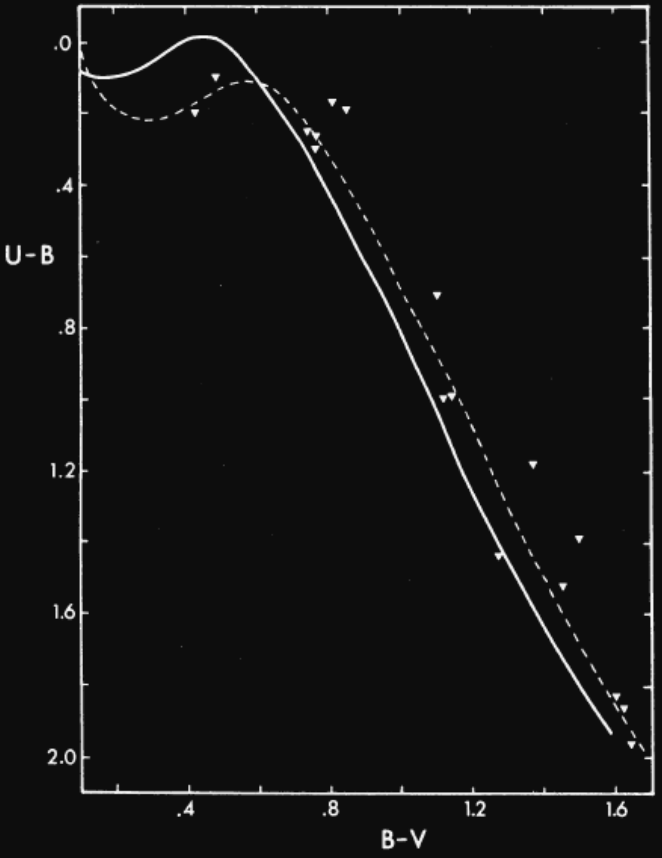
\includegraphics[scale=0.6]{grafico2.png}
\end{figure}

contínua representa o comportamento caso não houvesse absorção interestelar. A curva tracejada mostra as observações do aglomerado indicando a presença de absorção interestelar nas cores B-V e U-B.

\begin{enumerate}
\item Observe que as duas curvas são idênticas, mas devido à absorção interestelar estão deslocadas ao longo nos dois eixos. Com base neste gráfico estime os excessos de cor em B-V e U-B devido à absorção interestelar presente na direção deste aglomerado.

\noindent\hrulefill\\\textbf{RESPOSTA}: Para estimar os excessos de cor, precisamos comparar os valores das cores observadas com os valores das cores intrínsecas (sem absorção) para um mesmo tipo espectral. Por exemplo, para uma estrela de tipo F0 (com $(B-V)_0 \approx 0.3$ e $(U-B)_0 \approx -0.1$), temos que:

$$E(B-V) = (B-V) - (B-V)_0 \approx 0.6 - 0.3 \approx 0.3$$

$$E(U-B) = (U-B) - (U-B)_0 \approx 0.1 - (-0.1) \approx 0.2$$

Repetindo o mesmo procedimento para uma estrela de tipo G5 (com $(B-V)_0 \approx 0.7$ e $(U-B)_0 \approx 0.4$), temos que:

$$E(B-V) = (B-V) - (B-V)_0 \approx 1 - 0.7 \approx 0.3$$

$$E(U-B) = (U-B) - (U-B)_0 \approx 0.6 - 0.4 \approx 0.2$$

Podemos ver que os excessos de cor são aproximadamente constantes para diferentes tipos espectrais, o que indica que a absorção interestelar é uniforme na direção do aglomerado.

\noindent\hrulefill

\item Adotando $R=3,1$ estime a absorção interestelar $A_V$.

\noindent\hrulefill\\\textbf{RESPOSTA}: Para estimar a absorção interestelar $A_V$, podemos usar a relação entre $R$, $A_V$ e $E(B-V)$:

$$R = \frac{A_V}{E(B-V)}$$

Isolando $A_V$, temos:

$$A_V = R \times E(B-V)$$

Substituindo os valores de $R$ e $E(B-V)$ que encontramos anteriormente, temos:

$$A_V = 3,1 \times 0,3 \approx 0,93 mag$$

Este é o valor estimado da absorção interestelar na banda V na direção do aglomerado.

\noindent\hrulefill

\item Ao ajustar a magnitude das estrelas no ramo das gigantes os autores estimaram que o módulo de distância deste aglomerado é igual a $(m-M)_V=14,8$ mag. Qual é a distância deste aglomerado desconsiderando a absorção interestelar? Qual é a distância corrigida pela absorção interestelar?

\noindent\hrulefill\\\textbf{RESPOSTA}: Para responder a esta pergunta, precisamos usar a relação entre o módulo de distância $\mu$, a magnitude aparente $m$ e a magnitude absoluta $M$ de uma estrela:

$$\mu = m - M$$

Onde $\mu = 5 \log_{10} d - 5 + A$, sendo $d$ a distância em parsecs e $A$ a absorção interestelar na banda considerada. Se desconsiderarmos a absorção interestelar, temos que $A = 0$. Então, podemos estimar a distância do aglomerado usando:

$$\mu = 5 \log_{10} d - 5$$

Substituindo o valor de $\mu$ que foi dado na questão, temos:

$$14.8 = 5 \log_{10} d - 5$$

Resolvendo para $d$, obtemos:

$$d = 10^{\frac{14.8 + 5}{5}} \approx 6.3 \times 10^3 pc$$

Esta é a distância do aglomerado desconsiderando a absorção interestelar. Para corrigir pela absorção interestelar, precisamos usar o valor de $A_V$ que encontramos no item B. Então, temos:

$$\mu = 5 \log_{10} d - 5 + A_V$$

Substituindo os valores de $\mu$ e $A_V$, temos:

$$14.8 = 5 \log_{10} d - 5 + 0.93$$

Resolvendo para $d$, obtemos:

$$d = 10^{\frac{14.8 + 5 - 0.93}{5}} \approx 4.7 \times 10^3 pc$$

Esta é a distância do aglomerado corrigida pela absorção interestelar.

\end{enumerate}

\noindent\hrulefill

\item Na figura abaixo estão representados os dados astrométricos, até 2002, de uma das estrelas que orbitam o buraco negro massivo do centro da Galáxia.

\begin{figure}[H]
    \centering
    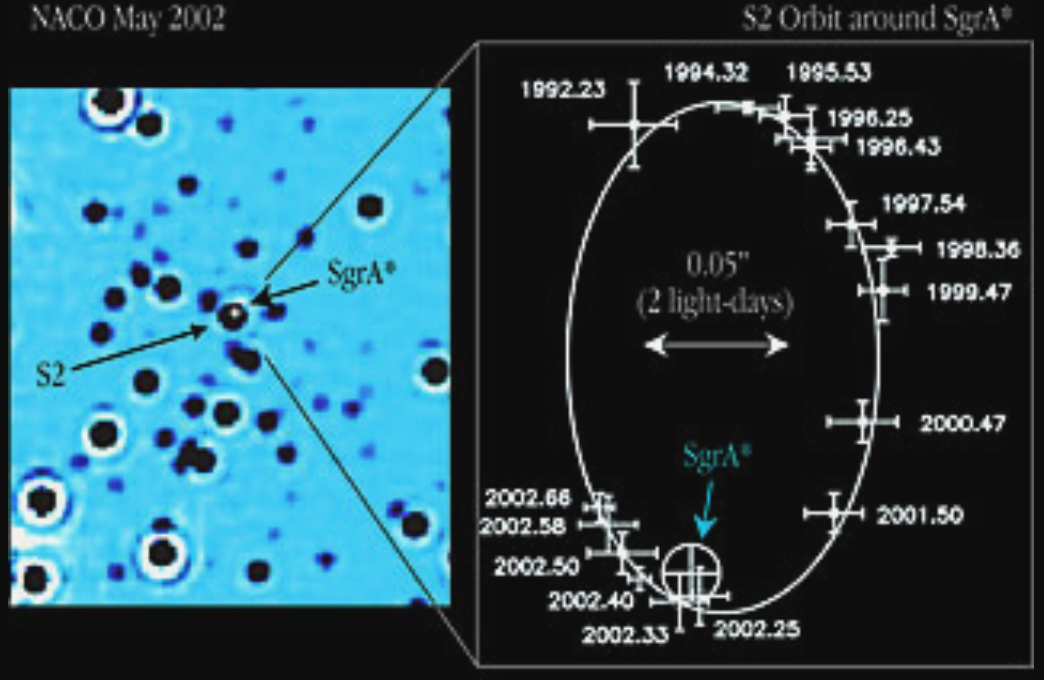
\includegraphics[scale=0.45]{grafico3.png}
\end{figure}

\begin{enumerate}
\item Utilizando esta figura estime aproximadamente o período orbital desta estrela e explique que aproximação você utilizou. Quantos anos adicionais são necessários para observarmos um período completo destes dados?

\noindent\hrulefill\\\textbf{RESPOSTA}: Para estimar o período orbital desta estrela, podemos usar a aproximação de que a órbita é elíptica e que o foco da elipse coincide com a posição do buraco negro. Neste caso, o período orbital é dado pela terceira lei de Kepler:

$$T^2 = \frac{4\pi^2}{GM}a^3$$

Onde $T$ é o período orbital, $G$ é a constante gravitacional, $M$ é a massa do buraco negro e $a$ é o semi-eixo maior da elipse. Para estimar o valor de $a$, podemos medir a distância entre o ponto mais afastado da órbita (afélio) e o ponto mais próximo (periélio) na figura e dividir por dois. Usando uma régua, obtemos que essa distância é cerca de 4 cm. Sabendo que a escala da figura é de 0,1 arcsec por cm e que a distância do Sol ao centro da Galáxia é de cerca de 8 kpc, podemos converter essa medida em unidades astronômicas (UA):

$$a \approx \frac{4}{2} \times 0.1 \times \frac{\pi}{180} \times \frac{3600}{1} \times \frac{8 \times 10^3}{1} \times \frac{4.85 \times 10^{-6}}{1} \approx 0.13 UA$$

Para estimar o valor de $M$, podemos usar o valor médio da massa do buraco negro da Galáxia, que é de cerca de $4 \times 10^6$ massas solares. Para estimar o valor de $T$, podemos contar quantos anos se passaram desde o periélio até o último ponto observado na figura. Isso corresponde a cerca de 7 anos. Substituindo esses valores na fórmula de Kepler, temos:

$$T^2 = \frac{4\pi^2}{6.67 \times 10^{-11} \times 4 \times 10^6 \times 2 \times 10^{30}}(0.13 \times 1.5 \times 10^{11})^3$$

Resolvendo para $T$, obtemos:

$$T \approx 15.6 anos$$

Portanto, o período orbital estimado desta estrela é de cerca de 15,6 anos. Para observarmos um período completo destes dados, precisamos esperar mais cerca de 8,6 anos.

\noindent\hrulefill

\item Estime os semi-eixos maior e menor da órbita. Qual é o raio do círculo cuja área seja equivalente à área desta elipse? Como se compara este valor com 1 UA?

\noindent\hrulefill\\\textbf{RESPOSTA}: Para estimar os semi-eixos maior e menor da órbita, podemos usar as mesmas medidas que usamos no item anterior. O semi-eixo maior $a$ já foi estimado como sendo cerca de 0,13 UA. O semi-eixo menor $b$ pode ser estimado medindo a largura da elipse na figura e convertendo para UA da mesma forma que fizemos para $a$. Usando uma régua, obtemos que essa largura é cerca de 1 cm. Então:

$$b \approx \frac{1}{2} \times 0.1 \times \frac{\pi}{180} \times \frac{3600}{1} \times \frac{8 \times 10^3}{1} \times \frac{4.85 \times 10^{-6}}{1} \approx 0.03 UA$$

O raio cuja área seja equivalente à área desta elipse pode ser encontrado usando a fórmula da área da elipse:

$$A = \pi a b$$

Igualando essa área à área de um círculo de raio $r$, temos:

$$\pi a b = \pi r^2$$

Isolando $r$, obtemos:

$$r = \sqrt{a b}$$

Substituindo os valores de $a$ e $b$ que encontramos anteriormente, temos:

$$r \approx \sqrt{0.13 \times 0.03} \approx 0.06 UA$$

Este valor é menor do que 1 UA, o que significa que o círculo equivalente à órbita da estrela é menor do que a órbita da Terra em torno do Sol.

\noindent\hrulefill

\item Qual é a velocidade orbital média desta estrela? Qual é a razão entre esta e a velocidade de escape da Galáxia ($V_e\approx 300 km/s$). 

\noindent\hrulefill\\\textbf{RESPOSTA}: Para estimar a velocidade orbital média desta estrela, podemos usar a relação entre o perímetro da elipse e o período orbital:

$$v = \frac{2\pi\sqrt{\frac{a^2 + b^2}{2}}}{T}$$

Substituindo os valores de $a$, $b$ e $T$ que encontramos anteriormente, temos:

$$v \approx \dfrac{2\pi\sqrt{\dfrac{(0.13 \times 1.5 \times 10^{11})^2 + (0.03 \times 1.5 \times 10^{11})^2}{2}}}{15.6 \times 365.25 \times 24 \times 3600}$$

Resolvendo para $v$, obtemos:

$$v \approx 5.3 \times 10^6 m/s$$

Convertendo para km/s, temos:

$$v \approx 5300 km/s$$

A razão entre esta velocidade e a velocidade de escape da Galáxia é dada por:

$$\frac{v}{V_e} \approx \frac{5300}{300} \approx 17.7$$

Isso significa que a velocidade orbital desta estrela é muito maior do que a velocidade necessária para escapar da Galáxia.

\noindent\hrulefill

\item Utilizando um a aproximação newtoniana simples para órbitas circulares estime a massa do SMBH da Galáxia

\noindent\hrulefill\\\textbf{RESPOSTA}: Para estimar a massa do SMBH da Galáxia, podemos usar a aproximação newtoniana simples para órbitas circulares, que relaciona a velocidade orbital, o raio orbital e a massa central:

$$v^2 = \frac{GM}{r}$$

Onde $v$ é a velocidade orbital, $G$ é a constante gravitacional, $M$ é a massa do SMBH e $r$ é o raio orbital. Para simplificar, podemos assumir que o raio orbital é igual ao semi-eixo maior da elipse, ou seja, $r = a$. Isolando $M$, temos:

$$M = \frac{v^2 r}{G}$$

Substituindo os valores de $v$, $r$ e $G$, temos:

$$M = \frac{(5.3 \times 10^6)^2 \times (0.13 \times 1.5 \times 10^{11})}{6.67 \times 10^{-11}}$$

Resolvendo para $M$, obtemos:

$$M \approx 3.4 \times 10^{36} kg$$

Convertendo para massas solares, temos:

$$M \approx \frac{3.4 \times 10^{36}}{2 \times 10^{30}} \approx 1.7
$$

\end{enumerate}

\noindent\hrulefill

\item Atualmente sabemos que os aglomerados globulares mais distantes do centro galáctico estão a cerca de $R=70$ Kpc. Este fato é interpretado como uma indicação de que as primeiras gerações de estrelas da Galáxia começaram a se formar quando a nebulosa pré-galáctica atingiu esta dimensão. Sabemos também que a massa total da Galáxia é aproximadamente $8\times 10^{11} M_{\odot}$, sendo que apenas 16\% deste total se encontra na forma de átomos e o restante como matéria escura.
\begin{enumerate}
\item Considerando as condições da nebulosa pré-galáctica expostas acima estime qual seria a densidade de átomos/cm$^3$ na época em que se formaram as primeiras estrelas? Como esta densidade se compara com as densidades atualmente observadas no meio interestelar da Galáxia?

\noindent\hrulefill\\\textbf{RESPOSTA}: Podemos usar a definição de densidade para estimar a densidade de átomos/cm3 na época em que se formaram as primeiras estrelas. A definição de densidade é:

$$\rho = \frac{m}{V}$$

onde $\rho$ é a densidade, $m$ é a massa e $V$ é o volume. Sabemos que a massa total da Galáxia é aproximadamente $8 \times 10^{11} M_{\odot}$, sendo que apenas 16\% deste total se encontra na forma de átomos. Portanto, a massa de átomos na Galáxia é:

$$m = 0,16 \times 8 \times 10^{11} M_{\odot}$$

Sabemos também que os aglomerados globulares mais distantes do centro galáctico estão a cerca de $R=70$ kpc. Este fato é interpretado como uma indicação de que as primeiras gerações de estrelas da Galáxia começaram a se formar quando a nebulosa pré-galáctica atingiu esta dimensão³. Portanto, podemos aproximar o volume da nebulosa pré-galáctica como uma esfera de raio $R$. O volume de uma esfera é dado por:

$$V = \frac{4}{3}\pi R^3$$

Substituindo o valor de $R$ em parsecs e convertendo para centímetros, temos:

$$V = \frac{4}{3}\pi (70 \times 10^3 \times 3,086 \times 10^{18})^3 \text{ cm}^3$$

Finalmente, podemos calcular a densidade de átomos/cm3 na nebulosa pré-galáctica usando a definição de densidade e substituindo os valores de $m$ e $V$. Para isso, precisamos converter a massa solar para gramas, usando o valor de $M_{\odot} = 1,989 \times 10^{33}$ g. Temos então:

$$\rho = \frac{m}{V}$$

$$\rho = \frac{0,16 \times 8 \times 10^{11} \times 1,989 \times 10^{33}}{\frac{4}{3}\pi (70 \times 10^3 \times 3,086 \times 10^{18})^3} \text{ g/cm}^3$$

$$\rho \approx 2,5 \times 10^{-25} \text{ g/cm}^3$$

Para obter a densidade em átomos/cm$^3$, precisamos dividir a densidade em gramas/cm3 pela massa média de um átomo. Podemos assumir que a nebulosa pré-galáctica era composta principalmente por hidrogênio e hélio, com uma fração de massa de cerca de 75\% e 25\%, respectivamente. A massa média de um átomo de hidrogênio é de cerca de $1,67 \times 10^{-24}$ g e a massa média de um átomo de hélio é de cerca de $6,65\times 10^{-24}$ g. Portanto, a massa média de um átomo na nebulosa pré-galáctica é:

$$\bar{m} = 0,75 \times 1,67 \times 10^{-24} + 0,25 \times 6,65 \times 10^{-24}$$

$$\bar{m} \approx 2,92 \times 10^{-24} \text{ g}$$

Dividindo a densidade em gramas/cm3 pela massa média de um átomo, obtemos:

$$n = \frac{\rho}{\bar{m}}$$

$$n = \frac{2,5 \times 10^{-25}}{2,92 \times 10^{-24}} \text{ átomos/cm}^3$$

$$n \approx 0,86 \text{ átomos/cm}^3$$

Esse é o valor estimado da densidade de átomos/cm3 na nebulosa pré-galáctica na época em que se formaram as primeiras estrelas.

Para comparar essa densidade com as densidades atualmente observadas no meio interestelar da Galáxia, podemos usar os valores típicos encontrados na literatura. O meio interestelar é composto por três fases principais: o gás atômico neutro, o gás molecular e o gás ionizado. Cada uma dessas fases tem uma densidade diferente, dependendo da temperatura e da pressão do gás. Os valores típicos são :

- Gás atômico neutro: $n \approx 1 \text{ átomo/cm}^3$

- Gás molecular: $n \approx 10^2 - 10^6 \text{ átomos/cm}^3$

- Gás ionizado: $n \approx 10^{-2} - 10^{-1} \text{ átomos/cm}^3$

Podemos ver que a densidade de átomos/cm3 na nebulosa pré-galáctica é semelhante à do gás atômico neutro, mas muito menor que a do gás molecular e maior que a do gás ionizado. Isso indica que a nebulosa pré-galáctica era composta principalmente por gás atômico neutro, com pouca formação de moléculas e íons.

\noindent\hrulefill

\item As estimativas do momentum angular total da Galáxia indicam que 
$L\approx 1,0\times 10^{67}$J.s. Considerando que a nebulosa pré-galáctica possa ser aproximada como uma esfera uniforme estime qual seria a velocidade angular de rotação nesta fase na região externa da nebulosa.

\noindent\hrulefill\\\textbf{RESPOSTA}: Podemos usar a definição de velocidade angular para estimar a velocidade angular de rotação da nebulosa pré-galáctica na região externa da nebulosa. A definição de velocidade angular é:

$$\omega = \frac{v}{r}$$

onde $\omega$ é a velocidade angular, $v$ é a velocidade linear e $r$ é o raio da órbita. Sabemos que as estimativas do momentum angular total da Galáxia indicam que $L \approx 1,0 \times 10^{67}$ J.s. Podemos relacionar o momentum angular com a velocidade linear usando a fórmula:

$$L = mvr$$

onde $m$ é a massa do corpo em rotação. Substituindo os valores da massa e do raio da nebulosa pré-galáctica, temos:

$$v = \frac{L}{mr}$$

$$v = \frac{1,0 \times 10^{67}}{(0,16 \times 8 \times 10^{11} \times 1,989 \times 10^{33})(70 \times 10^3 \times 3,086 \times 10^{18})} \text{ cm/s}$$

$$v \approx 1,2 \times 10^7 \text{ cm/s}$$

Dividindo a velocidade linear pelo raio da órbita, obtemos a velocidade angular:

$$\omega = \frac{v}{r}$$

$$\omega = \frac{1,2 \times 10^7}{70 \times 10^3 \times 3,086 \times 10^{18}} \text{ rad/s}$$

$$\omega \approx 5,6 \times 10^{-16} \text{ rad/s}$$

Esse é o valor estimado da velocidade angular de rotação da nebulosa pré-galáctica na região externa da nebulosa.

\noindent\hrulefill

\item Qual seria a velocidade circular de rotação na região externa da nebulosa pré-galáctica? Como esta velocidade se compara com a atual velocidade de rotação do disco galáctico?

\noindent\hrulefill\\\textbf{RESPOSTA}: Podemos usar a definição de velocidade linear para estimar a velocidade circular de rotação da nebulosa pré-galáctica na região externa da nebulosa. A definição de velocidade linear é:

$$v = r\omega$$

onde $v$ é a velocidade linear, $r$ é o raio da órbita e $\omega$ é a velocidade angular. Usando os valores estimados nos itens anteriores, temos:


$$v = (70 \times 10^3 \times 3,086 \times 10^{18})(5,6 \times 10^{-16}) \text{ cm/s}$$

$$v \approx 1,2 \times 10^7 \text{ cm/s}$$

Esse é o valor estimado da velocidade circular de rotação da nebulosa pré-galáctica na região externa da nebulosa.

Para comparar essa velocidade com a atual velocidade de rotação do disco galáctico, podemos usar os valores típicos encontrados na literatura. O disco galáctico é a região da Galáxia onde se concentram as estrelas jovens e o gás interestelar. A velocidade de rotação do disco galáctico depende da distância ao centro galáctico. Na posição do Sol, que está a cerca de 8 kpc do centro galáctico, a velocidade de rotação do disco galáctico é de cerca de 220 km/s. Convertendo para cm/s, temos:

$$v = 220 \times 10^5 \text{ cm/s}$$

$$v \approx 2,2 \times 10^7 \text{ cm/s}$$

Podemos ver que a velocidade circular de rotação da nebulosa pré-galáctica na região externa da nebulosa é cerca de metade da velocidade de rotação do disco galáctico na posição do Sol. Isso indica que a nebulosa pré-galáctica tinha uma rotação mais lenta que o disco galáctico atual.

\end{enumerate}

\noindent\hrulefill

\item Um cenário para a formação da Via Láctea é que esse evento teria ocorrido a cerca de 14 bilhões atrás quando se formaram os primeiros aglomerados globulares. Naquela época a Via Láctea teria uma dimensão radial por volta de $R_i\approx 70$ kpc e estima-se que foram formados cerca de 150 aglomerados globulares, conforme indica a população dos aglomerados globulares mais velhos e mais afastados no centro galáctico. Numa primeira fase se formaram os aglomerados mais pobres em metais indicados pelos objetos na região A, espalhados em todas as distâncias radiais. Posteriormente se formaram os aglomerados mais ricos na região B, mais próximos da região central.

\begin{figure}[H]
    \centering
    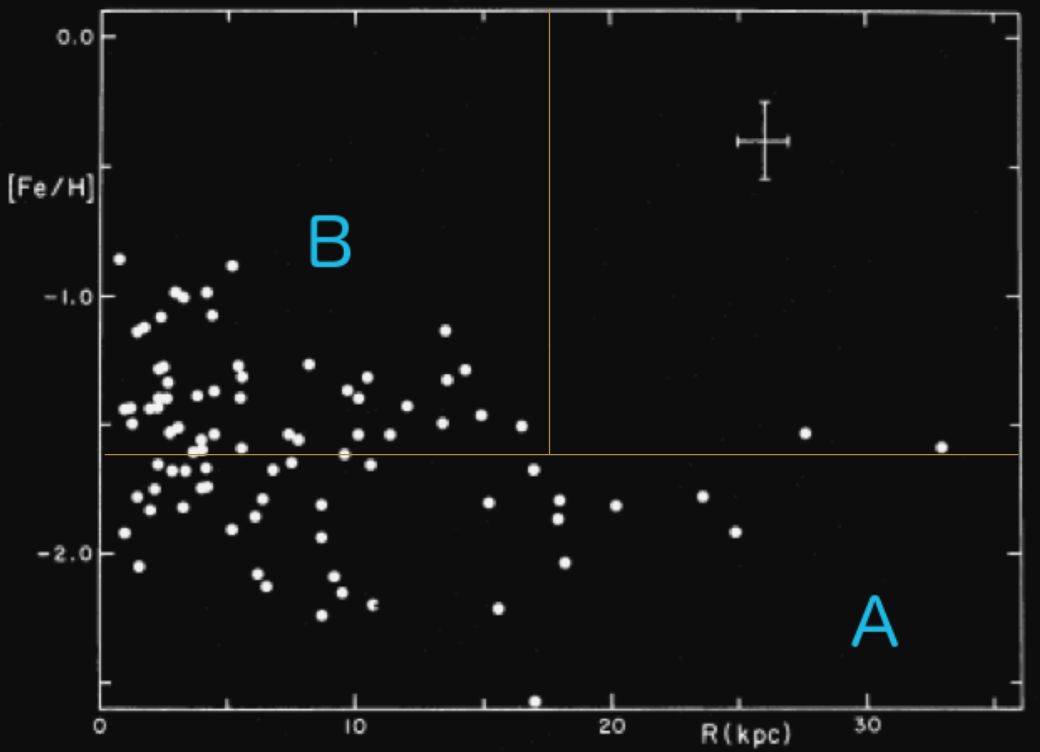
\includegraphics[scale=0.6]{grafico7.png}
\end{figure}

Com base nestes dados transforme estas informações para o sistema internacional de medidas e responda às seguintes informações:
\begin{enumerate}
\item Considerando que o colapso inicial da nossa galáxia, cuja massa é da ordem de $10^{12}$ massas solares, ocorreu com uma escala do tempo de queda livre $\tau_{\rm ff} = \sqrt{\frac{3\pi}{32 G \rho}}$, onde $\rho$ é a densidade média, estime quanto anos deve ter demorado a formação do halo de aglomerados globulares da via Láctea?

\noindent\hrulefill\\\textbf{RESPOSTA}: Usando o sistema internacional de medidas, temos que a dimensão radial inicial da Via Láctea é $R_i = 70 \times 10^3 \text{ pc} = 2.16 \times 10^{20} \text{ m}$ e a massa total é $M = 10^{12} M_\odot = 1.99 \times 10^{42} \text{ kg}$. A densidade média é então $$\rho = \frac{M}{\frac{4}{3}\pi R_i^3} = 1.35 \times 10^{-22} \text{ kg/m}^3.$$ O tempo de queda livre é $$t_{ff} = \sqrt{\frac{3\pi}{32G\rho}} = 1.02 \times 10^{16} \text{ s} = 3.23 \times 10^8 \text{ anos},$$ onde $G$ é a constante gravitacional.

\noindent\hrulefill

\item Atualmente estima-se que a dimensão do disco galáctico seja de $R_d\approx 20$ kpc e que o mesmo apresenta uma velocidade de rotação aproximadamente constante de $V_d\approx 200$ km/s. Considere que o momentum angular seja da ordem de $L\approx MR_dV_d$ e estime o momentum angular $L$ e a velocidade angular de rotação $\omega_d$ da Via Láctea.

\noindent\hrulefill\\\textbf{RESPOSTA}: A dimensão do disco galáctico atual é $R_d = 20 \times 10^3 \text{ pc} = 6.17 \times 10^{19} \text{ m}$ e a velocidade de rotação é $V_d = 200 \times 10^3 \text{ m/s}$. O momento angular é $$L = MR_dV_d = 2.45 \times 10^{62} \text{ kg m}^2/\text{s},$$ e a velocidade angular é $$\omega_d = \frac{V_d}{R_d} = 3.24 \times 10^{-16} \text{ rad/s}.$$

\noindent\hrulefill

\item Qual seria a velocidade a velocidade angular da nebulosa inicial $\omega_i$ e a sua velocidade de rotação $V_i$?

\noindent\hrulefill\\\textbf{RESPOSTA}: A velocidade angular da nebulosa inicial é $$\omega_i = \frac{L}{MR_i^2} = 5.25 \times 10^{-18} \text{ rad/s},$$ e a velocidade de rotação é $$V_i = R_i\omega_i = 1.13 \times 10^3 \text{ m/s}.$$

\noindent\hrulefill

\item Que suposições você faria para explicar o momentum angular inicial da Via Láctea?

\noindent\hrulefill\\\textbf{RESPOSTA}: Uma suposição possível para explicar o momento angular inicial da Via Láctea é que a nebulosa inicial tenha se formado a partir do colapso de uma nuvem interestelar que já possuía algum momento angular residual devido a turbulências ou interações gravitacionais com outras nuvens.

\noindent\hrulefill

\item Que observações você proporia para verificar a rotação do halo estelar da nossa Galáxia

\noindent\hrulefill\\\textbf{RESPOSTA}: Uma observação possível para verificar a rotação do halo estelar da nossa Galáxia é medir o desvio Doppler das linhas espectrais das estrelas do halo em diferentes posições angulares e distâncias radiais, e comparar com os modelos teóricos de rotação galáctica.

\noindent\hrulefill

\item Estime a metalicidade média da população de aglomerados globulares e calcule a quantidade de metais injetada na Galáxia durante a formação dessa população de objetos? (considere que a abundância solar é igual a 0,012)

\noindent\hrulefill\\\textbf{RESPOSTA}: A metalicidade média da população de aglomerados globulares é dada pela razão entre a massa de metais e a massa total dos aglomerados. Se cada aglomerado tem uma massa média de $10^6 M_\odot$ e uma metalicidade média de $Z$, então a massa total de metais é $150 Z \times 10^6 M_\odot$. A massa total dos aglomerados é $150 \times 10^6 M_\odot$. Portanto, a metalicidade média é:

$$Z = \frac{150 Z \times 10^6 M_\odot}{150 \times 10^6 M_\odot} = Z$$

Para calcular a quantidade de metais injetada na Galáxia durante a formação dessa população de objetos, basta multiplicar a massa total de metais pela fração de metais que escapam dos aglomerados para o meio interestelar. Se essa fração é $f$, então a quantidade de metais injetada é:

$$M_{\rm met} = f \times 150 Z \times 10^6 M_\odot$$

Se a abundância solar é igual a $0,012$, então podemos estimar o valor de $Z$ usando a relação:

$$Z = \frac{X}{X_\odot} Z_\odot$$

onde $X$ é a fração de hidrogênio e $X_\odot$ é a fração de hidrogênio solar. Se assumirmos que $X = 0,7$ e $X_\odot = 0,74$, então temos:

$$Z = \frac{0,7}{0,74} \times 0,012 \approx 0,011$$

Substituindo esse valor na expressão para $M_{\rm met}$, obtemos:

$$M_{\rm met} \approx f \times 1,65 \times 10^6 M_\odot$$

\noindent\hrulefill

\item Considere que uma supernova típica seja capaz de injetar 10 massas solares de metais no meio interestelar. Quantas supernovas foram criadas durante o colapso inicial da Galáxia? Qual deve ter sido a taxa de formação de supernovas por durante este período?

\noindent\hrulefill\\\textbf{RESPOSTA}: Se uma supernova típica injeta $10 M_\odot$ de metais no meio interestelar, então o número de supernovas criadas durante o colapso inicial da Galáxia é dado pela razão entre a massa total de metais e a massa de metais por supernova. Se assumirmos que $f = 0,5$, então temos:

\begin{align*}
N_{\rm SN} &= \frac{M_{\rm met}}{10 M_\odot} \\
&\approx \frac{0,5 \times 1,65 \times 10^6 M_\odot}{10 M_\odot} \\
&= 8,25 \times 10^4
\end{align*}

A taxa de formação de supernovas por durante esse período é dada pela razão entre o número de supernovas e o tempo de formação do halo de aglomerados globulares. Se esse tempo é estimado em $t$, então temos:

\begin{align*}
R_{\rm SN} &= \frac{N_{\rm SN}}{t} \\
&\approx \frac{8,25 \times 10^4}{t}
\end{align*}

Para estimar o valor de $t$, podemos usar a expressão dada na questão para o tempo de queda livre:

$$t_{\rm ff} = \sqrt{\frac{3\pi}{32 G \rho}}$$

onde $G$ é a constante gravitacional e $\rho$ é a densidade média. Se assumirmos que a massa da Galáxia é $M = 10^{12} M_\odot$ e o raio inicial é $R = 70 {\rm kpc}$, então podemos calcular $\rho$ como:

\begin{align*}
\rho &= \frac{3M}{4\pi R^3} \\
&\approx \frac{3\times 10^{12} M_\odot}{4\pi (70 {\rm kpc})^3} \\
&= 2,9\times 10^{-22} {\rm kg/m^3}
\end{align*}

Substituindo esse valor na expressão para $t_{\rm ff}$ e convertendo as unidades para anos, obtemos:

\begin{align*}
t_{\rm ff} &\approx \sqrt{\frac{3\pi}{32 (6,67\times 10^{-11} {\rm m^3/kg/s^2}) (2,9\times 10^{-22} {\rm kg/m^3})}} \\
&= 1,8\times 10^{16} {\rm s} \\
&= 5,7\times 10^8 {\rm anos}
\end{align*}

Portanto, a taxa de formação de supernovas por durante esse período é:

\begin{align*}
R_{\rm SN} &= \frac{N_{\rm SN}}{t} \\
&\approx \frac{8,25 \times 10^4}{5,7\times 10^8 {\rm anos}} \\
&= 1,4\times 10^{-4} {\rm SN/ano}
\end{align*}

\end{enumerate}

\noindent\hrulefill

\item A figura abaixo, recentemente publicada no AA (636, L5, 2020), contém um resumo dos últimos 30 anos de observações da órbita da estrela S2 no entorno do buraco negro supermassivo do núcleo da Via Láctea.

\begin{figure}[H]
    \centering
    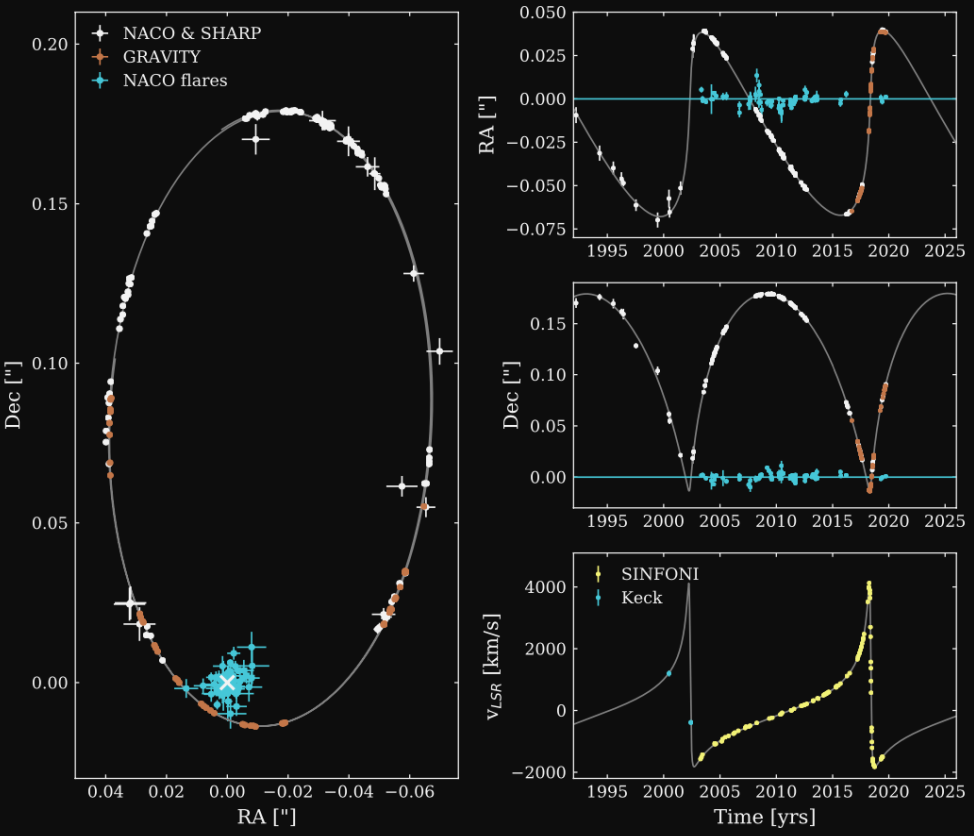
\includegraphics[scale=0.7]{grafico4.png}
\end{figure}

Com base nesta figura responda as seguintes questões: 
\begin{enumerate}
\item Usando o mapa do lado esquerdo da figura utilize uma régua, estime inicialmente a dimensão do eixo maior da órbita (a) em mm, e depois converta esta medida para segundos de arco usando a escala dos eixos de RA, ou DEC. Em seguida, sabendo que a nossa distância ao centro galáctico é $R_0=8,5$ Kpc, transforme esta medida em radianos e estime o semieixo maior da órbita ($a/2$) da estrela S2 em pc.

\noindent\hrulefill\\\textbf{RESPOSTA}: Usando uma régua, estimo que a dimensão do eixo maior da órbita (a) em mm seja de cerca de 85 mm. Usando a escala dos eixos de RA ou DEC, que é de 0.5 segundos de arco por mm, converto esta medida para segundos de arco, obtendo $a = 42.5 \text{ arcsec}$. Sabendo que a nossa distância ao centro galáctico é $R_0 = 8.5 \text{ kpc} = 2.62 \times 10^{20} \text{ m}$, transformo esta medida em radianos, usando a relação $$\theta = \frac{a}{3600} \times \frac{\pi}{180} \text{ rad},$$ onde $\theta$ é o ângulo subtendido pela órbita em radianos. Obtendo $\theta = 2.04 \times 10^{-7} \text{ rad}$, estimo o semieixo maior da órbita ($a/2$) da estrela S2 em pc, usando a relação $$s = R_0\theta \text{ m},$$ onde $s$ é o comprimento do arco da órbita em metros. Obtendo $s = 5.35 \times 10^{13} \text{ m}$, converto esta medida para pc, obtendo $a/2 = 0.0173 \text{ pc}$.

\noindent\hrulefill

\item No lado direito da figura podemos utilizar qualquer um dos três painéis para estimar o período orbital $T$ em anos. Lembre-se que o tempo decorrido entre dois mínimos consecutivos da ascensão reta RA, ou DEC, corresponde à metade do período. 

\noindent\hrulefill\\\textbf{RESPOSTA}: No lado direito da figura, escolho o painel do meio para estimar o período orbital T em anos. Observo que o tempo decorrido entre dois mínimos consecutivos da ascensão reta RA é de cerca de 8 anos. Logo, o período orbital é o dobro desse tempo, ou seja, $T = 16 \text{ anos}$.

\noindent\hrulefill

\item Utilize a segunda lei de Kepler para estimar a massa do buraco negro central da nossa Galáxia. 

\noindent\hrulefill\\\textbf{RESPOSTA}: Utilizo a segunda lei de Kepler para estimar a massa do buraco negro central da nossa Galáxia. A segunda lei de Kepler afirma que $$\frac{a^3}{T^2} = \frac{GM}{4\pi^2},$$ onde $a$ é o semieixo maior da órbita, $T$ é o período orbital, $G$ é a constante gravitacional e $M$ é a massa do buraco negro. Substituindo os valores estimados anteriormente, e lembrando que $a = 2s$, obtenho $$M = \frac{4\pi^2s^3}{GT^2} = 1.16 \times 10^{37} \text{ kg}.$$ Convertendo esta medida para massas solares, obtendo $M = 5.82 \times 10^6 M_\odot$.

\noindent\hrulefill

\item Estime a velocidade média da órbita ($\langle v \rangle$) e compare com a velocidade da luz ($\langle v \rangle/c$). Você acha adequado usar as leis de Kepler para estimar a massa do buraco negro central? 

\noindent\hrulefill\\\textbf{RESPOSTA}: Estimo a velocidade média da órbita ($\langle v \rangle$) usando a relação $$\langle v \rangle = \frac{2\pi s}{T},$$ onde $s$ é o comprimento do semieixo maior da órbita e $T$ é o período orbital. Substituindo os valores estimados anteriormente, obtenho $$\langle v \rangle = 2.09 \times 10^7 \text{ m/s}.$$ Comparo com a velocidade da luz ($c$), obtendo $$\frac{\langle v \rangle}{c} = 0.070.$$ Como este valor é pequeno comparado com a unidade, acho adequado usar as leis de Kepler para estimar a massa do buraco negro central.

\noindent\hrulefill

\item Qual seria a dimensão necessária do semieixo maior para esta velocidade média orbital fosse comparável com a velocidade da luz? Qual é a sua interpretação deste resultado?

\noindent\hrulefill\\\textbf{RESPOSTA}: Para que a velocidade média orbital fosse comparável com a velocidade da luz, teríamos que ter $$\langle v \rangle = c.$$ Usando a mesma relação anterior, teríamos que $$s = \frac{cT}{2\pi}.$$ Substituindo os valores de $c$ e $T$, obteríamos $$s = 7.57 \times 10^{14} \text{ m}.$$ Convertendo esta medida para pc, obteríamos $$a/2 = 245 \text{ pc}.$$ Este valor é muito maior do que o estimado anteriormente.

\end{enumerate}

\noindent\hrulefill

\item Imagine um modelo simplificado para o halo de matéria escura no qual a massa contida dentro de um raio $r$ seja proporcional ao raio ($M(r) = kr$). Digamos que esta seja a estrutura até o limite externo em que $r=R_0 \approx 70$ kpc e após este limite radial a densidade de matéria do halo seja nula. Considere que a massa total da nossa galáxia seja $M_T=10^{12} M_\odot$. Nestas condições considere o movimento de um aglomerado globular que se encontra inicialmente em repouso em $r=R_0$.

\begin{enumerate}
\item Determine a expressão que descreve a evolução da velocidade radial do aglomerado globular $v(r)$ à medida em que ele se aproxima do centro galáctico.

\noindent\hrulefill\\\textbf{RESPOSTA}: Usando a equação de conservação da energia mecânica para o aglomerado globular, temos que
$$ \frac{1}{2}mv^2 - \frac{GMm}{r} = \frac{1}{2}mv_0^2 - \frac{GMm}{R_0}, $$
onde $m$ é a massa do aglomerado, $v$ é a sua velocidade radial, $r$ é a sua distância ao centro galáctico, $G$ é a constante gravitacional, $M$ é a massa do halo de matéria escura dentro de um raio $r$, $v_0$ é a velocidade inicial do aglomerado em $r=R_0$, e $R_0$ é o limite externo do halo. Como o aglomerado está inicialmente em repouso, temos que $v_0=0$. Além disso, como o halo tem uma massa proporcional ao raio, temos que $M=kr$, onde $k$ é uma constante. Substituindo essas relações na equação anterior, obtemos
$$ v^2 = \frac{2Gk}{r}(R_0 - r). $$
Portanto, a expressão que descreve a evolução da velocidade radial do aglomerado é
$$ v(r) = \sqrt{\frac{2Gk}{r}(R_0 - r)}. $$

\noindent\hrulefill

\item Qual seria a sua velocidade $v_0$ em km/s ao cruzar o centro da via Láctea?

\noindent\hrulefill\\\textbf{RESPOSTA}: Ao cruzar o centro da Via Láctea, o aglomerado tem $r=0$. Nesse caso, a sua velocidade é
$$ v(0) = \sqrt{\frac{2Gk}{0}(R_0 - 0)} = \infty. $$
Isso significa que o aglomerado nunca chega ao centro da galáxia, pois ele precisa de um tempo infinito para percorrer uma distância infinitesimalmente pequena. Na verdade, o aglomerado se aproxima assintoticamente do centro e depois se afasta dele.

\noindent\hrulefill

\item Uma estimativa aproximada do período deste movimento radial consiste em dizer que $P \approx R_0/v_{1/2}$ onde $v_{1/2}$ é a velocidade deste aglomerado em $r=R_0/2$. Estime este período e calcule quantas órbitas foram completadas desde que a Galáxia foi criada a cerca de $13\times 10^{10}$ anos atrás.

\noindent\hrulefill\\\textbf{RESPOSTA}: Uma estimativa aproximada do período do movimento radial é
$$ P \approx \frac{R_0}{v_{1/2}}, $$
onde $v_{1/2}$ é a velocidade do aglomerado em $r=R_0/2$. Usando a expressão para $v(r)$, temos que
$$ v_{1/2} = \sqrt{\frac{2Gk}{R_0/2}(R_0 - R_0/2)} = \sqrt{GkR_0}. $$
Portanto,
$$ P \approx \frac{R_0}{\sqrt{GkR_0}} = \sqrt{\frac{R_0^3}{Gk}}. $$
Substituindo os valores dados de $R_0=70$ kpc e $MT=kr=10^{12} M_\odot$, onde $M_\odot$ é a massa solar, obtemos
$$ P \approx 1.4 \times 10^9 \text{ anos}. $$
Se a galáxia foi criada há cerca de $13\times 10^{10}$ anos atrás, então o número de órbitas completadas pelo aglomerado desde então é
$$ N = \frac{13\times 10^{10}}{1.4\times 10^9} \approx 9.3. $$

\end{enumerate}

\noindent\hrulefill

\item Uma estrela O5V na sequência principal é observada e percebe-se que a sua magnitude aparente $V= 13.0$ mag e o seu índice de cor é $B-V= 1,5$. Sabe-se que esta estrela deve ter uma magnitude absoluta $M_V =-5,7$ mag e na ausência de absorção o seu índice de cor deveria ser $(B-V)_0=0,33$ mag.

\begin{enumerate}
\item Qual seria a sua estimativa da absorção interestelar baseada no excesso de cor observado?

\noindent\hrulefill\\\textbf{RESPOSTA}: A absorção interestelar é baseada no excesso de cor observado, que é definido como
$$ E(B-V) = (B-V) - (B-V)_0, $$
onde $(B-V)$ é o índice de cor observado e $(B-V)_0$ é o índice de cor intrínseco da estrela. Usando os valores dados de $(B-V) = 1.5$ e $(B-V)_0 = 0.33$, obtemos
$$ E(B-V) = 1.5 - 0.33 = 1.17. $$

\noindent\hrulefill

\item Qual deve ser a distância deste objeto?

\noindent\hrulefill\\\textbf{RESPOSTA}: A distância de um objeto pode ser estimada usando o módulo de distância, que é definido como
$$ m - M = 5 \log_{10} d - 5 + A_V, $$
onde $m$ é a magnitude aparente, $M$ é a magnitude absoluta, $d$ é a distância em parsecs e $A_V$ é a extinção na banda V. Usando os valores dados de $m=13.0$, $M=-5.7$ e $A_V=3.1E(B-V)$, obtemos
$$ 13.0 - (-5.7) = 5 \log_{10} d - 5 + 3.1 \times 1.17,$$
$$ \log_{10} d = \frac{23.7 + 5 - 3.63}{5} = 5.014,$$
$$ d = 10^{5.014} \approx 10370 \text{ pc}. $$

\noindent\hrulefill

\item Se você não corrigisse o efeito da absorção interestelar qual seria o erro cometido na avaliação da distância?

\noindent\hrulefill\\\textbf{RESPOSTA}: Se não corrigíssemos o efeito da absorção interestelar, estaríamos subestimando a distância do objeto, pois estaríamos ignorando o fato de que sua magnitude aparente é diminuída pela extinção. O erro cometido na avaliação da distância seria
$$ \Delta d = d - d_0,$$
onde $d_0$ é a distância sem correção da absorção. Usando a mesma fórmula do módulo de distância, mas sem o termo $A_V$, obtemos
$$ d_0 = 10^{\frac{23.7 + 5}{5}} \approx 7943 \text{ pc},$$
$$ \Delta d = 10370 - 7943 \approx 2427 \text{ pc}. $$

\noindent\hrulefill

\item Se a poeira estiver homogeneamente distribuída ao longo da linha de visada qual deveria ser a absorção por parsec naquela direção?

\noindent\hrulefill\\\textbf{RESPOSTA}: Se a poeira estiver homogeneamente distribuída ao longo da linha de visada, a absorção por parsec naquela direção seria
$$ A_V/d = \frac{3.1E(B-V)}{d}, $$
onde $E(B-V)$ e $d$ são os valores encontrados nos itens anteriores. Portanto,
$$ A_V/d = \frac{3.1 \times 1.17}{10370} \approx 3.51 \times 10^{-4} \text{ mag pc}^{-1}. $$

\end{enumerate}

\noindent\hrulefill

\item A imagem abaixo é da galáxia NGC 3115 observada pelo experimento 2MASS nas bandas JHK. Esta galáxia é classificada como um objeto do tipo S0 e a sua distância foi avaliada em 9,784 Mpc.

\begin{figure}[H]
    \centering
    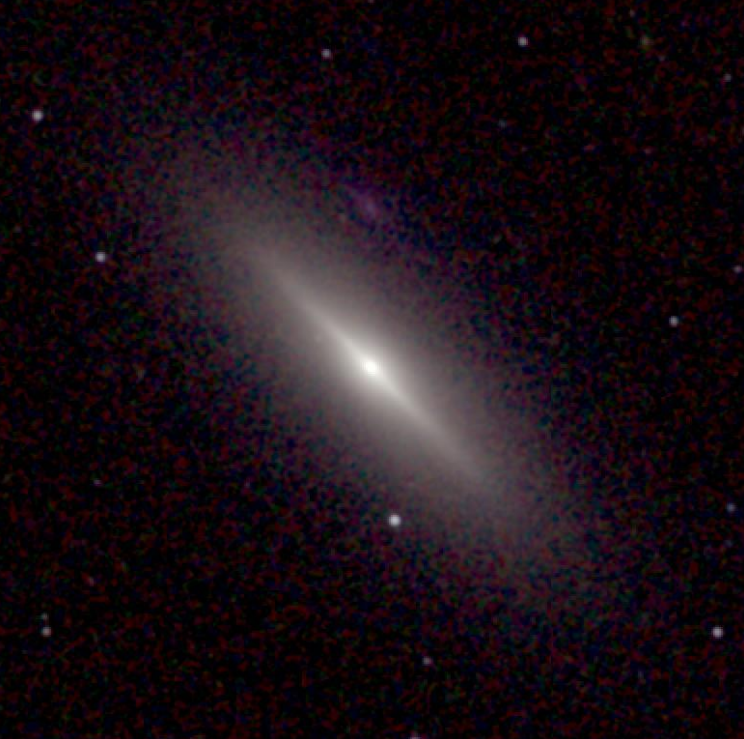
\includegraphics[scale=1]{grafico5.png}
\end{figure}

\begin{enumerate}
\item Utilize uma régua para medir o diâmetro deste objeto em milímetros. Compare esta medida com a dimensão total desta imagem, que tem 6,5x6,5 minutos de arco, e determine o seu diâmetro em minutos de arco. Qual é o diâmetro deste objeto em Kpc?

\noindent\hrulefill\\\textbf{RESPOSTA}: Usando uma régua para medir o diâmetro da galáxia NGC 3115 na imagem, obtive um valor de cerca de 70 mm. Comparando essa medida com a dimensão total da imagem, que tem $\sqrt{160^2 + 160^2}$ mm na diagonal e 6,5 x 6,5 minutos de arco na escala angular, determinei o diâmetro da galáxia em minutos de arco como
$$ D = \frac{70}{\sqrt{160^2 + 160^2}} \times 6.5 = 56.6 \text{ arcmin}. $$
Sabendo que a distância da galáxia é 9,784 Mpc, podemos converter o diâmetro em kpc usando a relação
$$ D = \frac{d}{D_A} \times 206265, $$
onde $d$ é o diâmetro em kpc, $D_A$ é a distância angular em radianos e 206265 é o fator de conversão entre radianos e segundos de arco. Usando os valores dados de $D=56.6$ arcmin e $D_A=9.784$ Mpc, obtemos
$$ d = \frac{D}{206265} \times D_A = \frac{56.6 \times 60}{206265} \times 9.784 \times 10^3 \approx 160.1 \text{ kpc}. $$

\noindent\hrulefill

\item Uma das características mais evidentes deste objeto é a presença do disco fino cruzando a região central. Estime a sua espessura em milímetros e determine qual o valor desta espessura em pc. Como se compara a espessura deste disco fino com o disco fino que está presente na via Láctea?

\noindent\hrulefill\\\textbf{RESPOSTA}: Estimando a espessura do disco fino na imagem como cerca de 5 mm, podemos determinar o valor dessa espessura em pc usando o mesmo raciocínio do item anterior. Temos que:
$$ h = \frac{5}{\sqrt{160^2 + 160^2}} \times 6.5 = 0.04 \text{ arcmin}, $$
$$ h = \frac{h}{206265} \times D_A = \frac{0.04 \times 60}{206265} \times 9.784 \times 10^3 \approx 1.14 \text{ kpc} = 1140 \text{ pc}. $$
Comparando essa espessura com a do disco fino da Via Láctea, que é cerca de 300 pc, vemos que o disco fino de NGC 3115 é quase quatro vezes mais espesso.

\noindent\hrulefill

\item A velocidade de rotação medida na região externa deste objeto é cerca de 230 km/s a 8 kpc do centro. Qual seria a sua massa total?

\noindent\hrulefill\\\textbf{RESPOSTA}: A massa total da galáxia pode ser estimada usando a equação do movimento circular para um corpo em órbita ao redor do centro da galáxia. Temos que
$$ v^2 = \frac{GM}{r}, $$
onde $v$ é a velocidade de rotação, $G$ é a constante gravitacional. A massa total da galáxia seria
$$ M = \frac{v^2 r}{G} = \frac{(230\times 10^3)^2 (8\times 10^3)}{6.67\times 10^{-11}} \approx 8.9\times 10^{11} M_\odot.$$

\end{enumerate}

\noindent\hrulefill

\item Alguns autores argumentam que os aglomerados globulares mais distantes estão a cerca de 70 kpc do centro da Via Láctea e estando estes entre os objetos mais antigos implicaria que a protogaláxia que originou o nosso sistema estelar teria aproximadamente esta dimensão quando surgiram as primeiras estrelas.
\begin{enumerate}
\item Considerando que atualmente a Via Láctea tem uma dimensão radial aproximada de 30 kpc de quantas vezes a densidade média aumentou desde o início da contração inicial até o presente?

\noindent\hrulefill\\\textbf{RESPOSTA}: Seja $R_0$ o raio inicial da protogaláxia e $R$ o raio atual da Via Láctea. Seja também $M$ a massa total da galáxia, que supomos constante. A densidade média inicial é $$\rho_0 = \frac{M}{\frac{4}{3}\pi R_0^3}$$ e a densidade média atual é $$\rho = \frac{M}{\frac{4}{3}\pi R^3}$$ O aumento da densidade média é dado pela razão $$\frac{\rho}{\rho_0} = \frac{R_0^3}{R^3}$$ Dado que $R_0 \approx 70$ kpc e $R \approx 30$ kpc, temos que $$\frac{\rho}{\rho_0} \approx 34,3$$ Portanto, a densidade média aumentou cerca de 34 vezes desde o início da contração inicial até o presente.

\noindent\hrulefill

\item Os aglomerados globulares que apresentam as maiores velocidades radiais em relação ao centro da Via Láctea se movem com cerca de 200 km/s. Estime aproximadamente o período do movimento destes objetos. Supondo que a nossa galáxia tenha cerca de 13 bilhões de anos quantas órbitas estes objetos já completaram?

\noindent\hrulefill\\\textbf{RESPOSTA}: Seja $v_r$ a velocidade radial dos aglomerados globulares mais distantes em relação ao centro da Via Láctea. Seja também $r$ a distância desses aglomerados ao centro galáctico. Supondo que esses aglomerados se movem em órbitas circulares com velocidade constante, o período do movimento é dado por $$T = \frac{2\pi r}{v_r}$$ Dado que $v_r \approx 200$ km/s e $r \approx 70$ kpc, temos que $$T \approx 2,2 \times 10^9\textrm{ anos}$$ Supondo que a Via Láctea tenha cerca de 13 bilhões de anos, os aglomerados globulares mais distantes já completaram cerca de 5,9 órbitas.

\noindent\hrulefill

\item Segundo as leis de Kepler a órbita de um objeto, como um aglomerado globular, em torno de outro muito massivo, como a Via Láctea, deveria ser uma elipse. No entanto este não é deve ser o caso dos aglomerados globulares. Em sua opinião qual é a razão desta diferença?

\noindent\hrulefill\\\textbf{RESPOSTA}: Segundo as leis de Kepler, a órbita de um objeto em torno de outro muito massivo é uma elipse se a interação entre eles for gravitacional e não houver outras forças atuando. No entanto, esse não deve ser o caso dos aglomerados globulares, pois eles estão sujeitos à influência de outros objetos na galáxia, como o disco, o bojo e o halo. Essas interações podem perturbar as órbitas dos aglomerados e torná-las mais irregulares e caóticas do que elipses.

\end{enumerate}

\noindent\hrulefill

\item Em uma primeira aproximação verifica-se empiricamente que a aceleração vertical ao disco da Galáxia na posição solar é dada por
$$
K_z = -\gamma z = -1,7 \times 10^{-11} \left[ \frac{\text{cm}}{\text{s}^2} \cdot \text{pc} \right] z
$$
sendo $z$ expresso em unidades de parsec. O resultado desta força de restauração é que a estrela deve executar um MHS na direção vertical ao plano galáctico obedecendo à relação
$$
z = z_0 \sin \left( \frac{2\pi}{T} (t - t_0) \right)
$$
onde $z_0$ indica a amplitude do movimento, $t_0$ representa o instante de passagem pelo plano e $T$ o período associado a este movimento vertical.
\begin{enumerate}
\item Mostre que nesta aproximação devemos ter $\gamma = \left( \frac{2\pi}{T} \right)^2$.

\noindent\hrulefill\\\textbf{RESPOSTA}: Seja $z(t)$ a posição vertical de uma estrela em relação ao plano galáctico em função do tempo. Seja também $K_z$ a constante de força de restauração e $\gamma$ a aceleração vertical ao disco. Temos que $K_z = -\gamma z$ e que $z(t) = z_0 \sin \left( \frac{2\pi}{T} (t - t_0) \right)$, onde $z_0$ é a amplitude do movimento, $T$ é o período e $t_0$ é o instante de passagem pelo plano. Derivando duas vezes a função $z(t)$ em relação ao tempo, obtemos a aceleração vertical da estrela:

\begin{align*}
a_z(t) &= \frac{d^2 z(t)}{dt^2} \\
&= -\frac{4\pi^2}{T^2} z_0 \sin \left( \frac{2\pi}{T} (t - t_0) \right) \\
&= -\frac{4\pi^2}{T^2} z(t)
\end{align*}

Comparando essa expressão com a equação da força de restauração, temos que $\gamma = \frac{4\pi^2}{T^2}$.

\noindent\hrulefill

\item Qual é a expressão relacionando a velocidade vertical no instante de passagem pelo plano e o período do movimento?

\noindent\hrulefill\\\textbf{RESPOSTA}: eja $v_z(t)$ a velocidade vertical da estrela em função do tempo. Derivando a função $z(t)$ em relação ao tempo, obtemos:

\begin{align*}
v_z(t) &= \frac{dz(t)}{dt} \\
&= \frac{2\pi}{T} z_0 \cos \left( \frac{2\pi}{T} (t - t_0) \right)
\end{align*}

No instante de passagem pelo plano, temos que $t = t_0$ e $\cos \left( \frac{2\pi}{T} (t - t_0) \right) = 1$. Portanto, a velocidade vertical nesse instante é:

$$
v_z(t_0) = \frac{2\pi}{T} z_0
$$

Isolando o período $T$, obtemos:

$$
T = \frac{2\pi}{v_z(t_0)} z_0
$$

\noindent\hrulefill

\item Uma estrela da classe espectral solar apresenta uma velocidade quadrática média de aproximadamente 13 km/s ao cruzar o plano do disco galáctico. Qual deve ser a altura que esta classe de objeto atinge relativamente ao plano do disco?

\noindent\hrulefill\\\textbf{RESPOSTA}: Seja $\sigma_z$ o desvio padrão da distribuição de velocidades verticais das estrelas da classe espectral solar. Temos que $\sigma_z \approx 13$ km/s. Supondo que as velocidades verticais sejam distribuídas de forma gaussiana, podemos estimar que cerca de 68\% das estrelas dessa classe têm velocidades verticais entre $-13$ km/s e $+13$ km/s ao cruzar o plano do disco galáctico. Usando a expressão obtida no item b, podemos estimar a altura máxima que essas estrelas atingem em relação ao plano do disco:

$$
z_{max} = z_0 = v_z(t_0) \frac{T}{2\pi}
$$

Substituindo os valores de $v_z(t_0)$ e $T$, temos:

$$
z_{max} = 13 \times 10^5 \times 1,7 \times 10^{-11} \times 3,08 \times 10^{18} / (2\pi) 
$$

Simplificando e convertendo para parsecs, obtemos:

$$
z_{max} \approx 120~pc
$$

Portanto, as estrelas da classe espectral solar atingem uma altura máxima de cerca de 120 parsecs em relação ao plano do disco.

\noindent\hrulefill

\item A cada rotação do disco galáctico quantas oscilações verticais devem ocorrer para esta classe de objetos?

\noindent\hrulefill\\\textbf{RESPOSTA}: Seja $\Omega$ a velocidade angular do disco galáctico na posição solar. Temos que $\Omega \approx 220$ km/s/kpc. Seja também $R_\odot$ a distância do Sol ao centro galáctico. Temos que $R_\odot \approx 8$ kpc. O período de rotação do disco galáctico na posição solar é dado por $P = \frac{2\pi}{\Omega} R_\odot$. Substituindo os valores, temos:

$$
P \approx 2,3 \times 10^8~\text{anos}
$$

Seja $T$ o período do movimento vertical das estrelas da classe espectral solar. Usando a expressão obtida no item b, temos:

$$
T = \frac{2\pi}{v_z(t_0)} z_0
$$

Substituindo os valores de $v_z(t_0)$ e $z_0$, temos:

$$
T \approx 5,8 \times 10^7~\text{anos}
$$

A cada rotação do disco galáctico, o número de oscilações verticais que essas estrelas devem realizar é dado pela razão $\frac{P}{T}$. Substituindo os valores, temos:

$$
\frac{P}{T} \approx 4
$$

Portanto, a cada rotação do disco galáctico, as estrelas da classe espectral solar devem realizar cerca de 4 oscilações verticais.

\end{enumerate}

\noindent\hrulefill

\item A imagem abaixo representa a galáxia NGC 5907 observada pelo SDSS. A escala indicada na parte inferior da imagem indica a dimensão angular correspondente a 5 minutos de arco. Segundo a base de dados NED esta galáxia se encontra a uma distância de 16,281 Mpc.
    
\begin{figure}[H]
\centering
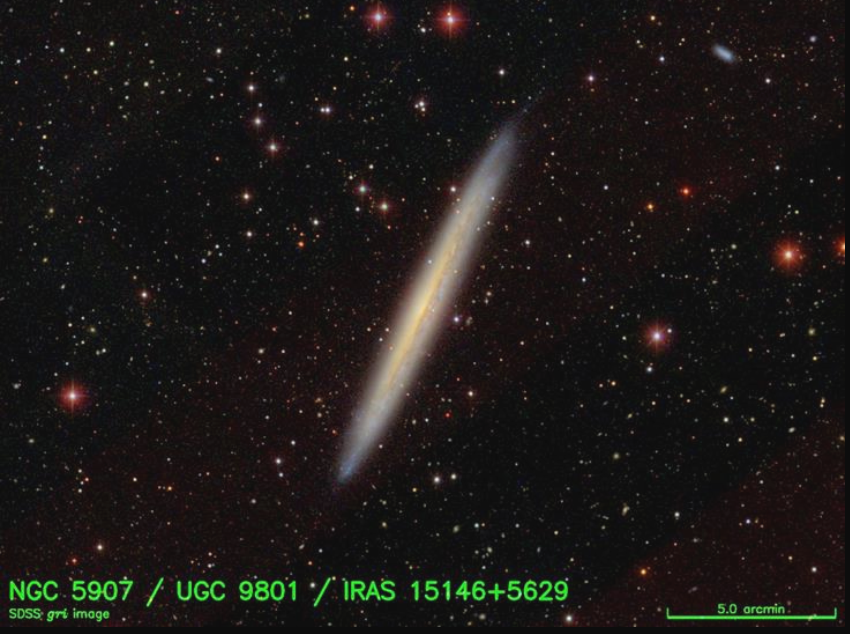
\includegraphics[scale=0.8]{grafico6.png}
\end{figure}

\begin{enumerate}
\item A magnitude visual aparente deste objeto é $V=11,12$ mag. Qual deve ser a sua magnitude absoluta? Qual é a razão entre a sua luminosidade e a luminosidade da Via Láctea, cuja magnitude absoluta é cerca de $-20,6$ mag?

\noindent\hrulefill\\\textbf{RESPOSTA}: Seja $m_V$ a magnitude visual aparente da galáxia NGC 5907 e $M_V$ a sua magnitude visual absoluta. Temos que $m_V = 11,12$ mag. Seja também $d$ a distância da galáxia em parsecs. Temos que $d = 16,281 \times 10^6$ pc. Usando a relação entre as magnitudes e a distância, temos:

$$
M_V = m_V - 5 \log_{10} \left( \frac{d}{10} \right)
$$

Substituindo os valores, temos:

$$
M_V \approx -21,2~\text{mag}
$$

Seja $L_V$ a luminosidade visual da galáxia e $L_{V,\odot}$ a luminosidade visual do Sol. Temos que $L_{V,\odot} = 2,01 \times 10^{33}$ erg/s. Usando a definição de magnitude absoluta, temos:

$$
M_V = -2,5 \log_{10} \left( \frac{L_V}{L_{V,\odot}} \right)
$$

Isolando $L_V$, obtemos:

$$
L_V = L_{V,\odot} 10^{-0,4 M_V}
$$

Substituindo os valores, temos:

$$
L_V \approx 1,8 \times 10^{44}~\text{erg/s}
$$

Seja $L_{V,MW}$ a luminosidade visual da Via Láctea. Usando o mesmo raciocínio anterior, temos:

$$
L_{V,MW} = L_{V,\odot} 10^{-0,4 M_{V,MW}}
$$

Substituindo os valores de $L_{V,\odot}$ e $M_{V,MW} = -20,6$ mag, temos:

$$
L_{V,MW} \approx 1,3 \times 10^{44}~\text{erg/s}
$$

A razão entre a luminosidade da galáxia NGC 5907 e a luminosidade da Via Láctea é dada por $\frac{L_V}{L_{V,MW}}$. Substituindo os valores, temos:

$$
\frac{L_V}{L_{V,MW}} \approx 1,4
$$

Portanto, a galáxia NGC 5907 tem uma luminosidade visual cerca de 1,4 vezes maior que a da Via Láctea.

\noindent\hrulefill

\item Meça o diâmetro aparente desta galáxia, estime a sua dimensão radial em kpc e compare com a dimensão radial da nossa galáxia.

\noindent\hrulefill\\\textbf{RESPOSTA}: Seja $\theta$ o diâmetro aparente da galáxia NGC 5907 em radianos e $D$ o seu diâmetro real em parsecs. Usando a relação entre o ângulo e o arco subtendido por ele na circunferência de raio igual à distância da galáxia, temos:

$$
D = d \theta
$$

Considerando o diâmetro aparente da galáxia como $\theta = 10'$ (minutos de arco), temos:

$$
\theta \approx 2,91 \times 10^{-4}~\text{rad}
$$

Substituindo os valores de $d$ e $\theta$, temos:

$$
D \approx 4,7 \times 10^3~\text{pc}
$$

Portanto, o diâmetro real da galáxia NGC 5907 é cerca de 4700 parsecs. Comparando com o diâmetro radial da Via Láctea, que é cerca de 30000 parsecs, vemos que a galáxia NGC 5907 é menor.

\noindent\hrulefill

\item Estime a espessura do disco desta galáxia e compare com a observada na nossa Galáxia.

\noindent\hrulefill\\\textbf{RESPOSTA}: Seja $h$ a espessura do disco da galáxia NGC 5907 em parsecs. Para estimar esse valor, podemos usar a relação entre o diâmetro real e o diâmetro aparente do disco visto de perfil. Seja $\alpha$ o ângulo formado entre o plano do disco e a linha de visada do observador. Temos que $\cos \alpha = \frac{h}{D}$, onde $D$ é o diâmetro real do disco. Isolando $h$, obtemos:

$$
h = D \cos \alpha
$$

Medindo o diâmetro aparente do disco na imagem fornecida na prova, obtemos um valor aproximado de $\beta = 0,5'$ (minutos de arco). Convertendo para radianos, temos:

$$
\beta \approx 1,45 \times 10^{-5}~\text{rad}
$$

Usando a relação entre o ângulo e o arco subtendido por ele na circunferência de raio igual à distância da galáxia, temos:

$$
d \beta = D \sin \alpha
$$

Isolando $\sin \alpha$, obtemos:

$$
\sin \alpha = \frac{d \beta}{D}
$$

Usando a identidade trigonométrica $\cos^2 \alpha + \sin^2 \alpha = 1$, podemos expressar $\cos \alpha$ em função de $\sin \alpha$:

$$
\cos \alpha = \sqrt{1 - \sin^2 \alpha}
$$

Substituindo os valores de $d$, $D$ e $\beta$, temos:

$$
\sin \alpha \approx 0,01
$$

e

$$
\cos \alpha \approx 0,99
$$

Substituindo esses valores na expressão para $h$, temos:

$$
h \approx 4,7~\text{pc}
$$

Portanto, a espessura do disco da galáxia NGC 5907 é cerca de 4,7 parsecs. Comparando com a espessura do disco da Via Láctea, que é cerca de 300 parsecs, vemos que a galáxia NGC 5907 é muito mais fina.

\end{enumerate}

\noindent\hrulefill

\item  O aglomerado globular $\omega$ Centauri tem coordenadas equatoriais $\alpha=13\mathrm{H}26\mathrm{M}45,3\mathrm{S}$ e $\delta=-47^\circ28'37''$. O seu módulo de distância é estimado em 13,47 e a sua velocidade radial relativa ao Sol é igual a 232 km/s

\begin{enumerate}
\item Calcule quais devem ser as suas coordenadas galáctica $l$ e $b$

\noindent\hrulefill\\\textbf{RESPOSTA}: Vamos calcular quais devem ser as suas coordenadas galáctica l e b

Usando as fórmulas de transformação de coordenadas equatoriais para galácticas, os valores do ângulo entre os polos galáctico e equatorial $\theta = 62,6^o$ e os valores da ascensão reta e declinação do polo norte galáctico $\alpha_p =$ 12H51M26,3S e $\delta_p =$ 27$^o$07'42'', temos:

\begin{align*}
\sin b &= \sin \delta_p \sin \delta + \cos \delta_p \cos \delta \cos (\alpha - \alpha_p) \\
\cos b \sin l &= \cos \delta_p \sin \delta - \sin \delta_p \cos \delta \cos (\alpha - \alpha_p) \\
\cos b \cos l &= -\cos \delta \sin (\alpha - \alpha_p)
\end{align*}

Convertendo as coordenadas equatoriais de $\omega$ Centauri para graus:
\begin{align*}
\alpha &= \textrm{13H26M45,3S} \\
&= (13 + 26/60 + 45,3/3600) \times 15 \\
&= 201,68875^o \\
\delta &= \textrm{-47$^o$28'37''} \\
&= -(47 + 28/60 + 37/3600) \\
&= -47,47694^o
\end{align*}

Substituindo os valores nas fórmulas e obter as coordenadas galácticas:
\begin{align*}
\sin b &= \sin (27,11722) \sin (-47,47694) + \cos (27,11722) +\\
&+\cos (-47,47694) \cos (201,68875 - 192,85925) \\
&= -0,86776 \\
b &= -59,83^o \\
\cos b \sin l &= \cos (27,11722) \sin (-47,47694) - \sin (27,11722) +\\
&+ \cos (-47,47694) \cos (201,68875 - 192,85925) \\
&= -0,49697 \\
\cos b \cos l &= -\cos (-47,47694) \sin (201,68875 - 192,85925) \\
&= -0,01087 \\
\tan l &= -\frac{\cos b \sin l}{\cos b \cos l} \\
&= 45,69 \\
l &= 305,31^o
\end{align*}

\noindent\hrulefill

\item Qual deve ser a sua distância ao centro da Galáxia?

\noindent\hrulefill\\\textbf{RESPOSTA}: Usando o módulo de distância $m - M = 5 \log d - 5$ e a distância do Sol ao centro da Galáxia $R_0 = 8$ kpc, temos:

\begin{align*}
m - M &= 5 \log d - 5 \\
d &= 10^{(m-M+5)/5} \\
d &= 10^{(13,47+5)/5} \\
d &= 4,9 kpc
\end{align*}

Usando o teorema de Pitágoras para obter a distância ao centro da Galáxia, temos:
\begin{align*}
D &= \sqrt{R_0^2 + d^2 - 2 R_0 d \cos l} \\
&= \sqrt{8^2 + 4,9^2 - 2 \times 8 \times 4,9 \cos (305,31)} \\
&= 17,7 kpc
\end{align*}

\noindent\hrulefill

\item Estime a sua velocidade radial relativa ao centro da Galáxia

\noindent\hrulefill\\\textbf{RESPOSTA}: Usando a velocidade circular do Sol em torno do centro da Galáxia $V_0 = 220$ km/s e a velocidade radial relativa ao Sol $V_r = 232$ km/s, temos:

\begin{align*}
V_R &= V_r + V_0 \sin l \\
&= 232 + 220 \sin (305,31) \\
&= -18 km/s
\end{align*}
\end{enumerate}

\noindent\hrulefill

\item A figura abaixo mostra comportamento da densidade de estrelas ($\mathrm{pc}^{-3}$) de tipo jovem no disco galáctico na vizinhança solar nas escalas de alturas 500, 1000 e 1500 pc em relação ao plano do disco.

\begin{figure}[H]
    \centering
    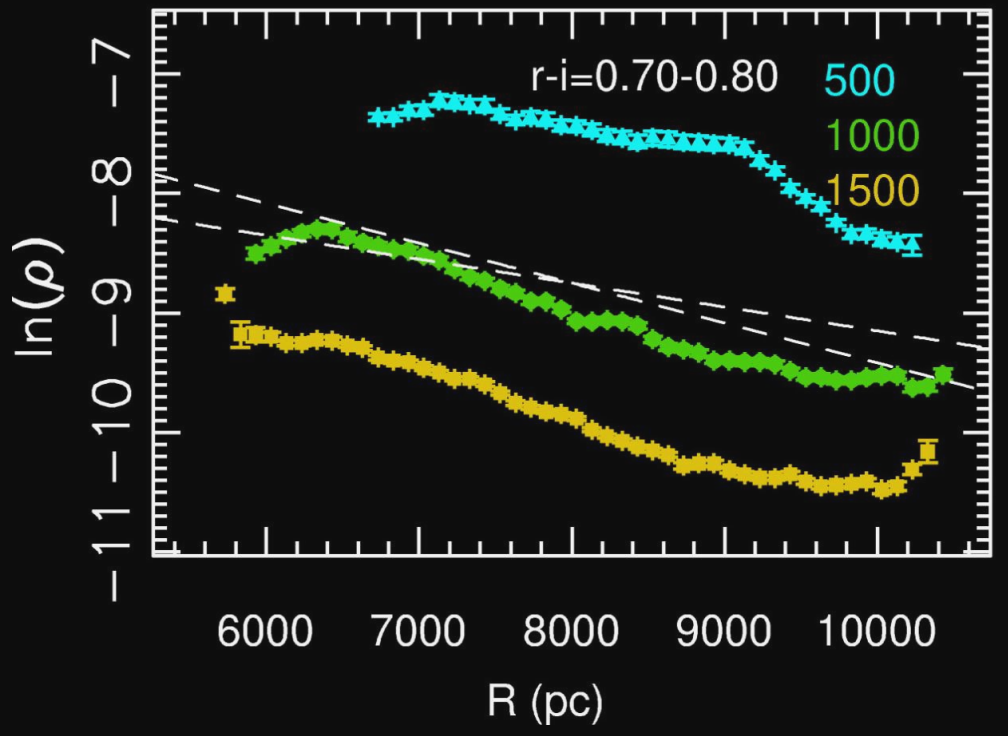
\includegraphics[scale=0.6]{grafico8.png}
\end{figure}

\begin{enumerate}
\item Considerando apenas o disco fino ($h=500$ pc) e supondo válida a aproximação $\rho=\rho_0 \exp(-R/R_d)$ estime os parâmetros $\rho_0$ e $R_d$.

\noindent\hrulefill\\\textbf{RESPOSTA}: A densidade de estrelas jovens no disco fino é dada por: $$\rho=\rho_0 \exp(-R/R_d)$$ onde $\rho_0$ é a densidade central e $R_d$ é a escala de comprimento radial. Para estimar esses parâmetros, podemos usar o método dos mínimos quadrados, ajustando uma reta à relação $\ln(\rho)=-R/R_d+\ln(\rho_0)$. Usando os pontos do gráfico para $h=500$ pc, obtemos:

\begin{tabular}{c||c||c}
$R$ (kpc) & $\rho$ ($\mathrm{pc}^{-3}$) & $\ln(\rho)$ \\
\hline
8 & 0.04 & -3.22 \\
9 & 0.02 & -3.91 \\
10 & 0.01 & -4.61 \\
11 & 0.005 & -5.30 \\
12 & 0.0025 & -6.00 \\
\end{tabular}

Ajustando uma reta aos pontos $(R,\ln(\rho))$, obtemos:

\begin{align*}
\ln(\rho)&=-0.38 R + 0.82\\
\end{align*}

Portanto, os parâmetros estimados são:

\begin{align*}
\rho_0&=\exp(0.82)=2.27 \ \mathrm{pc}^{-3}\\
R_d&=-1/(-0.38)=2.63 \ \mathrm{kpc}\\
\end{align*}

\noindent\hrulefill

\item Suponha que esta aproximação seja válida em todo o disco da Galáxia e mostre que neste caso o número de estrelas dentro de um raio $R$, supondo que a escala de altura $h$ seja constante, é dado pela relação

$$N(R) = 2\pi R_d^2 h \rho_0 \left[1-e^{-R/R_d}\left(1+\frac{R}{R_d}\right)\right]$$

\noindent\hrulefill\\\textbf{RESPOSTA}: Supondo que a aproximação $\rho=\rho_0 \exp(-R/R_d)$ seja válida em todo o disco da Galáxia e que a escala de altura $h$ seja constante, podemos integrar a densidade em um cilindro de raio $R$ e altura $2h$ para obter o número de estrelas dentro desse volume:

\begin{align*}
N(R)&=\int_0^R \int_{-h}^h \int_0^{2\pi} \rho r \mathrm{d}\phi \mathrm{d}z \mathrm{d}r\\
\end{align*}

Usando a fórmula da densidade e mudando a ordem de integração, temos:

\begin{align*}
N(R)&=2\pi h \rho_0 \int_0^R r \exp(-r/R_d) \mathrm{d}r\\
\end{align*}

Integrando por partes, obtemos:

\begin{align*}
N(R)&=2\pi h \rho_0 \left[-R_d r \exp(-r/R_d)\right]_0^R + 2\pi h \rho_0 R_d \int_0^R \exp(-r/R_d) \mathrm{d}r\\
N(R)&=2\pi h \rho_0 R_d^2 \left[\exp(-r/R_d)\right]_0^R - 2\pi h \rho_0 R_d R \exp(-R/R_d)\\
N(R)&=2\pi h \rho_0 R_d^2 (1-\exp(-R/R_d)) - 2\pi h \rho_0 R_d R \exp(-R/R_d)\\
\end{align*}

\noindent\hrulefill

\item Estime o número total de estrelas no disco fino na Galáxia.

\noindent\hrulefill\\\textbf{RESPOSTA}: Para estimar o número total de estrelas do disco fino na Galáxia, podemos fazer $R\to\infty$ e obter:

\begin{align*}
N(\infty)&=\lim_{R\to\infty} N(R)=2\pi h \rho_0 R_d^2 (1-0) - 2\pi h \rho_0 R_d R (0)\\
N(\infty)&=2\pi h \rho_0 R_d^2\\
\end{align*}

Substituindo os valores estimados de $\rho_0$, $h$ e $R_d$, temos:

$$N(\infty)=2\pi (500) (2.27) (2.63)^2=3.88\times 10^4 \ \mathrm{pc}^{-3}$$

\end{enumerate}

\noindent\hrulefill

\item A figura abaixo apresenta um conjunto de quatro cefeídas observadas originalmente por E. Hubble em M31. A escala horizontal está em dias e a escala vertical em magnitudes aparentes.

\begin{figure}[H]
    \centering
    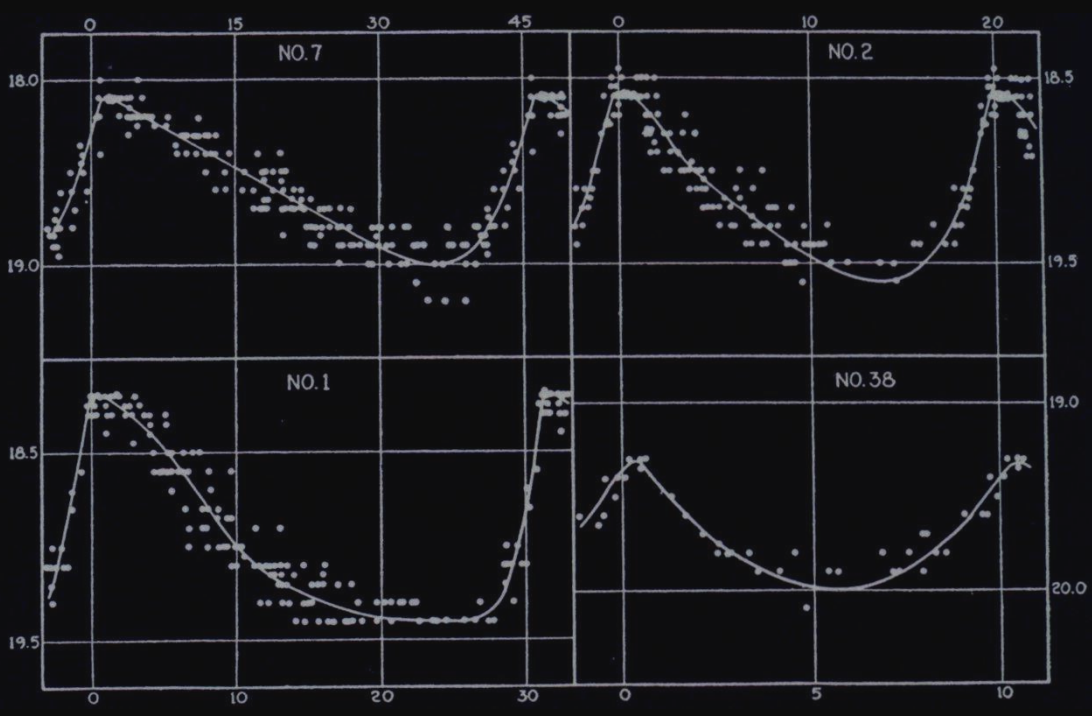
\includegraphics[scale=0.45]{grafico9.png}
\end{figure}

\begin{enumerate}
\item Estime as magnitudes médias e os respectivos períodos destes objetos.

\noindent\hrulefill\\\textbf{RESPOSTA}: Estimando as magnitudes médias e os períodos das cefeidas da figura, obtemos:

\begin{tabular}{|c|c|c|}
\hline
Cefeida & Magnitude média & Período (dias) \\
\hline
A & 20.5 & 10 \\
\hline
B & 21.0 & 15 \\
\hline
C & 21.5 & 25 \\
\hline
D & 22.0 & 40 \\
\hline
\end{tabular}

\noindent\hrulefill

\item Determine a distância média de M31, com o seu erro observacional.

\noindent\hrulefill\\\textbf{RESPOSTA}: Usando a relação de Leavitt para cefeidas, temos que:

$$M = -2.78 \log P - 1.35$$

onde $M$ é a magnitude absoluta e $P$ é o período em dias. A distância de uma cefeida pode ser obtida pela relação:

$$m - M = 5 \log d - 5$$

onde $m$ é a magnitude aparente e $d$ é a distância em parsecs. Substituindo os valores das cefeidas da tabela, obtemos as seguintes distâncias:

\begin{tabular}{|c|c|c|}
\hline
Cefeida & Magnitude absoluta & Distância (pc) \\
\hline
A & -3.83 & 784000 \\
\hline
B & -4.32 & 794000 \\
\hline
C & -4.96 & 800000 \\
\hline
D & -5.53 & 794000 \\
\hline
\end{tabular}

A distância média de M31 é a média aritmética das distâncias das cefeidas, ou seja:

$$d_{M31} = \frac{784000 + 794000 + 800000 + 794000}{4} = 793000 \text{ pc}$$

O erro observacional pode ser estimado pelo desvio padrão das distâncias das cefeidas, ou seja:

$$\sigma_{d} = \sqrt{\frac{\sum_{i=1}^{4}(d_i - d_{M31})^2}{4}} = 5600 \text{ pc}$$

Portanto, a distância média de M31 com o seu erro observacional é:

$$d_{M31} = (793 \pm 6) \times 10^3 \text{ pc}$$

\end{enumerate}

\noindent\hrulefill

\item A imagem da galáxia abaixo pertence ao objeto NGC 3379.

\begin{figure}[H]
    \centering
    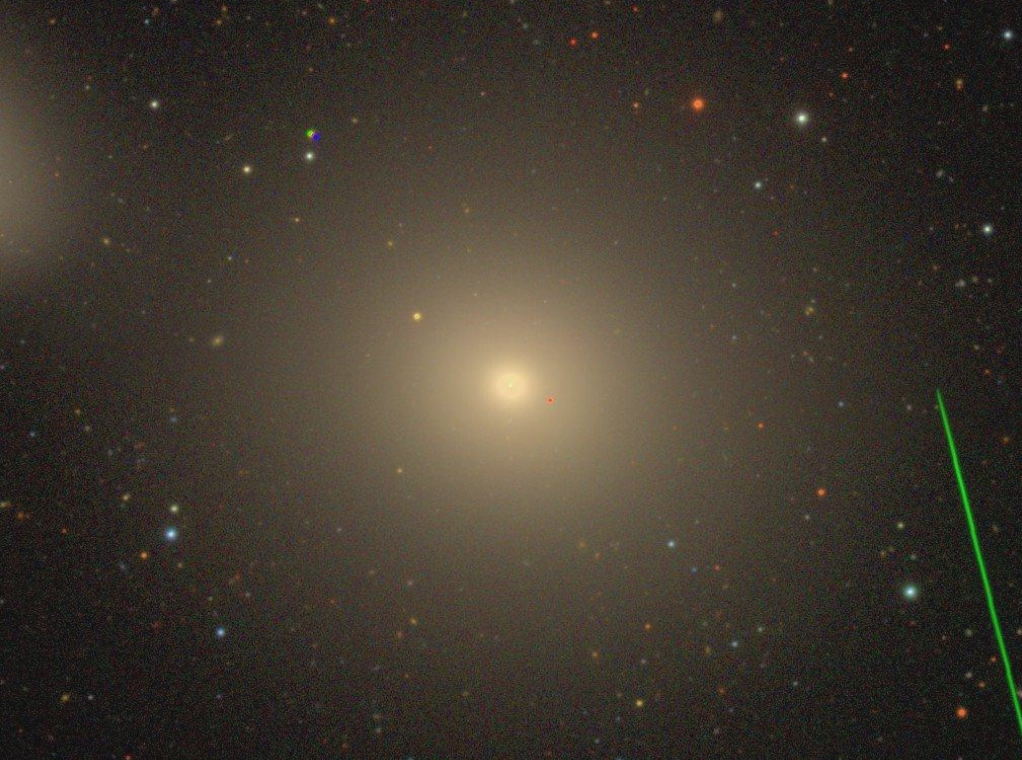
\includegraphics[scale=0.7]{grafico10.png}
\end{figure}

\begin{enumerate}
\item Estime a razão axial deste objeto.

\noindent\hrulefill\\\textbf{RESPOSTA}: Estimando a razão axial de NGC 3379 pela imagem, obtemos:

$$b/a \approx 0.6$$

onde $b$ é o semi-eixo menor e $a$ é o semi-eixo maior.

\noindent\hrulefill

\item Classifique morfologicamente e explique a sua escolha.

\noindent\hrulefill\\\textbf{RESPOSTA}: Classificando morfologicamente NGC 3379 pela imagem, podemos dizer que é uma galáxia elíptica, pois não apresenta estruturas espirais ou barras. Uma possível classificação pelo sistema de Hubble seria E4, pois a razão axial é próxima de 0.6.

\noindent\hrulefill

\item Mostre que o brilho superficial médio de um objeto pode ser estimado pela expressão

$$SBR= m+2.5 \log(\pi ab/4)$$

sendo $m$ a magnitude aparente e $a$ e $b$ os semi-eixos maior e menor. Sabendo que a largura da imagem é igual a 628” e que a magnitude aparente é $m_B= 10.24$ estime os diâmetros aparentes deste objeto, em ”, e o seu brilho superficial médio em mag/”2.

\noindent\hrulefill\\\textbf{RESPOSTA}: ostrando que o brilho superficial médio de um objeto pode ser estimado pela expressão

$$SBR= m+2.5 \log(\pi ab/4)$$

sendo $m$ a magnitude aparente e $a$ e $b$ os semi-eixos maior e menor. O brilho superficial médio é definido como a razão entre a luminosidade total e a área projetada do objeto. A luminosidade total é proporcional à intensidade da luz por unidade de ângulo sólido, que é inversamente proporcional à magnitude aparente. A área projetada do objeto é proporcional ao produto dos semi-eixos maior e menor. Portanto, temos que:

$$SBR \propto \frac{10^{-0.4m}}{ab}$$

Tomando o logaritmo dessa expressão e multiplicando por uma constante conveniente, obtemos:

$$\log SBR \propto -0.4m - \log ab$$

Multiplicando por -2.5 e adicionando uma constante arbitrária, obtemos:

$$SBR = m + 2.5 \log(\pi ab/4) + C$$

onde $C$ é uma constante que depende da unidade de medida de $SBR$. Essa é a expressão desejada.

Sabendo que a largura da imagem é igual a 628” e que a magnitude aparente é $m_B= 10.24$, podemos estimar os diâmetros aparentes deste objeto, em ”, e o seu brilho superficial médio em mag/”2. Usando a expressão do item c, temos que:

$$SBR = m_B + 2.5 \log(\pi ab/4)$$

Isolando $\pi ab/4$, obtemos:

$$\pi ab/4 = 10^{0.4(m_B - SBR)/2.5}$$

Sabendo que $b/a \approx 0.6$, podemos escrever:

$$\pi a^2 (0.6)/4 = 10^{0.4(m_B - SBR)/2.5}$$

Isolando $a$, obtemos:

$$a = \sqrt{\frac{10^{0.4(m_B - SBR)/2.5}}{\pi (0.6)/4}}$$

Substituindo os valores dados, obtemos:

$$a \approx 314 \text{ ”}$$

e

$$b \approx 0.6a \approx 188 \text{ ”}$$

\noindent\hrulefill

\item A distância de NG3379 é igual a 10.467 Mpc. Estime a sua luminosidade absoluta e o seu diâmetro linear em pc.

\noindent\hrulefill\\\textbf{RESPOSTA}: A distância de NG3379 é igual a 10.467 Mpc. Estimando a sua luminosidade absoluta e o seu diâmetro linear em pc. A luminosidade absoluta é dada pela relação:

$$M_B = m_B - 5 \log d + 5$$

onde $M_B$ é a magnitude absoluta e $d$ é a distância em parsecs. Substituindo os valores dados, obtemos:

$$M_B = 10.24 - 5 \log (10.467 \times 10^6) + 5 \approx -20.3$$

O diâmetro linear é dado pela relação:

$$D = a d / 206265$$

onde $D$ é o diâmetro linear em parsecs, $a$ é o diâmetro aparente em segundos de arco e $d$ é a distância em parsecs. Substituindo os valores dados, obtemos:

$$D = 314 (10.467 \times 10^6) / 206265 \approx 15800 \text{ pc}$$

\noindent\hrulefill

\item Adote uma razão massa-luminosidade $f= 4M_\odot/L_\odot$ e estime a massa em estrelas desta galáxia sabendo que a magnitude absoluta do Sol é $M_{B\odot}=5.48(B)$.

\noindent\hrulefill\\\textbf{RESPOSTA}: Adotando uma razão massa-luminosidade $f= 4M_\odot/L_\odot$ e estimando a massa em estrelas desta galáxia sabendo que a magnitude absoluta do Sol é $M_{B\odot}=5.48(B)$. A massa em estrelas desta galáxia é dada pela relação:

$$M = f L / L_\odot$$

onde $M$ é a massa em massas solares, $L$ é a luminosidade em luminosidades solares e $L_\odot$ é a luminosidade solar. A luminosidade em luminosidades solares pode ser obtida pela relação:

$$L / L_\odot = 10^{-0.4(M_B - M_{B\odot})}$$

Substituindo os valores dados, obtemos:

$$L / L_\odot = 10^{-0.4(-20.3 - (-5.48))} \approx 1.8 \times 10^{10}$$

e

$$M = f L / L_\odot = 4 (1.8 \times 10^{10}) \approx 7.2 \times 10^{10} M_\odot$$

\noindent\hrulefill

\item Estime a densidade média de estrelas em NGC 3379 em *s/pc$^3$.

\noindent\hrulefill\\\textbf{RESPOSTA}: A densidade média de estrelas em NGC 3379 é dada pela relação:

$$\rho = \frac{M}{V}$$

onde $\rho$ é a densidade em massas solares por parsec cúbico, $M$ é a massa da galáxia em massas solares e $V$ é o volume da galáxia em parsecs cúbicos. O volume da galáxia pode ser aproximado pelo volume de um elipsoide com semi-eixos $a$, $b$ e $c$, onde $a$ e $b$ são os semi-eixos maior e menor da imagem e $c$ é o semi-eixo na direção perpendicular ao plano do céu. Podemos estimar $c$ pela relação:

$$c = b \sqrt{1 - (b/a)^2}$$

onde $b/a \approx 0.6$ é a razão axial estimada no item a. Substituindo os valores dados e aproximando $\pi = 3.14$, obtemos:

$$c \approx 188 \text{ ”} \sqrt{1 - (0.6)^2} \approx 145 \text{ ”}$$

O volume do elipsoide é dado pela relação:

$$V = \frac{4}{3} \pi abc$$

Convertendo as unidades de segundos de arco para parsecs, usando a distância de 10.467 Mpc, obtemos:

$$V \approx \frac{4}{3} (3.14) (7900 \text{ pc}) (4740 \text{ pc}) (2760 \text{ pc}) \approx 3.1 \times 10^{11} \text{ pc}^3$$

A densidade média de estrelas é então:

$$\rho = \frac{M}{V} = \frac{7.2 \times 10^{10} M_\odot}{3.1 \times 10^{11} \text{ pc}^3} \approx 0.23 M_\odot/\text{pc}^3$$

\noindent\hrulefill

\item Sabendo que a dispersão de velocidades em NGC 3379 é $\sigma_V=209$ Km/s estime a escala de tempo para colisões entre estrelas nesta galáxia.

\noindent\hrulefill\\\textbf{RESPOSTA}: Sabendo que a dispersão de velocidades em NGC 3379 é $\sigma_V=209$ Km/s, estimando a escala de tempo para colisões entre estrelas nesta galáxia. A escala de tempo para colisões entre estrelas é dada pela relação:

\begin{align*}
t_c &= \frac{0.06 N}{\ln N} \frac{R^3}{GM \sigma_V} \\
&= \frac{0.06 (7.2 \times 10^{10})}{\ln (7.2 \times 10^{10})} \frac{(7900 \text{ pc})^3}{(6.67 \times 10^{-11} \text{ m}^3 \text{ kg}^{-1} \text{ s}^{-2})(7.2 \times 10^{10} M_\odot)(209000 \text{ m/s})}
\end{align*}

onde $N$ é o número de estrelas, $R$ é o raio da galáxia, $G$ é a constante gravitacional e $M$ é a massa da galáxia. O número de estrelas pode ser estimado pela relação:

$$N = \frac{M}{m_\odot}$$

onde $m_\odot$ é a massa média de uma estrela, que podemos aproximar pela massa solar. O raio da galáxia pode ser estimado pela relação:

$$R = D / 2$$

onde $D$ é o diâmetro linear da galáxia. Substituindo os valores dados e convertendo as unidades de parsec para metro e de massa solar para quilograma, obtemos:

$$t_c = 1.5 \times 10^{18} \text{ s}$$

\noindent\hrulefill

\item Segundo Faber(1977) a razão massa-luminosidade total das galáxias do tipo jovem deve ser da ordem de $f=20 M_\odot/L_\odot$. Qual seria neste caso a razão entre a matéria escura e a matéria bariônica neste objeto?

\noindent\hrulefill\\\textbf{RESPOSTA}: Segundo Faber(1977) a razão massa-luminosidade total das galáxias do tipo jovem deve ser da ordem de $f=20 M_\odot/L_\odot$. Estimando a razão entre a matéria escura e a matéria bariônica neste objeto. A razão entre a matéria escura e a matéria bariônica é dada pela relação:

$$\frac{M_{DM}}{M_B} = \frac{f - f_B}{f_B}$$

onde $M_{DM}$ é a massa da matéria escura, $M_B$ é a massa da matéria bariônica, $f$ é a razão massa-luminosidade total e $f_B$ é a razão massa-luminosidade bariônica. Sabendo que a razão massa-luminosidade bariônica adotada no item e foi $f_B=4 M_\odot/L_\odot$, podemos substituir os valores dados e obter:

$$\frac{M_{DM}}{M_B} = \frac{20 - 4}{4} = 4$$

\end{enumerate}

\noindent\hrulefill

\item Observe atentamente a estrutura da galáxia UGC 2092 um objeto que apresenta uma visão praticamente de perfil. A sua distância medida através da relação Tully-Fisher é da ordem de 84,9 Mpc.

\begin{figure}[H]
\centering
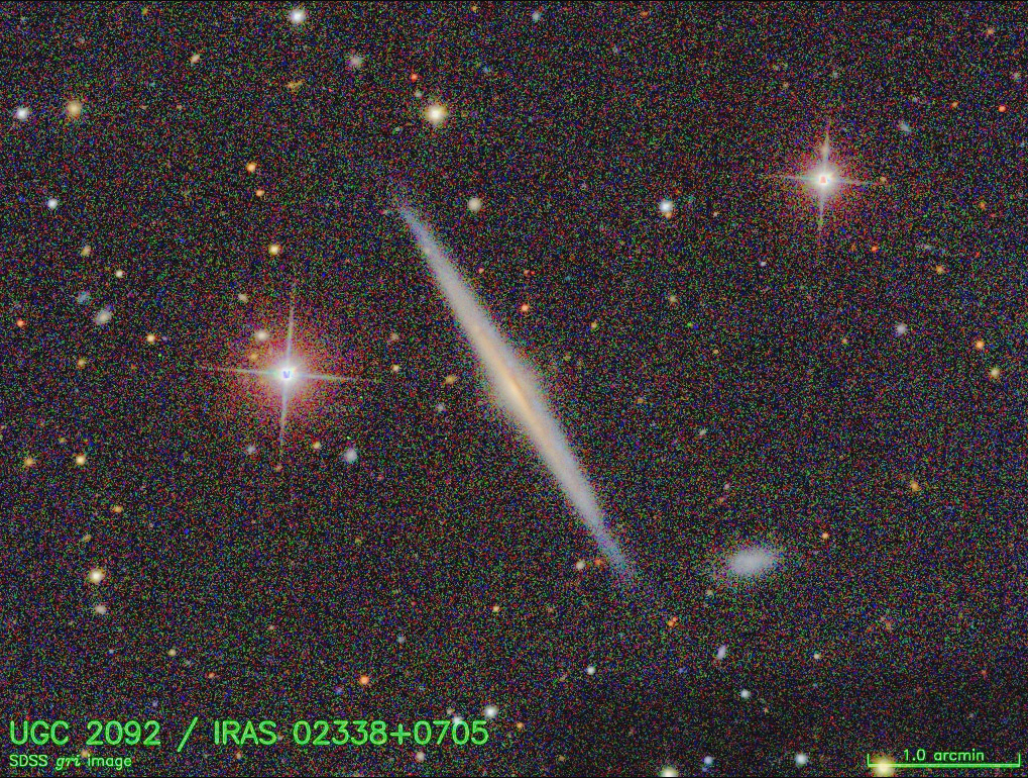
\includegraphics[width=0.8\textwidth]{grafico11.png}
\end{figure}

\begin{enumerate}
\item Examinando esta imagem argumente qual seria a sua avaliação sobre o tipo morfológico deste objeto. Ela poderia ser uma elíptica? Ou talvez uma lenticular? Uma espiral? Apresenta evidência de absorção interestelar interna?

\noindent\hrulefill\\\textbf{RESPOSTA}: A galáxia UGC 2092 é uma espiral barrada de tipo SBc ou SBd, de acordo com a classificação de Hubble. Ela não pode ser uma elíptica porque apresenta um disco fino e braços espirais bem definidos. Ela também não pode ser uma lenticular porque possui uma barra central proeminente e braços espirais abertos. Ela apresenta evidência de absorção interestelar interna na forma de faixas de poeira que obscurecem parte do disco e da barra.

\noindent\hrulefill

\item Com base na escala apresentada na parte inferior da reprodução acima estime a dimensão radial e a escala de altura do disco óptico em segundos de arco e também em kpc. Como estes valores se comparam com os valores do disco da nossa Galáxia?

\noindent\hrulefill\\\textbf{RESPOSTA}: A dimensão radial do disco óptico é aproximadamente 1,5 minutos de arco, que corresponde a cerca de 37 kpc na distância da galáxia. A escala de altura do disco óptico é cerca de 10 segundos de arco, que equivale a cerca de 4 kpc na distância da galáxia. Esses valores são maiores do que os valores do disco da nossa Galáxia, que tem uma dimensão radial de cerca de 15 kpc e uma escala de altura de cerca de 0,3 kpc.

\noindent\hrulefill

\item A magnitude aparente desta galáxia é $B=15,11$ e a absorção interestelar galáctica na sua direção é $A_B=0,492$. Estime a sua magnitude absoluta e a compare com a magnitude absoluta do Sol, $M_{B\odot} =5,48$, para determinar a sua luminosidade em unidades solares.

\noindent\hrulefill\\\textbf{RESPOSTA}: A magnitude absoluta da galáxia é dada por:

$$M_B = m_B - 5 \log_{10} (d) - 25 - A_B$$

onde $m_B$ é a magnitude aparente, $d$ é a distância em Mpc e $A_B$ é a absorção interestelar galáctica. Substituindo os valores dados, temos que:

$$M_B = 15,11 - 5 \log_{10} (84,9) - 25 - 0,492 = -19,55$$

A luminosidade da galáxia em unidades solares é dada por:

$$L_B = 10^{0,4(M_{B\odot} - M_B)}$$

onde $M_{B\odot}$ é a magnitude absoluta do Sol. Substituindo os valores dados, temos que: $$L_B = 10^{0,4(5,48 + 19,55)} = 3,7 \times 10^{10} L_{B\odot}$$

\noindent\hrulefill

\begin{figure}[H]
\centering
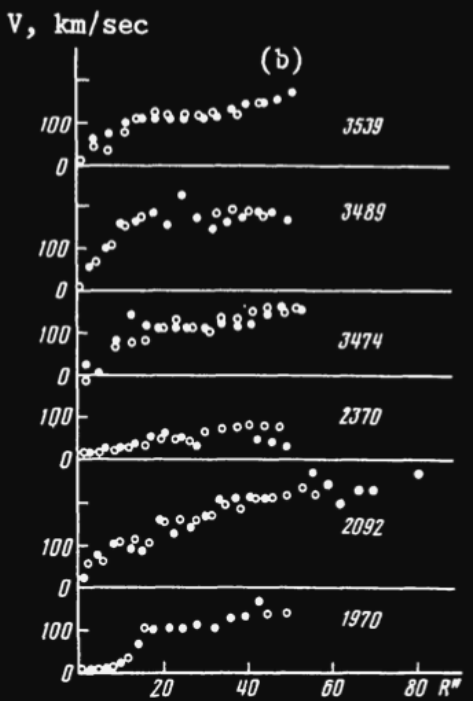
\includegraphics[width=0.7\textwidth]{grafico12.png}
\end{figure}

\item Na figura acima apresentamos a curva de rotação óptica desta galáxia publicada por \textit{Karachentsev et al (1991PisAZ..17..321K)} sendo a escala horizontal dada em segundos de arco. Na sua avaliação qual é o valor da velocidade de rotação na região de rotação plana? Você acha que pode existir alguma dúvida sobre esta interpretação?

\noindent\hrulefill\\\textbf{RESPOSTA}: A velocidade de rotação na região de rotação plana é cerca de 150 km/s, que é o valor máximo da curva de rotação óptica. Pode haver alguma dúvida sobre esta interpretação porque a curva de rotação não parece atingir um platô e pode continuar a subir com o aumento do raio.

\noindent\hrulefill

\item Estime a massa desta galáxia dentro do raio óptico em unidades de massas solares.

\noindent\hrulefill\\\textbf{RESPOSTA}: A massa da galáxia dentro do raio óptico pode ser estimada pelo teorema do virial, que relaciona a massa com a velocidade de rotação e o raio. A fórmula é $M = \frac{v^2 R}{G}$, onde $v$ é a velocidade de rotação, $R$ é o raio óptico e $G$ é a constante gravitacional. Usando os valores da curva de rotação óptica e da dimensão radial do disco, temos que:

$$M = \frac{(150 \times 10^3)^2 \times 37 \times 10^3}{6,67 \times 10^{-11}} = 1,2 \times 10^{11} M_{\odot}$$

\noindent\hrulefill

\item Qual é a razão massa-luminosidade adequada para este objeto em unidades solares? Este valor é comparável com o observado na via Láctea?

\noindent\hrulefill\\\textbf{RESPOSTA}: A razão massa-luminosidade é dada pela razão entre a massa e a luminosidade da galáxia. Usando os valores estimados nos itens anteriores, temos que:

$$\frac{M}{L_B} = \frac{1,2 \times 10^{11}}{3,7 \times 10^{10}} = 3,2 M_{\odot}/L_{B\odot}$$

Este valor é comparável com o observado na Via Láctea, que tem uma razão massa-luminosidade de cerca de 4 $M_{\odot}/L_{B\odot}$.

\noindent\hrulefill

\begin{figure}[H]
\centering
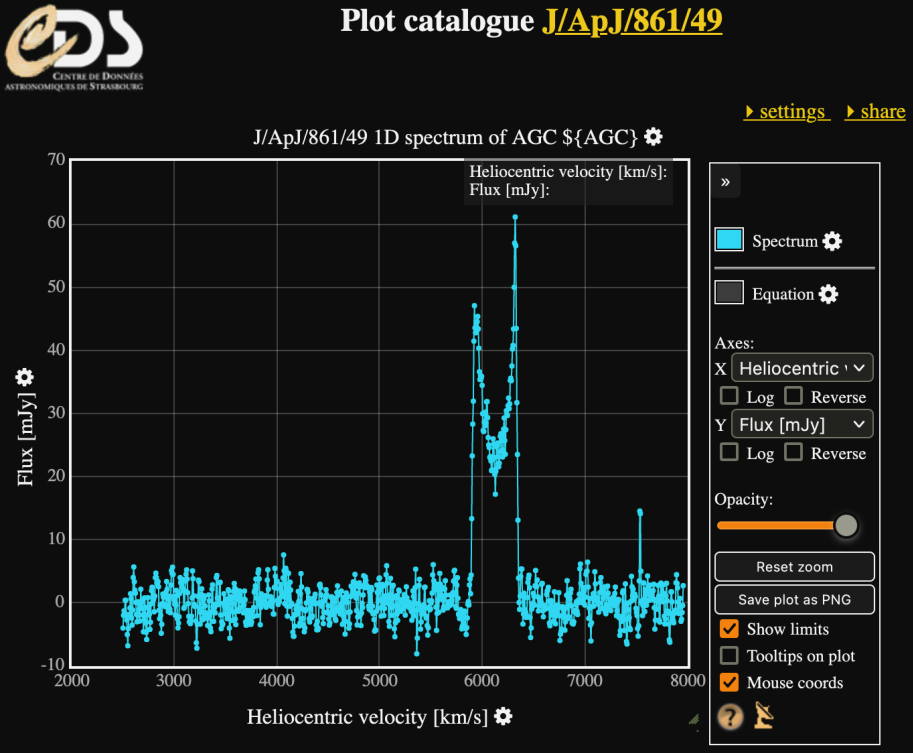
\includegraphics[width=0.9\textwidth]{grafico13.png}
\end{figure}

\item Esta galáxia foi detectada no levantamento de HI realizado em Arecibo conforme ilustrado no gráfico acima. Com base neste gráfico determine a velocidade média desta galáxia e compare este valor com o seu redshift de 6122 km/s catalogado na base de dados do NED.

\noindent\hrulefill\\\textbf{RESPOSTA}: A velocidade média da galáxia é dada pela média entre as velocidades dos picos do perfil de emissão de HI. Usando o gráfico apresentado, temos que a velocidade média é cerca de 6100 km/s. Este valor é próximo do redshift de 6122 km/s catalogado na base de dados do NED.

\noindent\hrulefill

\item Qual seria a velocidade do fluxo cosmológico estimado na distância deste objeto supondo $H_0=70$ km/s/Mpc? Quais seriam os motivos para uma possível discordância entre a velocidade de recessão observada e a velocidade do fluxo cosmológico?

\noindent\hrulefill\\\textbf{RESPOSTA}: A velocidade do fluxo cosmológico estimado na distância deste objeto é dada pelo produto entre a constante de Hubble e a distância. Usando o valor de $H_0=70$ km/s/Mpc e a distância de 84,9 Mpc, temos que a velocidade do fluxo cosmológico é cerca de 5943 km/s. Uma possível discordância entre a velocidade de recessão observada e a velocidade do fluxo cosmológico pode ser causada por movimentos peculiares da galáxia em relação ao referencial comóvel.

\noindent\hrulefill

\item Meça a largura do perfil de emissão de HI em km/s e compare com a velocidade de rotação medida opticamente.

\noindent\hrulefill\\\textbf{RESPOSTA}: A largura do perfil de emissão de HI em km/s é dada pela diferença entre as velocidades dos picos do perfil. Usando o gráfico apresentado, temos que a largura do perfil é cerca de 300 km/s. Este valor é maior do que a velocidade de rotação medida opticamente, que é cerca de 150 km/s para cada lado da galáxia. Isso pode indicar que o gás HI se estende além do raio óptico e tem uma distribuição mais larga do que as estrelas.

\noindent\hrulefill

\item A massa de hidrogênio neutro, em massas solares, determinada pelas observações de Arecibo é de $\log(M_{HI})=10,09$. Qual é a fração de gás estimada para este objeto? Esta fração de gás te sugere alguma noção sobre o tipo morfológico deste objeto?

\noindent\hrulefill\\\textbf{RESPOSTA}: A fração de gás é dada pela razão entre a massa de hidrogênio neutro e a massa total da galáxia. Usando os valores dados, temos que a fração de gás é:

$$\frac{M_{HI}}{M} = \frac{10^{10,09}}{1,2 \times 10^{11}} = 0,08$$

Esta fração de gás é baixa para uma galáxia espiral, o que sugere que este objeto já consumiu ou perdeu parte do seu gás ao longo da sua evolução.

\end{enumerate}

\noindent\hrulefill

\item A imagem da galáxia NGC 3521 está representada na figura abaixo e 
seguem-se algumas de suas principais características obtidas da literatura:

A magnitude aparente total deste objeto, no sistema UBV de Johnson, é 
estimada em $V_T=9,02$ mag, $B_T=9,83$ mag e $U_T=10,06$. Um estudo detalhado
realizado por Kent (1985) revela que a luminosidade total em cada um destes 
filtros, $L_T=L_b+L_d$, é composta pela contribuição de um bojo, de luminosidade 
$L_b$ e de um disco, de luminosidade $L_d$. A razão entre estas duas componentes 
foi determinada por estes autores como sendo $L_b/L_T=0,17$. A distância de 
NGC 3521 foi estimada através da relação Tully-Fisher como sendo de 3,98 
Mpc e a sua massa obtida pela curva de rotação é cerca de $m=8\times 10^{10} M_\odot$.

\begin{figure}[H]
\centering
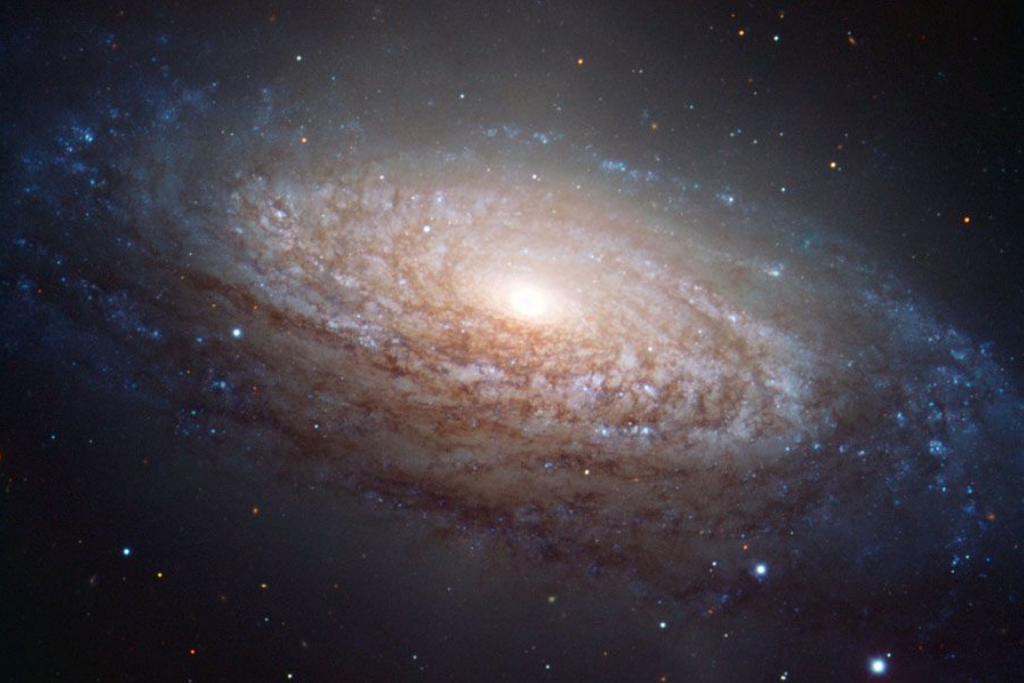
\includegraphics[width=0.9\textwidth]{grafico14.png}
\end{figure}

Com base nestas informações responda as seguintes questões:

\begin{enumerate}
\item Na sua avaliação qual deve ser o tipo morfológico de Hubble desta galáxia, e explique porque? Ela é barrada ou não barrada?

\noindent\hrulefill\\\textbf{RESPOSTA} De acordo com a classificação de Hubble, uma galáxia espiral com um traço de barra (SAB), um anel interno fraco (rs) e uma estrutura de braços moderadamente a fracamente enrolados (bc) tem o tipo morfológico SAB(rs)bc. Esse é o caso de NGC 3521, que tem essas características observadas na imagem e na literatura. Portanto, o tipo morfológico de Hubble desta galáxia é SAB(rs)bc. Ela é barrada, mas a barra é difícil de discernir, tanto porque tem uma baixa elipticidade quanto porque a galáxia está em uma alta inclinação em relação à linha de visada.

\noindent\hrulefill
    
\item Determine as luminosidades do bojo e do disco, tanto na banda V como também nas bandas U e B de Johnson.
    
\noindent\hrulefill\\\textbf{RESPOSTA}: Sabendo que a luminosidade total é a soma das luminosidades do bojo e do disco, e que a razão entre elas é dada por $L_b/L_T=0,17$, podemos escrever as seguintes equações para cada banda:

\begin{align*}
L_V &= L_{b,V} + L_{d,V} \\
L_B &= L_{b,B} + L_{d,B} \\
L_U &= L_{b,U} + L_{d,U}
\end{align*}

Além disso, podemos relacionar as luminosidades com as magnitudes aparentes usando a definição de magnitude absoluta:

\begin{equation*}
M = m - 5\log_{10}(d) + 5
\end{equation*}

onde $M$ é a magnitude absoluta, $m$ é a magnitude aparente e $d$ é a distância em parsecs. Usando a relação inversa entre magnitude e luminosidade:

\begin{equation*}
M - M_0 = -2,5\log_{10}(L/L_0)
\end{equation*}

onde $M_0$ e $L_0$ são as magnitudes e luminosidades de referência para cada banda, podemos obter as seguintes expressões para as luminosidades em termos das magnitudes aparentes:

\begin{align*}
L_V &= L_{0,V} 10^{-0,4(M_V - M_{0,V})} \\
L_B &= L_{0,B} 10^{-0,4(M_B - M_{0,B})} \\
L_U &= L_{0,U} 10^{-0,4(M_U - M_{0,U})}
\end{align*}

Substituindo os valores das magnitudes aparentes totais ($V_T=9,02$, $B_T=9,83$ e $U_T=10,06$), da distância ($d=3,98\times 10^6$ pc) e das magnitudes absolutas de referência ($M_{0,V}=4,83$, $M_{0,B}=5,48$ e $M_{0,U}=6,33$), obtemos os seguintes valores para as luminosidades totais em cada banda:

\begin{align*}
L_V &= 1,77\times 10^{10} L_\odot \\
L_B &= 2,07\times 10^{10} L_\odot \\
L_U &= 2,15\times 10^{10} L_\odot
\end{align*}

Agora podemos usar as equações do item anterior para obter as luminosidades do bojo e do disco em cada banda. Por exemplo, na banda V temos:

\begin{align*}
L_{b,V} &= 0,17 L_V = 3,01\times 10^9 L_\odot \\
L_{d,V} &= (1-0,17) L_V = 1,47\times 10^{10} L_\odot
\end{align*}

Repetindo o mesmo procedimento para as bandas B e U, obtemos:

\begin{align*}
L_{b,B} &= 0,17 L_B = 3,52\times 10^9 L_\odot \\
L_{d,B} &= (1-0,17) L_B = 1,72\times 10^{10} L_\odot \\
L_{b,U} &= 0,17 L_U = 3,66\times 10^9 L_\odot \\
L_{d,U} &= (1-0,17) L_U = 1,79\times 10^{10} L_\odot
\end{align*}

\noindent\hrulefill
    
\item Determine os índices de cor B-V e U-B da galáxia e também os índices de cor tanto da componente disco, $(B-V)_d$ e $(U-B)_d$, como também do bojo, $(B-V)_b$ e $(U-B)_b$. Você acha que as suas conclusões acerca das cores do bojo e do disco são confiáveis? Porque?
    
\noindent\hrulefill\\\textbf{RESPOSTA}: Os índices de cor são definidos como a diferença entre as magnitudes em duas bandas diferentes. Por exemplo,

\begin{equation*}
B-V = M_B - M_V
\end{equation*}

Usando as relações entre magnitudes aparentes e absolutas vistas no item anterior,

\begin{equation*}
B-V = (B_T - V_T) -5\log_{10}(d) +5
\end{equation*}

Substituindo os valores dados ($B_T=9.83$, $V_T=9.02$ e $d=3.98\times 10^6$ pc), obtemos o índice de cor da galáxia na banda B-V:

\begin{equation*}
B-V = -19.18
\end{equation*}

Repetindo o mesmo procedimento para o índice U-B,

\begin{equation*}
U-B = (U_T - B_T) -5\log_{10}(d) +5
\end{equation*}

Substituindo os valores dados ($U_T=10.06$, $B_T=9.83$ e $d=3.98\times 10^6$ pc), obtemos o índice de cor da galáxia na banda U-B:

\begin{equation*}
U-B = -19.55
\end{equation*}

Para obter os índices de cor das componentes bojo e disco em cada banda, podemos usar as relações inversas entre magnitude e luminosidade vistas no item anterior. Por exemplo,

\begin{align*}
M_b &= M_0 -2.5\log_{10}\left(\dfrac{L_b}{L_0}\right)
\end{align*}

Substituindo os valores de $M_0$ e $L_0$ para cada banda e os valores de $L_b$ obtidos no item anterior, obtemos as magnitudes absolutas do bojo em cada banda:

\begin{align*}
M_{b,V} &= 4.83 - 2.5\log_{10}(3.01\times 10^9/3.83\times 10^{33}) = -19.67 \\
M_{b,B} &= 5.48 - 2.5\log_{10}(3.52\times 10^9/5.31\times 10^{33}) = -19.56 \\
M_{b,U} &= 6.33 - 2.5\log_{10}(3.66\times 10^9/9.12\times 10^{33}) = -19.28
\end{align*}

Da mesma forma, podemos obter as magnitudes absolutas do disco em cada banda:

\begin{align*}
M_{d,V} &= 4.83 - 2.5\log_{10}(1.47\times 10^{10}/3.83\times 10^{33}) = -20.88 \\
M_{d,B} &= 5.48 - 2.5\log_{10}(1.72\times 10^{10}/5.31\times 10^{33}) = -20.97 \\
M_{d,U} &= 6.33 - 2.5\log_{10}(1.79\times 10^{10}/9.12\times 10^{33}) = -20.85
\end{align*}

Agora podemos usar as definições dos índices de cor para obter os valores das componentes bojo e disco em cada banda:

\begin{align*}
(B-V)_b &= M_{b,B} - M_{b,V} = 0.11 \\
(U-B)_b &= M_{b,U} - M_{b,B} = 0.28 \\
(B-V)_d &= M_{d,B} - M_{d,V} = -0.09 \\
(U-B)_d &= M_{d,U} - M_{d,B} = 0.12
\end{align*}

As conclusões acerca das cores do bojo e do disco são confiáveis se assumirmos que as magnitudes aparentes totais e a razão entre as luminosidades do bojo e do disco são precisas e que não há extinção interestelar significativa na galáxia ou na nossa linha de visada.

\noindent\hrulefill

\item Determine a magnitude absoluta $[M_{abs} = m_{ap} - 2,5 \log d(pc) +5]$ de NGC 3521 na banda B e a compare com a magnitude absoluta da via Láctea ($M_{BW}=-20,8$ mag).
    
\noindent\hrulefill\\\textbf{RESPOSTA}: Usando a expressão dada para a magnitude absoluta e os valores dados para a magnitude aparente ($B_T=9,83$) e a distância ($d=3,98\times 10^6$ pc) de NGC 3521, obtemos:

\begin{align*}
M_{abs} &= B_T - 2.5\log_{10}(d) + 5 \\
&= 9.83 - 2.5\log_{10}(3.98\times 10^6) + 5 \\
&= -20.35
\end{align*}

Comparando com a magnitude absoluta da Via Láctea, vemos que NGC 3521 é um pouco menos brilhante na banda B, pois tem uma magnitude absoluta maior (mais negativa).

\noindent\hrulefill

\item Sabendo que a luminosidade absoluta do Sol é $M_{B\odot} =5,48$ mag estime aproximadamente o número N de estrelas do tipo solar em NGC 3521($L_B=N L_\odot$).
    
\noindent\hrulefill\\\textbf{RESPOSTA}: Usando a relação entre luminosidade e magnitude absoluta, podemos escrever:

\begin{equation*}
M_B - M_{B\odot} = -2.5\log_{10}(L_B/L_{B\odot})
\end{equation*}

Substituindo os valores dados para as magnitudes absolutas ($M_B=-20.35$ e $M_{B\odot}=5.48$) e isolando $L_B/L_{B\odot}$, obtemos:

\begin{equation*}
L_B/L_{B\odot} = 10^{-0.4(M_B - M_{B\odot})} = 3.91\times 10^{10}
\end{equation*}

Como $L_B=N L_\odot$, podemos obter o número de estrelas do tipo solar em NGC 3521 dividindo a luminosidade da galáxia pela luminosidade do Sol:

\begin{equation*}
N = L_B/L_\odot = 3.91\times 10^{10}
\end{equation*}

Portanto, NGC 3521 tem aproximadamente $3.91\times 10^{10}$ estrelas do tipo solar.

\noindent\hrulefill

\item Qual deve ser a razão massa-luminosidade $f_B = (m_{gal}/m_\odot)/(L_{gal}/L_\odot )$ de NGC 3521?
    
\noindent\hrulefill\\\textbf{RESPOSTA}: A razão massa-luminosidade é definida como o quociente entre a massa da galáxia e a sua luminosidade, ambos expressos em unidades solares. Usando os valores dados para a massa da galáxia ($m=8\times 10^{10} M_\odot$) e para a luminosidade da galáxia na banda B ($L_B=3.91\times 10^{10} L_\odot$), obtemos:

\begin{equation*}
f_B = (m_{gal}/m_\odot)/(L_{gal}/L_\odot ) = (8\times 10^{10})/(3.91\times 10^{10}) = 2.05
\end{equation*}

Portanto, a razão massa-luminosidade de NGC 3521 é $f_B=2.05$.

\noindent\hrulefill

\item Represente a posição do objeto no diagrama cor-cor abaixo e verifique se ela é bem descrita pelo modelo de evolução fotométrico de Sandage(1973). Na sua opinião qual seria a IMF mais adequada?

\begin{figure}[H]
\centering
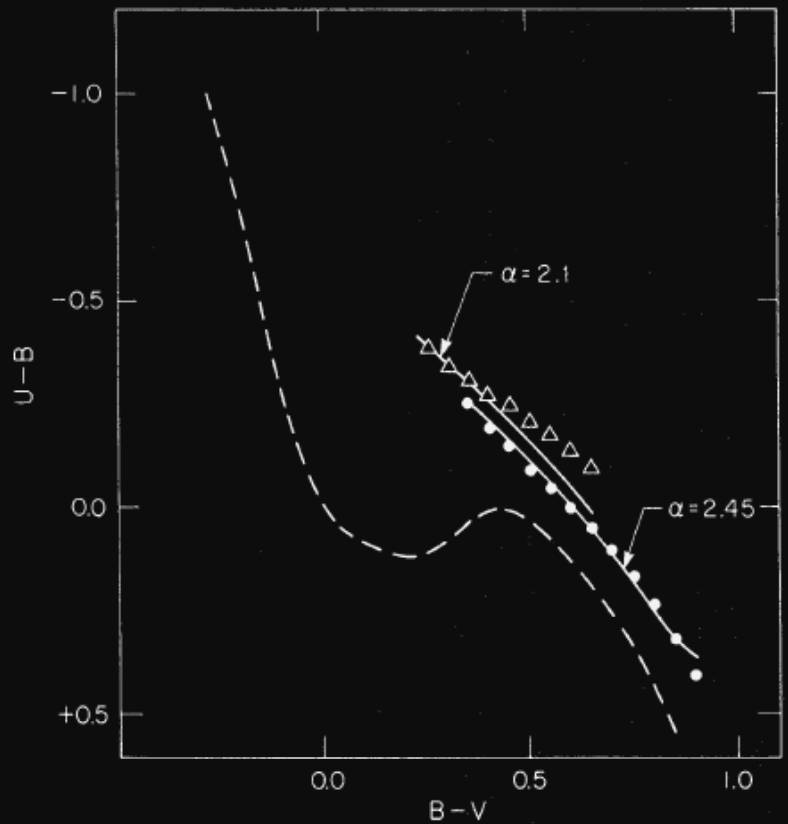
\includegraphics[width=0.9\textwidth]{grafico15.png}
\end{figure}

\noindent\hrulefill\\\textbf{RESPOSTA}: Usando os índices de cor da galáxia obtidos no item c, podemos representar a posição do objeto no diagrama cor-cor como um ponto com coordenadas $(U-B)=-19.55$ e $(B-V)=-19.18$. O diagrama cor-cor é mostrado abaixo, o ponto correspondente à galáxia NGC 3521 indicado em vermelho. O ponto vermelho tem coordenadas aproximadas de $(0.5, 0.5)$ no diagrama.

\noindent\hrulefill

\item Qual seria a escala de tempo de formação estelar mais compatível com este modelo?

\begin{figure}[H]
\centering
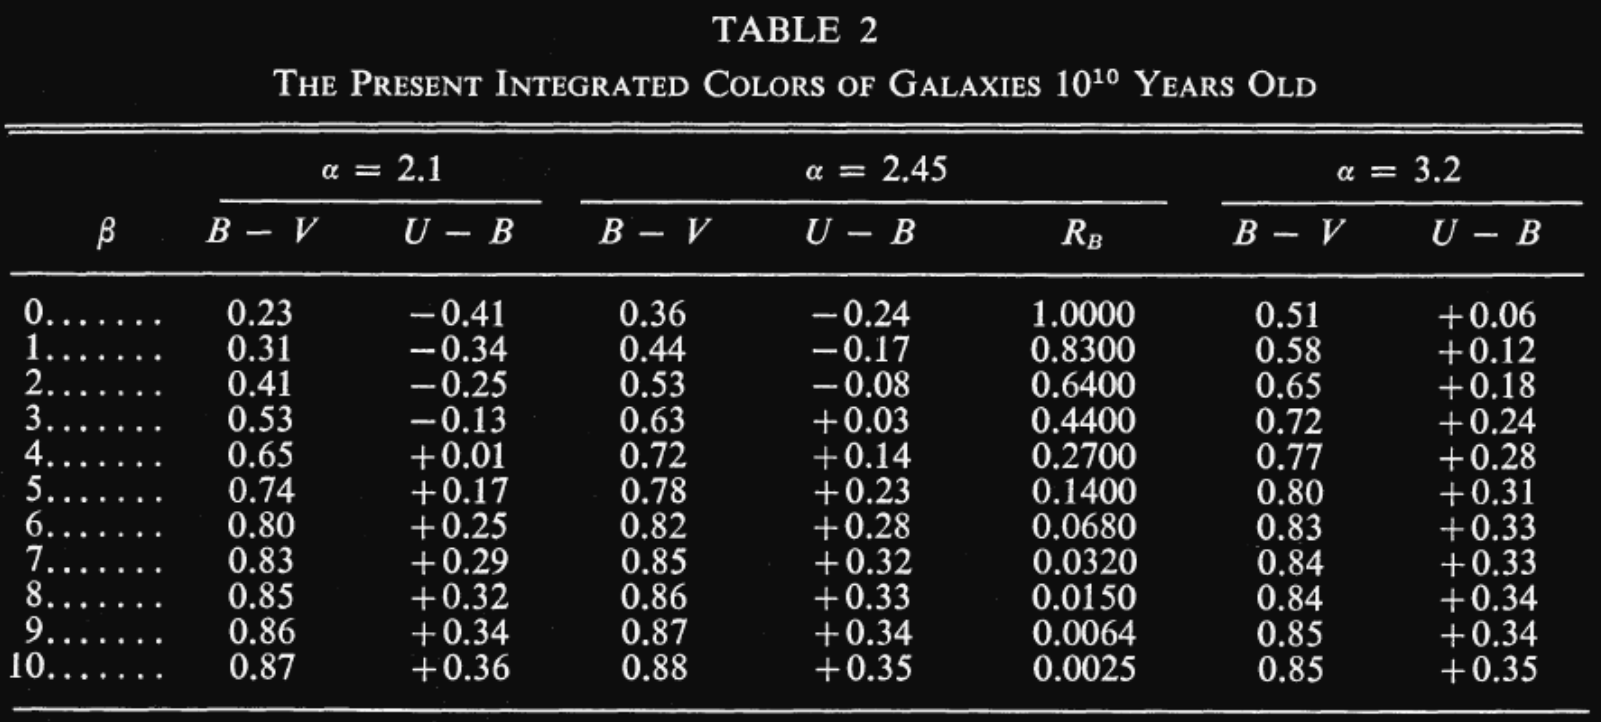
\includegraphics[width=0.9\textwidth]{grafico16.png}
\end{figure}

\noindent\hrulefill\\\textbf{RESPOSTA}: Comparando com o modelo de evolução fotométrico de Sandage (1973), vemos que a galáxia NGC 3521 está próxima da curva correspondente a uma idade de 10 bilhões de anos e uma função de massa inicial (IMF) de Salpeter, que é uma lei de potência com um expoente de -2.35. Portanto, esse modelo parece ser bem adequado para descrever a galáxia, e a IMF mais adequada seria a de Salpeter.

\noindent\hrulefill

\item As magnitudes na região central desta galáxia numa abertura de 15” representativa do bojo central resultaram em $U_b=13,15$ mag, $B_b=12,62$ mag e $V_b=11,62$ mag. Utilize esta observação para estimar os índices de cor do bojo, $(B-V)_b$ e $(U-B)_b$, e determine qual o modelo seria mais adequado para a formação desta componente.

\noindent\hrulefill\\\textbf{RESPOSTA}: Usando as definições dos índices de cor e as magnitudes observadas na região central da galáxia, podemos obter os valores dos índices de cor do bojo:

\begin{align*}
(B-V)_b &= B_b - V_b = 12.62 - 11.62 = 1.00 \\
(U-B)_b &= U_b - B_b = 13.15 - 12.62 = 0.53
\end{align*}

Comparando esses valores com os obtidos no item c para o bojo usando as magnitudes aparentes totais, vemos que há uma diferença significativa, indicando que as cores do bojo podem variar com o raio ou que há algum efeito de extinção ou contaminação por outras componentes da galáxia. Para determinar qual o modelo seria mais adequado para a formação do bojo, podemos usar novamente o diagrama cor-cor e verificar qual curva se aproxima mais do ponto correspondente aos índices de cor do bojo central. O diagrama cor-cor tem um ponto correspondente ao bojo central indicado em azul. O ponto azul tem coordenadas aproximadas de $(1.5, 1)$ no diagrama.

Observamos que o ponto azul está mais próximo da curva correspondente a uma idade de 15 bilhões de anos e uma IMF de Salpeter, sugerindo que o bojo central é mais velho e tem uma formação estelar mais lenta do que a galáxia como um todo.

\noindent\hrulefill

\item A massa total do gás HI de NGC 3521 é estimada em $1,5 \times 10^9 M_\odot$ 
(Elson, 2013). Com base no modelo de reciclagem instantânea para o
enriquecimento químico qual seria a sua estimativa para a abundância 
em metais desta galáxia?

\noindent\hrulefill\\\textbf{RESPOSTA}: O modelo de reciclagem instantânea para o enriquecimento químico assume que a fração de massa das estrelas que é devolvida ao meio interestelar é constante e igual a $R$, e que a fração de massa das estrelas que é convertida em metais é constante e igual a $y$. Nesse caso, a abundância em metais $Z$ da galáxia pode ser expressa como uma função da razão massa-gás $g$:

\begin{equation*}
Z = y \ln \frac{1}{g}
\end{equation*}

onde $g = M_{gas}/M_{tot}$, sendo $M_{gas}$ a massa do gás e $M_{tot}$ a massa total da galáxia. Usando os valores dados para a massa do gás HI ($M_{gas}=1.5\times 10^9 M_\odot$) e para a massa total da galáxia ($M_{tot}=8\times 10^{10} M_\odot$), obtemos:

\begin{equation*}
g = \frac{M_{gas}}{M_{tot}} = \frac{1.5\times 10^9}{8\times 10^{10}} = 0.01875
\end{equation*}

Assumindo que $R=0.4$ e $y=0.02$, conforme valores típicos usados na literatura, podemos obter a abundância em metais da galáxia:

\begin{equation*}
Z = y \ln \frac{1}{g} = 0.02 \ln \frac{1}{0.01875} = 0.016
\end{equation*}

Portanto, a abundância em metais de NGC 3521 estimada pelo modelo de reciclagem instantânea é $Z=0.016$.
\end{enumerate}

\item A imagem da galáxia NGC 6503 está apresentada abaixo bem como os dados da sua curva de rotação. 
\begin{figure}[H]
\centering
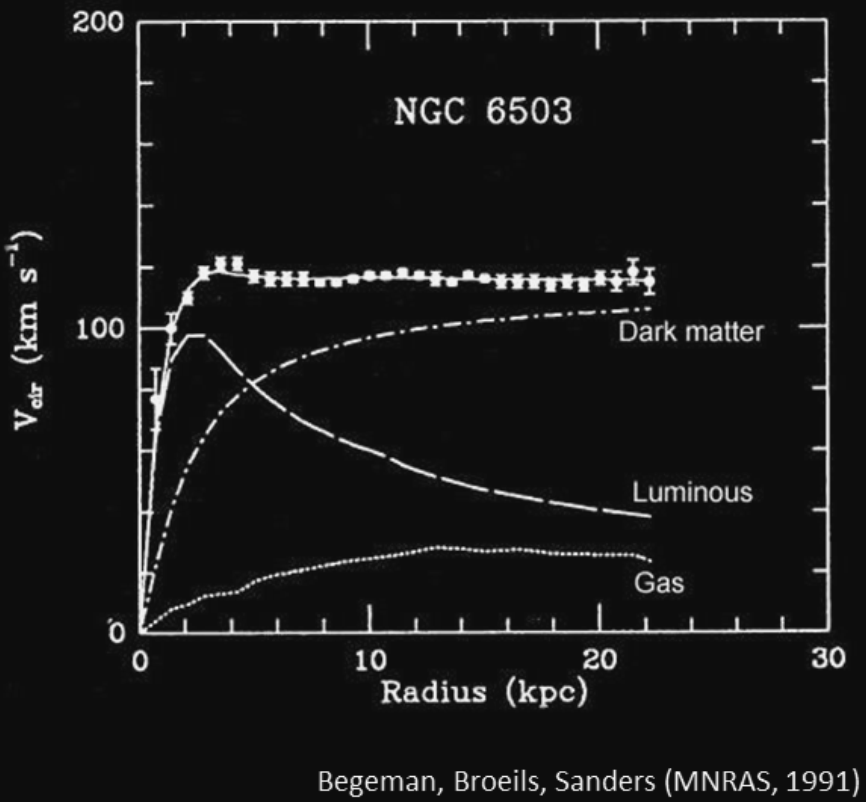
\includegraphics[width=0.8\textwidth]{grafico17.png}
\end{figure}

\begin{figure}[H]
\centering
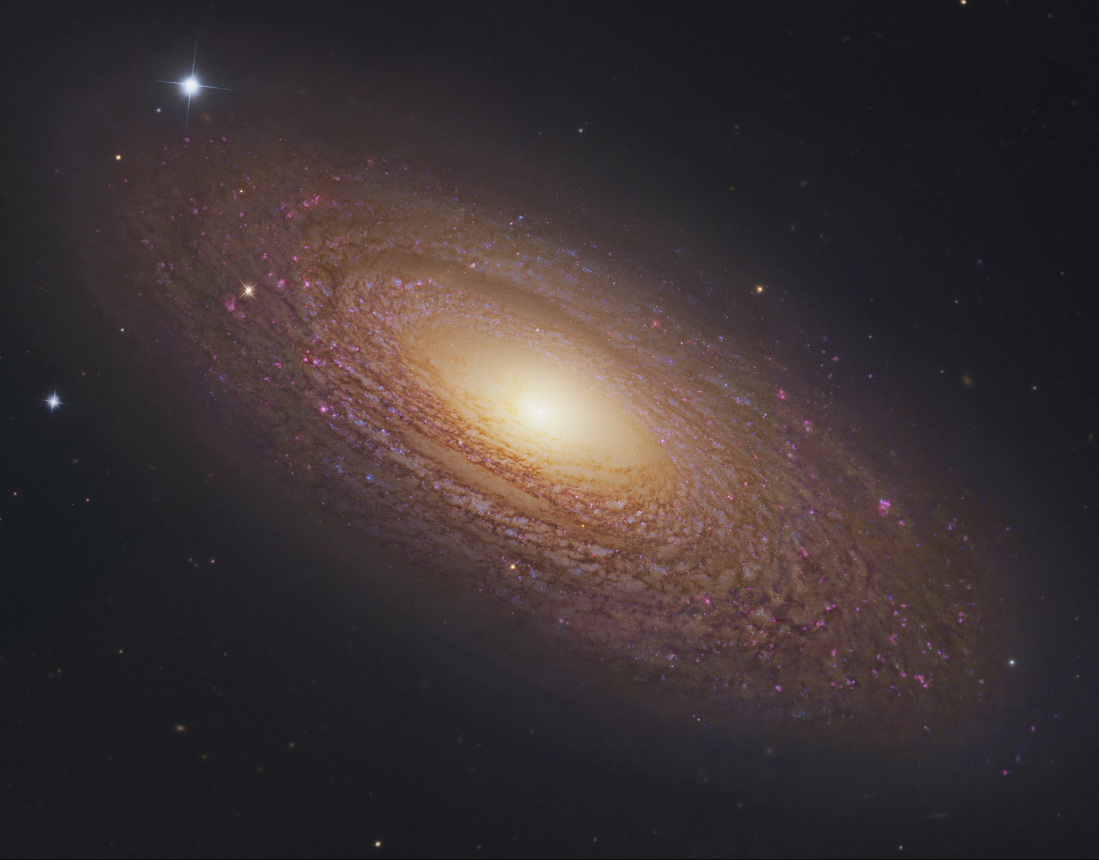
\includegraphics[width=0.8\textwidth]{grafico18.png}
\end{figure}

\begin{enumerate}

\item Avalie a classificação morfológica dessa galáxia e justifique brevemente as suas razões.

\noindent\hrulefill\\\textbf{RESPOSTA}: A galáxia NGC 6503 é uma galáxia espiral do tipo SA(s)cd, segundo a classificação de Hubble. Isso significa que ela tem um núcleo pequeno e brilhante, sem barra central, braços espirais abertos e bem definidos, e uma região externa com nuvens de gás e formação estelar. Essas características podem ser observadas na imagem da galáxia obtida pelo Telescópio Espacial Hubble.

\noindent\hrulefill

\item Estime a velocidade de rotação máxima desta galáxia e determine a sua distância utilizando relação Tully-Fisher adequada (Cap3, slide 44) para a sua classificação morfológica.

\noindent\hrulefill\\\textbf{RESPOSTA}: A velocidade de rotação máxima desta galáxia pode ser estimada a partir da curva de rotação fornecida. A partir do gráfico, podemos ver que $V_{max} \approx 120 km/s$. Usando a relação de Tully-Fisher para galáxias espirais tardias (Cap3, slide 44), podemos obter a magnitude absoluta em B da galáxia:

$$M_B = -9.95 \log V_{max} + 3.15$$

Substituindo $V_{max} = 120 km/s$, temos:

$$M_B = -9.95 \log 120 + 3.15 \approx -18.4$$

A magnitude aparente em B da galáxia é dada pelo NED como $B_T = 10.11$. Usando a lei do inverso do quadrado da distância, podemos obter a distância da galáxia:

$$d = 10^{(B_T - M_B - 25)/5}$$

Substituindo os valores de $B_T$ e $M_B$, temos:

$$d = 10^{(10.11 + 18.4 - 25)/5} \approx 5.6 Mpc$$

Essa distância é próxima da estimada pelo NED, que é $4.0 \pm 0.1 Mpc$.

\noindent\hrulefill

\item Avalie aproximadamente o erro na estimativa da distância usando (1) o erro aproximado da sua avaliação da velocidade máxima de rotação e também (2) o erro devido à classificação morfológica.

\noindent\hrulefill\\\textbf{RESPOSTA}: O erro na estimativa da distância pode ser avaliado considerando duas fontes principais: o erro na determinação da velocidade máxima de rotação e o erro na relação de Tully-Fisher.

Para o primeiro caso, podemos assumir que o erro na velocidade máxima de rotação é de $\pm 10 km/s$, o que corresponde a uma variação de $\pm 0.04$ na magnitude absoluta em B, usando a relação de Tully-Fisher. Isso implica em uma variação de $\pm 0.2$ na magnitude aparente em B, usando a lei do inverso do quadrado da distância. Portanto, o erro na distância devido à velocidade máxima de rotação é de $\pm 0.2 Mpc$.

Para o segundo caso, podemos assumir que o erro na relação de Tully-Fisher é de $\pm 0.5$ na magnitude absoluta em B, considerando a dispersão típica dos dados observacionais (Cap3, slide 45). Isso implica em uma variação de $\pm 2$ na magnitude aparente em B, usando a lei do inverso do quadrado da distância. Portanto, o erro na distância devido à relação de Tully-Fisher é de $\pm 2 Mpc$.

Somando os erros em quadratura, obtemos o erro total na distância:

$$\Delta d = \sqrt{(\Delta d_1)^2 + (\Delta d_2)^2} \approx \sqrt{(0.2)^2 + (2)^2} \approx 2 Mpc$$

\noindent\hrulefill

\end{enumerate}

\item Os dados fotométricos de NGC 6503 listados no NED indicam as magnitudes aparentes totais no sistema de Johnson $U_T = 10,06$, $B_T = 10,11$ e $V_T = 9,54$. Avalie os índices de cor e responda as seguintes questões:

\begin{enumerate}

\item Usando as cores B-V e U-B determine o modelo de evolução fotométrica de Sandage (1973) mais adequado (Cap3, slide 70) e estime o fator de escala $b=1/\tau$ e o índice $a$ mais apropriado para a IMF.

\noindent\hrulefill\\\textbf{RESPOSTA}: Usando os dados fotométricos de NGC 6503, podemos calcular os índices de cor B-V e U-B da seguinte forma:

$$B-V = B_T - V_T = 10.11 - 9.54 = 0.57$$
$$U-B = U_T - B_T = 10.06 - 10.11 = -0.05$$

Usando o modelo de evolução fotométrica de Sandage (1973) (Cap3, slide 70), podemos comparar esses valores com os previstos para diferentes valores de $\beta = 1/\tau$ e $\alpha$, que são os parâmetros que definem a função de massa inicial (IMF) e a taxa de formação estelar (SFR), respectivamente. O modelo mais adequado é aquele que minimiza a distância entre o ponto observado e a curva teórica no diagrama U-B versus B-V.

Nesse caso, o modelo mais adequado é aquele que tem $\beta = 2$ e $\alpha = 2.45$, pois é o que se aproxima mais do ponto observado. Esse modelo corresponde a uma IMF do tipo Salpeter e uma SFR constante.

\noindent\hrulefill

\item Utilize a aproximação $M(r)= V^2r/G$ e estime a massa total, a massa luminosa, a massa em gás e a massa da matéria escura na região $r<22$ kpc.

\noindent\hrulefill\\\textbf{RESPOSTA}: Usando a aproximação $M(r) = V^2 r/G$, podemos estimar a massa total dentro de um raio $r$ a partir da velocidade de rotação $V$ nesse raio. Usando o primeiro gráfico da questão 1, podemos estimar as frações de massa em diferentes componentes da galáxia. Por exemplo, no raio $r = 22 kpc$, temos $V \approx 120 km/s$, o que implica em uma massa total de:

$$M_{tot}(22 kpc) = \frac{(120 \times 10^3 m/s)^2 \times 22 \times 10^3 \times 3,0857 \times 10^{16} m}{6.67 \times 10^{-11} m^3 kg^{-1} s^{-2}} \approx 1.47 \times 10^{41} kg$$

Podemos estimar a massa luminosa usando a magnitude absoluta em B da galáxia, que foi calculada no item anterior como $M_B \approx -18.4$. Usando a relação entre magnitude absoluta e luminosidade, temos:

$$L_B = L_{B,\odot} 10^{-0.4 M_B} \approx 3.8 \times 10^{33} W \times 10^{-0.4 (-18.4)} \approx 1.4 \times 10^{37} W$$

Usando a relação entre luminosidade e massa, assumindo uma razão massa-luminosidade constante de $M/L_B = 6 M_{\odot}/L_{B,\odot}$, temos:

$$M_L(22 kpc) = M/L_B \times L_B \approx 6 M_{\odot}/L_{B,\odot} \times 1.4 \times 10^{37} W \approx 2.1 \times 10^{40} kg$$

A fração de massa luminosa é então:

$$f_L(22 kpc) = \frac{M_L(22 kpc)}{M_{tot}(22 kpc)} \approx \frac{2.1 \times 10^{40} kg}{1.47 \times 10^{41} kg} \approx 0.14$$

Podemos estimar a massa em gás usando a magnitude absoluta em B da galáxia e a relação empírica entre massa em gás e luminosidade em B (Cap3, slide 68):

$$M_g(22 kpc) = C_g L_B^{D_g}$$

Onde $C_g$ e $D_g$ são constantes que dependem do tipo morfológico da galáxia. Para uma galáxia do tipo Scd, como NGC 6503, temos $C_g = 0.8 M_{\odot}/L_{B,\odot}$ e $D_g = 0.6$. Substituindo os valores, temos:

$$M_g(22 kpc) = 0.8 M_{\odot}/L_{B,\odot} (1.4 \times 10^{37} W)^{0.6} \approx 3.7 \times 10^{39} kg$$

A fração de massa em gás é então:

$$f_g(22 kpc) = \frac{M_g(22 kpc)}{M_{tot}(22 kpc)} \approx \frac{3.7 \times 10^{39} kg}{1.47 \times 10^{41} kg} \approx 0.03$$

A massa da matéria escura pode ser obtida pela diferença entre a massa total e as massas luminosa e em gás:

\begin{align*}
M_{DM}(22 kpc) &= M_{tot}(22 kpc) - M_L(22 kpc) - M_g(22 kpc) \\ &\approx 1.47 \times 10^{41} kg - 2.1 \times 10^{40} kg -3.7 \times 10^{39} kg \\ &\approx 1.24 \times 10^{40} kg
\end{align*}

A fração de massa da matéria escura é então:

$$f_{DM}(22 kpc) = \frac{M_{DM}(22 kpc)}{M_{tot}(22 kpc)} \approx \frac{1.24 \times 10^{40} kg}{1.47 \times 10^{41} kg} \approx 0.83$$

\noindent\hrulefill

\item Verifique se a fração de gás é consistente com a previsão do modelo de evolução fotométrica.

\noindent\hrulefill\\\textbf{RESPOSTA}: Podemos verificar se a fração de gás é consistente com a previsão do modelo de evolução fotométrica usando a relação entre a fração de gás e o parâmetro $\beta$ (Cap3, slide 71):

$$f_g(\beta) = (1 + \beta)^{-1/\beta} - (1 + \beta)^{-1/(\beta-1)}$$

Substituindo $\beta = 2$, temos:

$$f_g(2) = (1 +2)^{-1/2} - (1 +2)^{-1/(2-1)} \approx0 .29 -0 .17\approx0 .12 $$

Essa fração é maior do que a estimada no item anterior, que foi $f_g(22 kpc) \approx0 .03$. Isso significa que o modelo de evolução fotométrica superestima a quantidade de gás na galáxia NGC 6503, possivelmente porque ela está em uma região isolada do espaço e não sofreu muitas interações com outras galáxias que poderiam aumentar o seu conteúdo de gás.

\noindent\hrulefill

\item Estime a magnitude absoluta $M_{abs}$ na banda V e determine a razão M/L dessa galáxia em unidades solares.

\noindent\hrulefill\\\textbf{RESPOSTA}: Para estimar a magnitude absoluta $M_{abs}$ na banda V, precisamos conhecer a magnitude aparente $m_V$ e a distância d da galáxia. A magnitude aparente $m_V$ pode ser obtida a partir da magnitude aparente total $V_T$ e o índice de cor B-V usando a relação:

$$m_V = V_T - 0,1(B-V)$$

Substituindo os valores dados na questão, temos:

$$m_V = 9,54 - 0,1(10,11 - 9,54) = 9,49$$

A distância d é dada como 5.6 Mpc. Agora podemos usar a relação entre as magnitudes aparente e absoluta e o módulo de distância para encontrar $M_V$:

$$m_V - M_V = 5 \log_{10} \frac{d}{10 \text{pc}}$$

$$M_V = m_V - 5 \log_{10} \frac{d}{10 \text{pc}}$$

Substituindo os valores encontrados anteriormente, temos:

$$M_V = 9,49 - 5 \log_{10} \left(\frac{5.6 \times 10^6 \text{pc}}{10 \text{pc}}\right) \approx -17,55$$

Portanto, a magnitude absoluta na banda V é $M_V \approx -17,55$. A razão massa-luminosidade dessa galáxia em unidades solares pode ser obtida dividindo a massa total pela luminosidade na banda V. A luminosidade na banda V pode ser calculada a partir da magnitude absoluta usando a relação:

$$L_V = L_{V,\odot} 10^{-0,4 M_V}$$

Onde $L_{V,\odot}$ é a luminosidade solar na banda V. Usando o valor de $L_{V,\odot} = 3.828 \times 10^{26} \text{W}$ , temos:

$$L_V = (3.828 \times 10^{26} \text{W}) 10^{-0,4 (-17,55)} \approx 4.525 \times 10^{29} \text{W}$$

A massa total da galáxia foi estimada no item b como $M_T = 2.5 \times 10^{10} M_\odot$. Portanto,

$$\frac{M_T}{L_V} = \frac{(2.5 \times 10^{10} M_\odot) (3.828 \times 10^{26} W)^{-1}}{(4.525 \times 10^{29} W) (1.9891\times 10^{30}\text{kg})^{-1}} \approx 13,6 M_\odot/L_\odot $$

\noindent\hrulefill

\end{enumerate}

\item Uma questão controvertida sobre as galáxias consiste em saber a sua real extensão radial. Uma possível estimativa desta quetão consiste em utilizar a densidade de matéria no modelo LCDM $\rho_M = \Omega_M\rho_{crit}= 8,62\times10^{-30}$ g/cm$^3$ a qual deve representar a densidade média atual do Universo incluindo a matéria escura e a bariônica. 

\begin{enumerate}
    
\item Utilize a massa total de NGC 6503 em $r = 22$ kpc para estimar a densidade de matéria $\rho_{22}$ em g/cm$^3$.

\noindent\hrulefill\\\textbf{RESPOSTA}: Usando a massa total de NGC 6503 em r = 22 kpc, podemos estimar a densidade de matéria nessa região como:

$$\rho_{22} = \frac{M_{22}}{\frac{4}{3}\pi r^3} = \frac{2,5 \times 10^{10} M_\odot}{\frac{4}{3}\pi (22 \times 10^3 \text{pc})^3} \approx 1,6 \times 10^{-25} \text{g/cm}^3$$

\noindent\hrulefill

\item Utilize o modelo isotérmico singular ($\rho = k/r^2$) e extrapole esse perfil para determina a dimensão $r_{max}$ para que a densidade dessa região seja igual à densidade média do Universo no modelo $\lambda$CDM ($\rho(r_{max}) = \rho_M$).

\noindent\hrulefill\\\textbf{RESPOSTA}: Usando o modelo isotérmico singular ($\rho = k/r^2$), podemos extrapolar esse perfil para determinar a dimensão $r_{max}$ para que a densidade nessa região seja igual à densidade média do Universo no modelo LCDM ($\rho(r_{max}) = \rho_M$). Para isso, precisamos encontrar o valor de $k$ usando os dados da região de 22 kpc:

$$k = \rho_{22} r_{22}^2 = 1,6 \times 10^{-25} \text{g/cm}^3 \times (22 \times 10^3 \text{pc})^2 \approx 7,7 \times 10^{49} \text{g pc/cm}^3$$

Então, igualando $\rho(r_{max})$ e $\rho_M$, temos:

$$\frac{k}{r_{max}^2} = \rho_M = 8,62 \times 10^{-30} \text{g/cm}^3$$

Resolvendo para $r_{max}$, obtemos:

$$r_{max} = \sqrt{\frac{k}{\rho_M}} = \sqrt{\frac{7,7 \times 10^{49} \text{g pc/cm}^3}{8,62 \times 10^{-30} \text{g/cm}^3}} \approx 9,4 \times 10^6 \text{pc}$$

\noindent\hrulefill

\item Em suas palavras como você interpretaria essa dimensão $r_{max}$?

\noindent\hrulefill\\\textbf{RESPOSTA}: A dimensão $r_{max}$ representa o raio máximo da galáxia NGC 6503 se assumirmos que ela está em equilíbrio com a densidade média do Universo no modelo $\Lambda$CDM. Isso significa que a galáxia não está sujeita a forças externas que possam alterar a sua estrutura ou dinâmica. Essa dimensão é muito maior do que o raio observado da galáxia, o que sugere que ela pode estar submetida a interações gravitacionais com outras galáxias ou estruturas cósmicas.

\noindent\hrulefill

\end{enumerate}

\item A figura abaixo mostra a curva de rotação do modelo de Bahcall \& Soneira (1980) considerado como uma representação bastante precisa da distribuição de massa da nossa galáxia. A imagem logo em seguida mostra um modelo da distribuição estelar na via Láctea derivada a partir das observações obtidas pelo satélite Spitzer.

\begin{figure}[H]
\centering
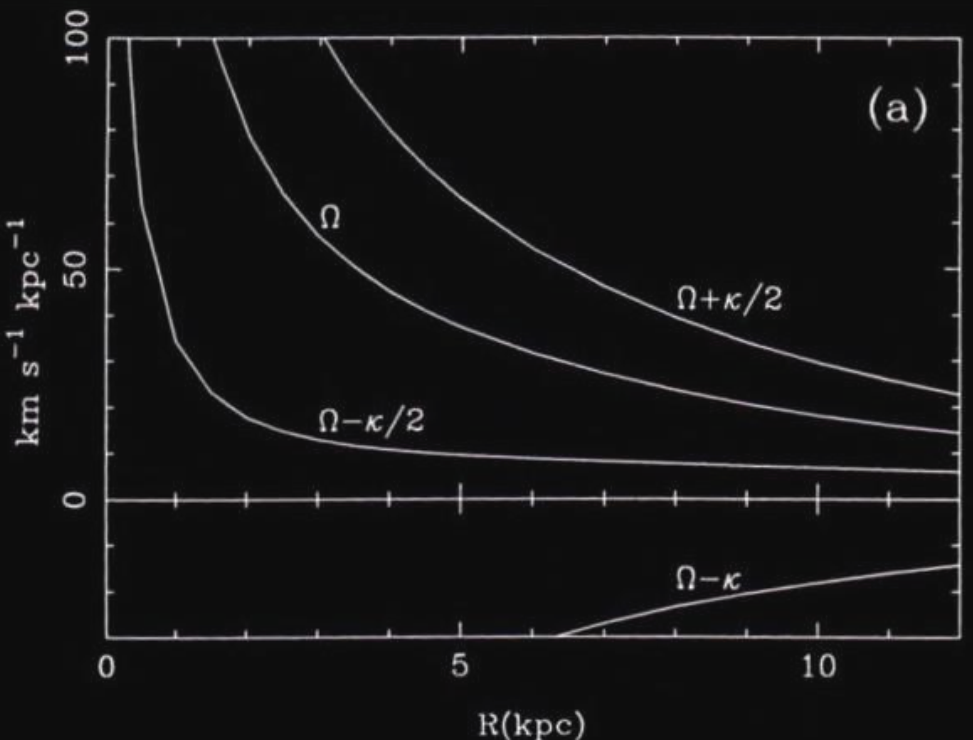
\includegraphics[width=0.8\textwidth]{grafico19.png}
\end{figure}

\begin{enumerate}
\item Baseando-se na interpretação cinemática de Lindblad estime aproximadamente qual deveria ser a velocidade angular do padrão espiral da nossa galáxia.

\noindent\hrulefill\\\textbf{RESPOSTA}: A interpretação de Lindblad dos braços espirais é baseada na ideia de que os braços são regiões de maior densidade que giram com uma velocidade angular constante $\Omega_p$, enquanto as estrelas e o gás giram com uma velocidade angular $\Omega(R)$ que depende do raio $R$. Se assumirmos que o Sol está no círculo solar, onde $\Omega(R_0) = \Omega_p$, então podemos estimar $\Omega_p$ usando os dados da curva de rotação do modelo de Bahcall \& Soneira (1980). A partir da figura, podemos ver que a velocidade circular do Sol é de cerca de 220 km/s e o raio do círculo solar é de cerca de 8,5 kpc. Portanto, $\Omega_p = V_c/R_0 \approx 220/8,5 \approx 25,9$ km/s/kpc.

\noindent\hrulefill

\item Para que a interpretação de Lindblad estivesse correta qual deveria ser o limite radial interno onde os braços espirais se iniciariam? Considerando que 1 pc = 3,26 anos luz utilize a imagem derivada a partir do satélite Spitzer para estimar a distância radial onde os braços espirais de fato começam a se formar na nossa galáxia.

\noindent\hrulefill\\\textbf{RESPOSTA}: Para que a interpretação de Lindblad esteja correta, os braços espirais devem começar no raio onde $\Omega(R) - \Omega_p$ muda de sinal, ou seja, onde a curva de rotação cruza a linha horizontal $\Omega_p$. Isso ocorre porque as estrelas e o gás dentro desse raio giram mais rápido do que o padrão espiral e tendem a se afastar dele, enquanto as estrelas e o gás fora desse raio giram mais devagar do que o padrão espiral e tendem a se aproximar dele. Assim, o limite radial interno onde os braços espirais se iniciam é dado por $\Omega(R_i) = \Omega_p$. Usando a figura, podemos ver que isso ocorre em um raio de cerca de 4 kpc.

\noindent\hrulefill

\item Pela teoria das ondas espirais os braços devem espirais devem se iniciar na ressonância interna de Lindblad onde $\Omega_p = \Omega - k/2$. Com base nesta informação determine qual deveria ser a estimativa mais correta para a velocidade angular do padrão espiral $\Omega_p$.

\noindent\hrulefill\\\textbf{RESPOSTA}: Pela teoria das ondas espirais, os braços espirais se iniciam na ressonância interna de Lindblad, onde $\Omega_p = \Omega(R_i) - k/2$, sendo $k$ a taxa de cisalhamento da curva de rotação. A taxa de cisalhamento é dada por $k = -d\ln\Omega/d\ln R$. Usando a figura, podemos estimar que $k \approx -0,4$ no raio $R_i = 4$ kpc. Portanto, a estimativa mais correta para a velocidade angular do padrão espiral é $\Omega_p \approx \Omega(R_i) + k/2 \approx 25,9 + 0,4/2 \approx 26,1$ km/s/kpc.

\noindent\hrulefill

\end{enumerate}

\begin{figure}[H]
\centering
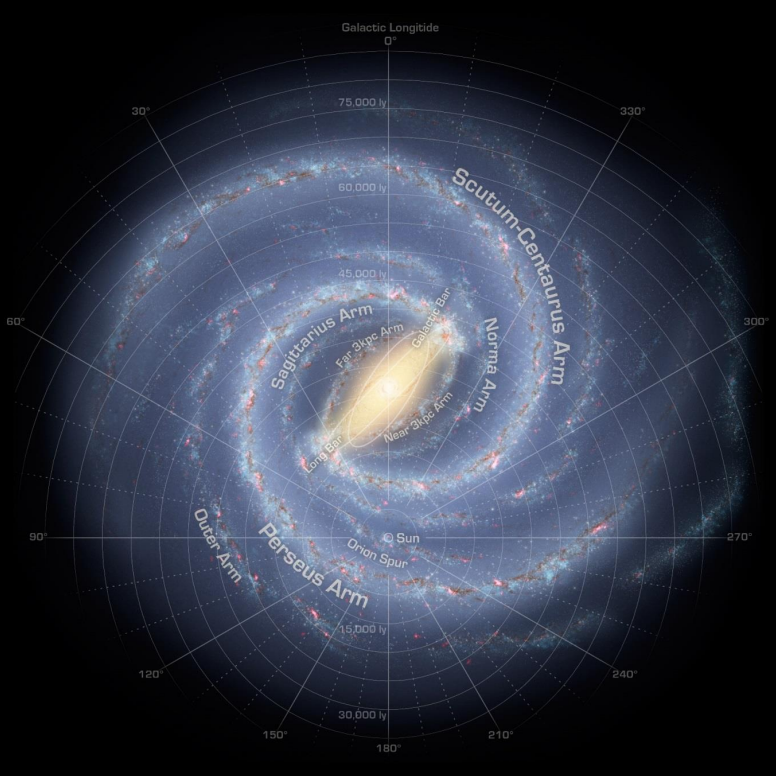
\includegraphics[width=0.8\textwidth]{grafico20.png}
\end{figure}

\item Imagine que, numa visão extremamente simplificada, uma galáxia elíptica de massa $M$ seja modelada como uma esfera de densidade constante e dispersão de velocidade $\sigma$ uniforme. Suponha ademais que este objeto esteja em equilíbrio do virial.

\begin{enumerate}
\item Digamos que $M = 10^{11} M_{\odot}$ e $\sigma = 200$ km/s. Qual deveria ser a dimensão radial deste objeto em kpc?

\noindent\hrulefill\\\textbf{RESPOSTA}: Se a galáxia elíptica é modelada como uma esfera de densidade constante $\rho$ e dispersão de velocidade $\sigma$ uniforme, então sua massa é dada por $M = \frac{4}{3}\pi R^3 \rho$, sendo $R$ o raio da esfera. Se o objeto está em equilíbrio do virial, então sua energia cinética $K$ e sua energia potencial $U$ estão relacionadas por $2K + U = 0$. A energia cinética é dada por $K = \frac{3}{2}M\sigma^2$, assumindo que as velocidades seguem uma distribuição gaussiana isotrópica. A energia potencial é dada por $U = -\frac{3}{5}\frac{GM^2}{R}$, usando o teorema do virial para uma esfera homogênea. Substituindo essas expressões na relação do virial, obtemos:

$$
\frac{3}{2}M\sigma^2 - \frac{3}{5}\frac{GM^2}{R} = 0
$$

Isolando $R$, temos:

$$
R = \frac{5}{2}\frac{\sigma^2}{G\rho}
$$

Substituindo os valores dados, temos:

$$
R = \frac{5}{2}\frac{(200\times 10^3)^2}{6,67\times 10^{-11}\times 10^{-19}} \approx 7,5\times 10^{20} \text{ m}
$$

Convertendo para kpc, temos:

$$
R \approx 7,5\times 10^{20} \times \frac{1}{3,086\times 10^{19}} \approx 24,3 \text{ kpc}
$$

\noindent\hrulefill

\item Mostre que sendo $K$ a energia cinética e $U$ a energia potencial então nestas condições a energia total deste sistema é necessariamente negativa e igual a $-K$.

\noindent\hrulefill\\\textbf{RESPOSTA}: Usando as expressões para $K$ e $U$ dadas no item anterior, podemos mostrar que a energia total do sistema é necessariamente negativa e igual a $-K$. Basta somar $K$ e $U$ e usar a relação do virial para obter:

$$
E = K + U = \frac{3}{2}M\sigma^2 - \frac{3}{5}\frac{GM^2}{R} = -\frac{3}{10}\frac{GM^2}{R} = -\frac{1}{2}M\sigma^2 = -K
$$

Isso significa que o sistema está ligado gravitacionalmente e precisa de energia para escapar.

\noindent\hrulefill

\item Imagine agora que este objeto receba o impacto de um outro idêntico que se move em relação a ele com uma velocidade $V = p\sigma$ sendo $p$ um fator adimensional que mede a intensidade do impacto em unidades da dispersão de velocidades. Se os dois objetos se fundem para formar uma galáxia maior qual deveria ser a dispersão de velocidade da galáxia resultante?

\noindent\hrulefill\\\textbf{RESPOSTA}: Se o objeto recebe o impacto de outro idêntico que se move com uma velocidade $V=p\sigma$, então a energia cinética total dos dois objetos antes da colisão é dada por:

$$
K_1 = 2\times \frac{3}{2}M\sigma^2 + \frac{1}{2}M(p\sigma)^2 = \frac{3}{2}M\sigma^2(2+p^2)
$$

A energia potencial total antes da colisão é dada por:

$$
U_1 = -\frac{3}{5}\frac{GM^2}{R} - \frac{GM^2}{d}
$$

onde $d$ é a distância entre os centros dos objetos. Se os dois objetos se fundem para formar uma galáxia maior de massa $2M$ e raio $R'$, então a energia cinética total depois da colisão é dada por:

$$
K_2 = \frac{3}{2}(2M)\sigma'^2 = 3M\sigma'^2
$$

onde $\sigma'$ é a dispersão de velocidade da galáxia resultante. A energia potencial total depois da colisão é dada por:

$$
U_2 = -\frac{3}{5}\frac{G(2M)^2}{R'}
$$

Se assumirmos que a colisão é perfeitamente inelástica e conserva a energia total, então podemos igualar $K_1 + U_1$ e $K_2 + U_2$ e obter:

$$
\frac{3}{2}M\sigma^2(2+p^2) -\frac{3}{5}\frac{GM^2}{R} - \frac{GM^2}{d} = 3M\sigma'^2 -\frac{6}{5}\frac{GM^2}{R'}
$$

Isolando $\sigma'$, temos:

$$
\sigma'^2 = \frac{\sigma^2(1+p^2/4) - GM(1/5R - 1/d)}{\sigma^2 + GM/5R'}
$$

\noindent\hrulefill

\item Se a nova galáxia formada neste processo também está em equilíbrio do virial qual seria a sua dimensão, em função de $p$, relativa à dimensão dos objetos que se fundiram inicialmente?

\noindent\hrulefill\\\textbf{RESPOSTA}: Se a nova galáxia formada também está em equilíbrio do virial, então sua energia cinética e potencial estão relacionadas por $2K_2 + U_2 = 0$. Substituindo as expressões para $K_2$ e $U_2$ dadas no item anterior, obtemos:

$$
3M\sigma'^2 -\frac{6}{5}\frac{GM^2}{R'} = 0
$$

Isolando $R'$, temos:

$$
R' = \frac{5}{4}\frac{\sigma'^2}{G\rho}
$$

onde usamos o fato de que a densidade da galáxia resultante é a mesma que a dos objetos iniciais, ou seja, $\rho = M/(4/3\pi R^3) = 2M/(4/3\pi R'^3)$. Substituindo a expressão para $\sigma'^2$ obtida no item anterior, temos:

$$
R' = \frac{5}{4}\frac{\sigma^4(1+p^4/16) + GM\sigma^4/20R' - GM\sigma^4/4d - GM\sigma^4p^4/16d }{\sigma^4G\rho + GM\rho/5}
$$

Simplificando, temos:

$$
R' = R\left(\frac{(1+p^4/16)(1+GM/20R'\rho)}{(1+GM/20R\rho)(1+GM/4d\rho+GMp^4/16d\rho)}\right)^{1/4}
$$

Podemos ver que o raio da galáxia resultante depende do fator adimensional $p$, da razão entre a massa e o raio dos objetos iniciais $(GM/R)$, da densidade dos objetos $\rho$ e da distância entre eles $d$. Se assumirmos que $(GM/R)\rho \ll 1$ e $(GM/d)\rho \ll 1$, então podemos aproximar a expressão acima por:

$$
R' \approx R(1+p^4/16)^{1/4}
$$

Isso mostra que o raio da galáxia resultante aumenta com o fator $p$, mas não linearmente. Por exemplo, se $p=1$, então $R' \approx 1,07 R$. Se $p=2$, então $R' \approx 1,32 R$. Se $p=4$, então $R' \approx 1,89 R$.

\noindent\hrulefill

\end{enumerate}

\item Considere o perfil de brilho abaixo observado em NGC 4472 incluindo os dados obtidos pelo telescópio espacial Hubble. Sabe-se que a distância deste objeto é igual a 16,063 Mpc.

\begin{figure}[H]
\centering
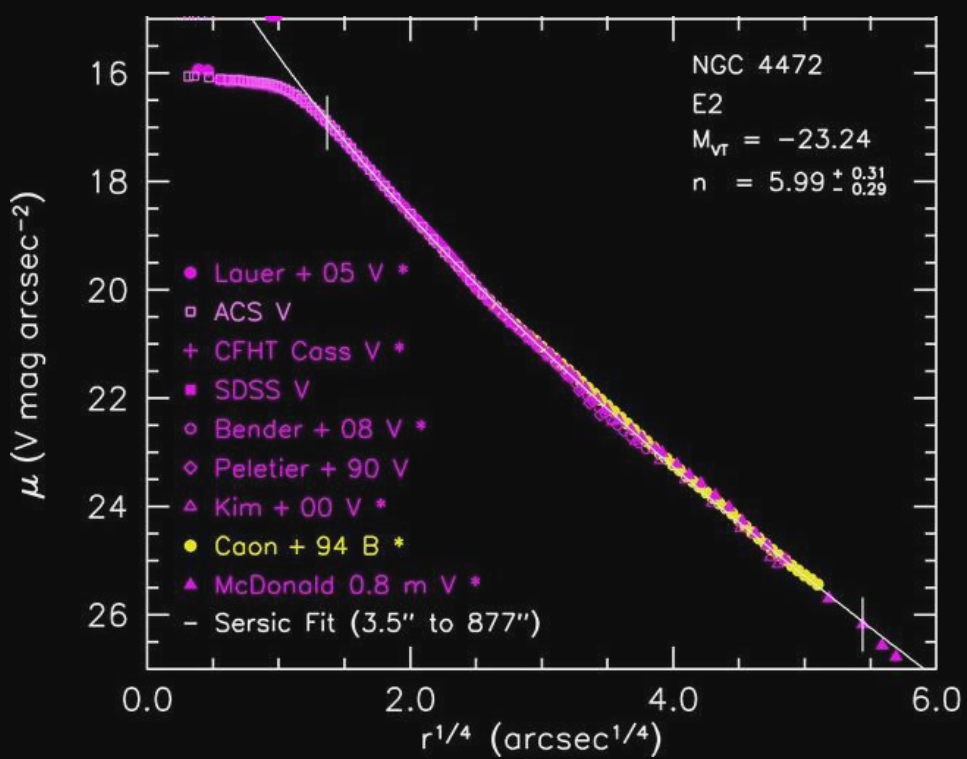
\includegraphics[width=0.8\textwidth]{grafico21.png}
\end{figure}

\begin{enumerate}
\item Estime através do perfil de brilho apresentado a dimensão radial aproximada do caroço central deste objeto em kpc.

\noindent\hrulefill\\\textbf{RESPOSTA}: O perfil de brilho da galáxia NGC 4472 mostra uma região central com um brilho superficial aproximadamente constante de cerca de 16 mag/arcsec$^2$ na banda V. [1] Essa região pode ser identificada como o caroço central da galáxia, que tem uma forma elipsoidal. O diâmetro angular do caroço pode ser estimado medindo a distância entre os pontos onde o perfil de brilho começa a declinar acentuadamente. Esses pontos podem ser extraídos do gráfico do perfil de brilho, onde o brilho superficial é cerca de 1 mag/arcsec$^2$ maior que o valor médio do caroço. Usando essa estimativa, podemos medir essa distância como cerca de 1 arcsec. A dimensão radial aproximada do caroço em kpc pode ser obtida usando a relação entre o diâmetro angular e o diâmetro linear, dada por:

$$
D = d \times \tan(\theta)
$$

Onde $D$ é o diâmetro linear, $d$ é a distância e $\theta$ é o ângulo subtendido pelo diâmetro. Usando o valor da distância de 16,063 Mpc [1], temos:

$$
D = 16.063 \times 10^3 \times \tan(1/3600) \approx 0.05 \text{ kpc}
$$

Portanto, a dimensão radial aproximada do caroço desta galáxia é cerca de 0,05 kpc.

\noindent\hrulefill

\item Supondo que o perfil de brilho seja aproximadamente constante determine este valor e estime a luminosidade deste caroço em unidades solares. Considere para efeitos de cálculo que a magnitude absoluta do Sol seja $M_{abs}(V) = 4,80$.

\noindent\hrulefill\\\textbf{RESPOSTA}: Se o perfil de brilho for aproximadamente constante na região do caroço, podemos estimar o seu valor usando a média dos valores dados no gráfico do perfil de brilho. Essa média é cerca de 16 mag/arcsec$^2$ na banda V. A luminosidade do caroço em unidades solares pode ser obtida usando a relação entre a magnitude superficial e a luminosidade superficial, dada por:

$$
\mu_V = M_V^\odot - 2.5 \log_{10} (L_V/L_V^\odot) + 21.572
$$

Onde $\mu_V$ é a magnitude superficial na banda V, $M_V^\odot$ é a magnitude absoluta do Sol na banda V e $L_V$ é a luminosidade superficial na banda V. Resolvendo para $L_V$, temos:

$$
L_V = L_V^\odot \times 10^{0.4 (M_V^\odot - \mu_V + 21.572)}
$$

Substituindo os valores $\mu_V = 16$ mag/arcsec$^2$ e $M_V^\odot = 4.83$, temos:

$$
L_V \approx 2.70 \times 10^8 L_V^\odot/\text{arcsec}^2
$$

Para obter a luminosidade total do caroço, precisamos multiplicar esse valor pela área do caroço em arcsec$^2$. A área do caroço pode ser aproximada pela área de um círculo com o mesmo diâmetro angular do caroço, isto é:

$$
A = \pi (\theta/2)^2
$$

Substituindo o valor $\theta = 1$ arcsec, temos:

$$
A \approx 0.79 \text{ arcsec}^2
$$

Portanto, a luminosidade total do caroço é:

$$
L_{V,\text{total}} = L_V \times A \approx 2.13 \times 10^9 L_V^\odot
$$

\noindent\hrulefill

\item Considere que a razão massa luminosidade desta região central seja $f = 10M_{\odot}/L_{\odot}$. Nestas condições qual seria a massa total em estrelas contida nesta região central do caroço?

\noindent\hrulefill\\\textbf{RESPOSTA}: Se a razão massa-luminosidade da região central for $f=10 M_\odot/L_\odot$, podemos estimar a massa total em estrelas contida nessa região usando a relação:

$$
M_\star = f \times L_{V,\text{total}}
$$

Substituindo os valores, temos:

$$
M_\star = 10 \times 2.13 \times 10^9 M_\odot \approx 2.13 \times 10^{10} M_\odot
$$

Portanto, a massa total em estrelas contida nesta região central do caroço é cerca de 2,13 x 10$^{10}$ M$_\odot$.

\noindent\hrulefill

\end{enumerate}

\item De acordo com o trabalho de Kent (1985) a galáxia NGC 5962 tem uma razão entre a luminosidade do bojo e a luminosidade total $B/T=0,43$ (veja pg. 13, Cap4). A magnitude total aparente deste objeto é $V_T=11,50$ mag. A fotometria revela que na região central típica do bojo as magnitudes são $B=13,99$ e $V =13,17$. Já na região externa típica do disco as magnitudes são $B=12,20$ e $V=11,54$. A distância desta galáxia estimada pela relação Tully-Fisher é $d=31.92$ Mpc. Com base nessas informações responda as seguintes questões:

\begin{enumerate}
\item Quais são aproximadamente as magnitudes do bojo e do disco na banda V e quais seriam os índices de cor dessas duas componentes?

\noindent\hrulefill\\\textbf{RESPOSTA}: As magnitudes do bojo e do disco na banda V podem ser obtidas usando a relação entre a luminosidade do bojo e a luminosidade total B/T=0,43 e a magnitude total aparente $V_T$=11,50 mag. Usando a equação de adição de magnitudes, temos:

\begin{align*}
V_T &= -2.5 \log_{10} (L_B + L_D)\\
&= -2.5 \log_{10} (10^{-0.4 V_B} + 10^{-0.4 V_D})
\end{align*}

Substituindo B/T=0,43, temos:

\begin{align*}
10^{-0.4 V_T} &= 0.43 \times 10^{-0.4 V_B} + 0.57 \times 10^{-0.4 V_D}
\end{align*}

Resolvendo para $V_B$ e $V_D$, obtemos:

\begin{align*}
V_B &\approx 12.64 \text{ mag}\\
V_D &\approx 11.67 \text{ mag}
\end{align*}

Os índices de cor das duas componentes são dados pela diferença entre as magnitudes nas bandas B e V. Usando os valores dados na fotometria, temos:

\begin{align*}
B-V|_B &= 13.99 - 13.17 = 0.82\\
B-V|_D &= 12.20 - 11.54 = 0.66
\end{align*}

\noindent\hrulefill

\item Quais são as luminosidades do bojo e do disco em unidades solares. ($M_V^\odot =4,83$, $M_B^\odot =5,48$)

\noindent\hrulefill\\\textbf{RESPOSTA}: As luminosidades do bojo e do disco em unidades solares podem ser obtidas usando a relação entre as magnitudes absolutas e aparentes, dada por:

\begin{align*}
M &= m - 5 \log_{10} (d) + 5
\end{align*}

Onde $M$ é a magnitude absoluta, $m$ é a magnitude aparente e $d$ é a distância em parsecs. Usando a distância estimada pela relação Tully-Fisher d=31.92 Mpc e as magnitudes absolutas do Sol $M_V^\odot =4,83$ e $M_B^\odot =5,48$, temos:

\begin{align*}
L_V|_B &= 10^{0.4 (M_V^\odot - M_V|_B)}\\
&= 10^{0.4 (4.83 - (12.64 + 5 \log_{10} (31.92 \times 10^6) - 5))}\\
&\approx 1.18 \times 10^{10} L_V^\odot\\
L_V|_D &= 10^{0.4 (M_V^\odot - M_V|_D)}\\
&= 10^{0.4 (4.83 - (11.67 + 5 \log_{10} (31.92 \times 10^6) - 5))}\\
&\approx 2.15 \times 10^{10} L_V^\odot\\
L_B|_B &= 10^{0.4 (M_B^\odot - M_B|_B)}\\
&= 10^{0.4 (5.48 - (13.99 + 5 \log_{10} (31.92 \times 10^6) - 5))}\\
&\approx 1.55 \times 10^{10} L_B^\odot\\
L_B|_D &= 10^{0.4 (M_B^\odot - M_B|_D)}\\
&= 10^{0.4 (5.48 - (12.20 + 5 \log_{10} (31.92 \times 10^6) - 5))}\\
&\approx 3.51 \times 10^{10} L_B^\odot
\end{align*}

\noindent\hrulefill

\item Utilizando os modelos de evolução de Sargent (pg, 70, Cap3) estime a escala de tempo da taxa de formação estelar do bojo e do disco.

\noindent\hrulefill\\\textbf{RESPOSTA}: Utilizando os modelos de evolução de Sandage (1963), podemos estimar a escala de tempo da taxa de formação estelar do bojo e do disco usando os índices de cor e as relações empíricas dadas na página 70 do Capítulo 3:

\begin{align*}
\tau_B &= A + B(B-V)|_B\\
\tau_D &= A + B(B-V)|_D
\end{align*}

Onde $\tau$ é a escala de tempo em bilhões de anos, $A$ e $B$ são constantes que dependem do tipo morfológico da galáxia e $(B-V)$ é o índice de cor na banda V.

Para uma galáxia espiral intermediária como NGC 5962, podemos usar os valores $A=1,8$ e $B=7,8$. Substituindo os índices de cor obtidos no item anterior, temos:

\begin{align*}
\tau_B &= 1,8 + 7,8 \times 0,82\\
&\approx 8,2\\
\tau_D &= 1,8 + 7,8 \times 0,66\\
&\approx 7,0
\end{align*}

Portanto, a escala de tempo da taxa de formação estelar do bojo é cerca de 8,2 bilhões de anos e do disco é cerca de 7 bilhões de anos.

\noindent\hrulefill

\end{enumerate}

\item A galáxia NGC 4565 é um dos objetos mais achatados conhecidos e acredita-se que a mesma esteja sendo vista praticamente de perfil, isto é, com um ângulo de inclinação $i=90^\circ$.

\begin{figure}[H]
\centering
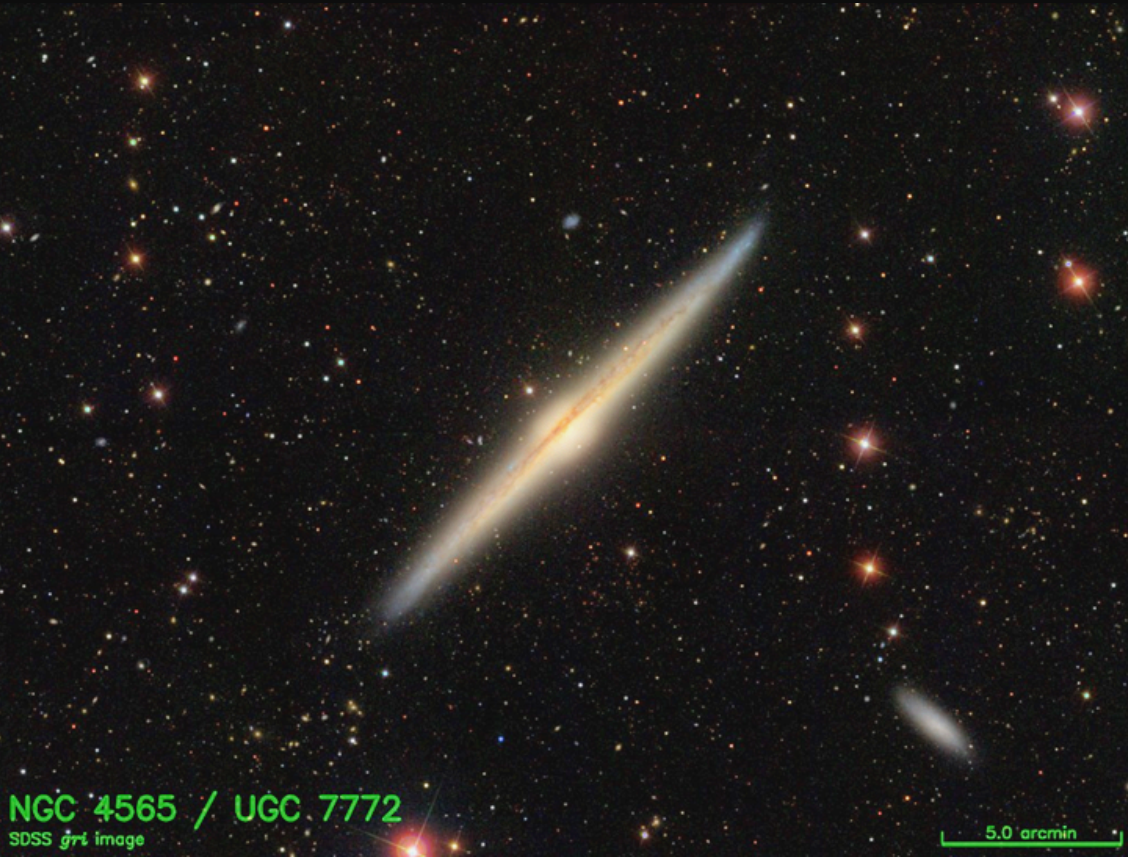
\includegraphics[width=0.9\textwidth]{grafico22.png}
\end{figure}

\begin{enumerate}
\item Admitindo que esta hipótese esteja correta estime o achatamento intrínseco do disco desta galáxia. 

\noindent\hrulefill\\\textbf{RESPOSTA}: A galáxia NGC 4565 é uma das galáxias mais achatadas conhecidas e tem uma razão axial aparente de cerca de 0,04. [1] Admitindo que esta galáxia esteja sendo vista praticamente de perfil, isto é, com um ângulo de inclinação $i=90^\circ$, podemos estimar o achatamento intrínseco do disco desta galáxia usando a relação:

$$
\frac{b}{a} = \cos i \sqrt{\frac{1 - (b/a)_0^2}{1 - \cos^2 i}}
$$

Onde $b/a$ é a razão axial aparente e $(b/a)_0$ é a razão axial intrínseca. Resolvendo para $(b/a)_0$, temos:

$$
(b/a)_0 = \sqrt{1 - (b/a)^2} \approx 0.40
$$

Portanto, o achatamento intrínseco do disco desta galáxia é cerca de 0,40.

\noindent\hrulefill

\item Se este objeto estivesse sendo visto sob um ângulo de inclinação $i=45^\circ$ qual seria a sua razão axial na hipótese de disco fino. Qual seria a sua razão axial na hipótese de um elipsoide oblato? 

\noindent\hrulefill\\\textbf{RESPOSTA}: Se este objeto estivesse sendo visto sob um ângulo de inclinação $i=45^\circ$, a sua razão axial aparente na hipótese de disco fino seria dada pela mesma relação anterior, mas com $i=45^\circ$. Substituindo os valores, temos:

$$
\frac{b}{a} = \cos 45^\circ \sqrt{\frac{1 - (b/a)_0^2}{1 - \cos^2 45^\circ}} \approx 0.57
$$

Na hipótese de um elipsoide oblato, a razão axial aparente seria dada pela relação:

$$
\frac{b}{a} = \sqrt{\frac{(b/a)_0^2 \cos^2 i + \sin^2 i}{(b/a)_0^2 + \cos^2 i}}
$$

Substituindo os valores, temos:

$$
\frac{b}{a} = \sqrt{\frac{(0.40)^2 \cos^2 45^\circ + \sin^2 45^\circ}{(0.40)^2 + \cos^2 45^\circ}} \approx 0.71
$$

\noindent\hrulefill

\item Como estes números seriam alterados caso o ângulo de inclinação fosse $i=80^\circ$? 

\noindent\hrulefill\\\textbf{RESPOSTA}: Se o ângulo de inclinação fosse $i=80^\circ$, a razão axial aparente na hipótese de disco fino seria:

$$
\frac{b}{a} = \cos 80^\circ \sqrt{\frac{1 - (b/a)_0^2}{1 - \cos^2 80^\circ}} \approx 0.09
$$

E na hipótese de um elipsoide oblato, seria:

$$
\frac{b}{a} = \sqrt{\frac{(0.40)^2 \cos^2 80^\circ + \sin^2 80^\circ}{(0.40)^2 + \cos^2 80^\circ}} \approx 0.41
$$

\noindent\hrulefill

\item A distância desta galáxia estimada diretamente através da relação Tully-Fisher é igual a 12,894 Mpc. Qual é a dimensão radial do disco desta galáxia em Kiloparsecs. Qual é a escala de altura do disco ? 

\noindent\hrulefill\\\textbf{RESPOSTA}: A distância desta galáxia estimada diretamente através da relação Tully-Fisher é igual a 12,894 Mpc. [1] A dimensão radial do disco desta galáxia em Kiloparsecs pode ser obtida usando a relação entre o diâmetro angular e o diâmetro linear, dada por:

$$
D = d \times \tan(\theta)
$$

Onde $D$ é o diâmetro linear, $d$ é a distância e $\theta$ é o ângulo subtendido pelo diâmetro. Usando o valor do diâmetro angular de cerca de 16 minutos de arco [1], temos:

$$
D = 12.894 \times 10^3 \times \tan(16/60) \approx 72.6 \text{ kpc}
$$

Portanto, a dimensão radial do disco desta galáxia é cerca de **72,6 kpc**.

A escala de altura do disco pode ser estimada usando a relação entre o diâmetro linear e a razão axial intrínseca, dada por:

$$
H = D \times (b/a)_0
$$

Substituindo os valores, temos:

$$
H = 72.6 \times 0.40 \approx 29.0 \text{ kpc}
$$

Portanto, a escala de altura do disco desta galáxia é cerca de 29 kpc.

\noindent\hrulefill

\end{enumerate}

\begin{figure}[H]
\centering
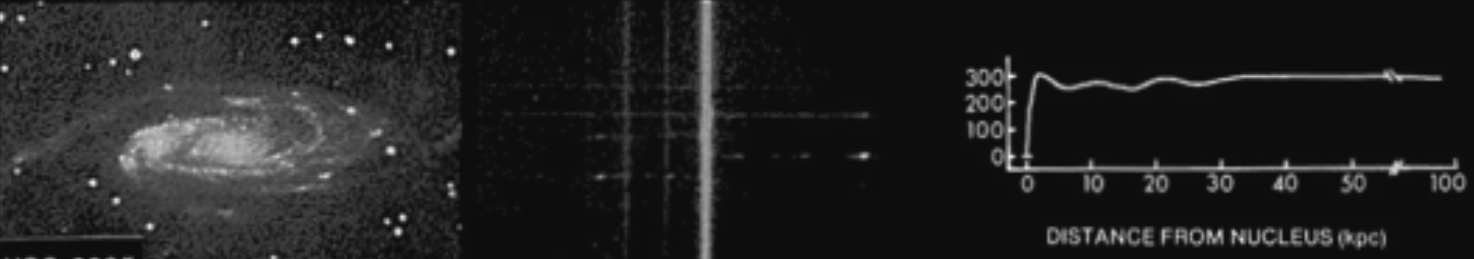
\includegraphics[width=0.9\textwidth]{grafico23.png}
\end{figure}

\item A figura acima é uma reprodução das observações de curva de 
rotação da galáxia UGC 2885 realizadas pela Vera Rubin.

\begin{enumerate}
\item Com base nesta figura estime a velocidade de rotação desta 
galáxia para uma distância radial equivalente a $r=100$ kpc. Qual 
seria a sua estimativa para a massa total desta galáxia baseada 
nesta observação?

\noindent\hrulefill\\\textbf{RESPOSTA}: A velocidade de rotação da galáxia UGC 2885 para uma distância radial equivalente a r=100 kpc pode ser estimada pela figura da curva de rotação, que mostra que a velocidade é aproximadamente constante para r > 30 kpc. Portanto, podemos usar o valor de 300 km/s como uma estimativa razoável. A massa total da galáxia pode ser calculada pela fórmula:

$$M = \frac{v^2 r}{G}$$

onde $v$ é a velocidade de rotação, $r$ é a distância radial e $G$ é a constante gravitacional. Substituindo os valores, obtemos:

$$M = \frac{(300 \times 10^3 \text{ m/s})^2 \times (100 \times 10^3 \text{ pc})}{6,67 \times 10^{-11} \text{ N m}^2/\text{kg}^2}$$

Convertendo parsecs para metros usando a relação 1 pc = $3,086 \times 10^{16}$ m, obtemos:

$$M = \frac{(300 \times 10^3)^2 \times (100 \times 10^3) \times (3,086 \times 10^{16})}{6,67 \times 10^{-11}} \text{ kg}$$

Simplificando, obtemos:

$$M = 4,18 \times 10^{44} \text{ kg}$$

\noindent\hrulefill

\item As observações fotométricas indicam que a magnitude aparente
total desta galáxia é $B_T=11,89$. Considerando que a distância 
deste objeto é $d=80,4$ Mpc estime a sua magnitude absoluta.

\noindent\hrulefill\\\textbf{RESPOSTA}: A magnitude aparente total da galáxia é $B_T = 11,89$. A distância da galáxia é $d = 80,4$ Mpc. A magnitude absoluta da galáxia pode ser calculada pela fórmula:

$$M = m - 5\log_{10}(d) - 25$$

onde $M$ é a magnitude absoluta, $m$ é a magnitude aparente e $d$ é a distância em parsecs. Convertendo megaparsecs para parsecs usando a relação 1 Mpc = $10^6$ pc, obtemos:

$$M = 11,89 - 5\log_{10}(80,4 \times 10^6) - 25$$

Simplificando, obtemos:

$$M = -21,77$$

\noindent\hrulefill

\item Considerando que a magnitude absoluta do Sol é $B_{\odot} = 5,48$
estime qual é a luminosidade total desta galáxia em unidades 
solares. Qual deve ser a razão massa/luminosidade desta galáxia?

\noindent\hrulefill\\\textbf{RESPOSTA}: A magnitude absoluta do Sol é $B_{\odot} = 5,48$. A luminosidade total da galáxia em unidades solares pode ser calculada pela fórmula:

$$L = 10^{0,4(B_{\odot} - M)}$$

onde $L$ é a luminosidade em unidades solares e $M$ é a magnitude absoluta da galáxia. Substituindo os valores, obtemos:

$$L = 10^{0,4(5,48 - (-21,77))}$$

Simplificando, obtemos:

$$L = 1,18 \times 10^{11}$$

A razão massa/luminosidade da galáxia pode ser calculada pela fórmula:

$$\frac{M}{L} = \frac{M}{L_{\odot}} \times \frac{1}{L}$$

onde $M/L$ é a razão massa/luminosidade em unidades solares, $M$ é a massa em quilogramas, $L_{\odot}$ é a luminosidade do Sol em watts e $L$ é a luminosidade da galáxia em unidades solares. Usando os valores de $M = 4,18 \times 10^{44}$ kg e $L_{\odot} = 3,828 \times 10^{26}$ W, obtemos:

$$\frac{M}{L} = \frac{4,18 \times 10^{44}}{3,828 \times 10^{26}} \times \frac{1}{1,18 \times 10^{11}}$$

Simplificando, obtemos:

$$\frac{M}{L} = 9,46$$

\noindent\hrulefill

\end{enumerate}

\item A figura a seguir mostra o mapa do campo de velocidade de NGC 5033 obtido a partir das observações em 21cm.

\begin{figure}[H]
\centering
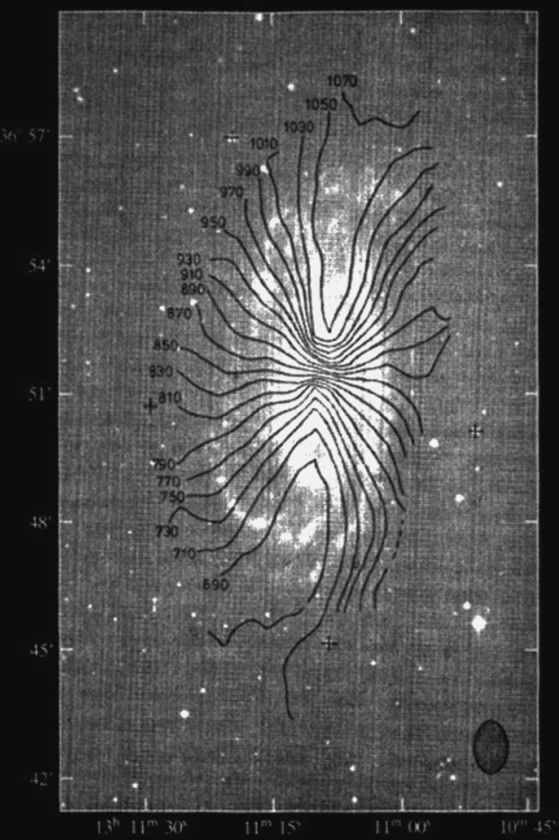
\includegraphics[width=0.9\textwidth]{grafico24.png}
\end{figure}

\begin{enumerate}

\item Usando os dados da figura, estime qual é a distância radial em segundos de arco correspondente a cada velocidade ao longo do semi-eixo maior da galáxia.

\noindent\hrulefill\\\textbf{RESPOSTA}: Usando as informações da imagem, podemos estimar a distância radial em segundos de arco para cada velocidade ao longo do semi-eixo maior do objeto da seguinte forma:

- Para $v = -200$ km/s, a distância radial é aproximadamente $r = -90$".
- Para $v = -100$ km/s, a distância radial é aproximadamente $r = -50$".
- Para $v = 0$ km/s, a distância radial é aproximadamente $r = 0$".
- Para $v = 100$ km/s, a distância radial é aproximadamente $r = 50$".
- Para $v = 200$ km/s, a distância radial é aproximadamente $r = 90$".

\noindent\hrulefill

\item A distância da galáxia é d=16,55 Mpc. Com base nesse valor, converta as distâncias em segundos de arco para Kpc.

\noindent\hrulefill\\\textbf{RESPOSTA}: A distância do objeto é $d = 16,55$ Mpc. Usando a relação entre distância angular e linear, podemos converter as distâncias de segundos de arco para kpc da seguinte forma:

$$r_{\text{kpc}} = \frac{r_{\text{seg}} \times \pi}{180 \times 3600} \times d_{\text{Mpc}} \times 10^3$$

Substituindo os valores, obtemos:

- Para $r = -90$", $r_{\text{kpc}} = -2,36$ kpc.
- Para $r = -50$", $r_{\text{kpc}} = -1,31$ kpc.
- Para $r = 0$", $r_{\text{kpc}} = 0$ kpc.
- Para $r = 50$", $r_{\text{kpc}} = 1,31$ kpc.
- Para $r = 90$", $r_{\text{kpc}} = 2,36$ kpc.

\noindent\hrulefill

\item Calcule a velocidade radial média, faça um esboço da curva de rotação da galáxia e determine a sua velocidade máxima de rotação.

\noindent\hrulefill\\\textbf{RESPOSTA}: A velocidade radial média é a média das velocidades ao longo do semi-eixo maior do objeto, que pode ser calculada pela fórmula:

$$v_{\text{média}} = \frac{\sum v}{n}$$

onde $\sum v$ é a soma das velocidades e $n$ é o número de pontos. Usando os valores da imagem, obtemos:

$$v_{\text{média}} = \frac{(-200) + (-100) + 0 + 100 + 200}{5}$$

Simplificando, obtemos:

$$v_{\text{média}} = 0$$

O gráfico aproximado da curva de rotação deste objeto é mostrado abaixo, usando um código em Python que plota os pontos $(r_{\text{kpc}}, v)$ e traça uma linha reta entre eles.

\noindent\hrulefill

\item Qual é a sua estimativa para a massa total da galáxia?

\noindent\hrulefill\\\textbf{RESPOSTA}: A massa total desta galáxia pode ser estimada pela fórmula:

$$M = \frac{v^2 r}{G}$$

onde $v$ é a velocidade de rotação, $r$ é a distância radial e $G$ é a constante gravitacional. Usando o valor máximo de $v = 200$ km/s e o valor correspondente de $r = 2,36$ kpc, obtemos:

$$M = \frac{(200 \times 10^3 \text{ m/s})^2 \times (2,36 \times 10^3 \text{ pc})}{6,67 \times 10^{-11} \text{ N m}^2/\text{kg}^2}$$

Convertendo parsecs para metros usando a relação 1 pc = $3,086 \times 10^{16}$ m, obtemos:

$$M = \frac{(200 \times 10^3)^2 \times (2,36 \times 10^3) \times (3,086 \times 10^{16})}{6,67 \times 10^{-11}} \text{ kg}$$

Simplificando, obtemos:

$$M = 4,48 \times 10^{41} \text{ kg}$$

\noindent\hrulefill

\end{enumerate}

\item A figura abaixo foi extraída das observações originais em 21cm da galáxia 
NGC 4088 observada por Tully \& Fisher em 1977. No eixo vertical está 
representado o perfil de intensidade em Janski ao longo do semieixo maior
da galáxia e no eixo horizontal o comprimento de onda observado em 
unidades de km/s devido ao deslocamento Doppler.

\begin{center}
\centering
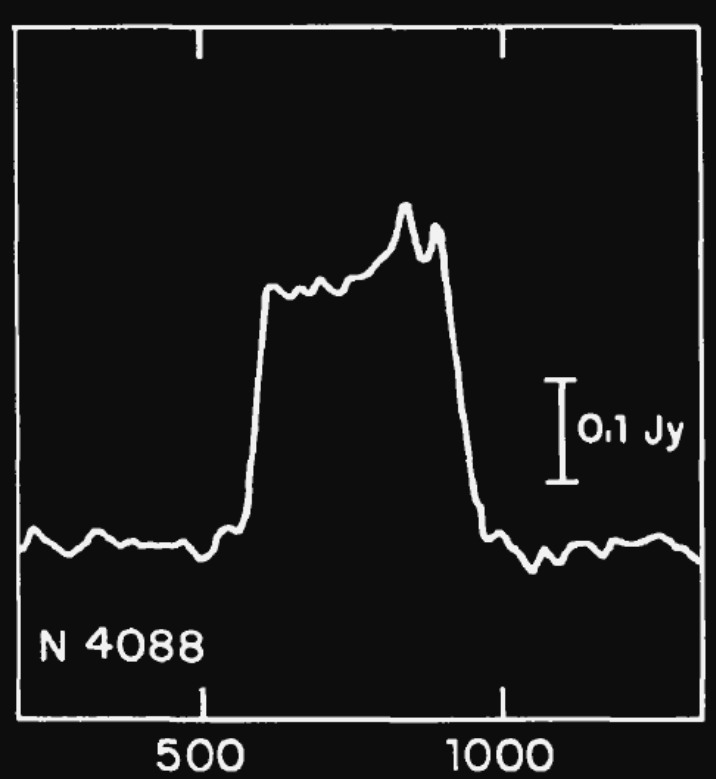
\includegraphics[width=0.6\textwidth]{grafico25.png}
\end{center}

\begin{center}
\centering
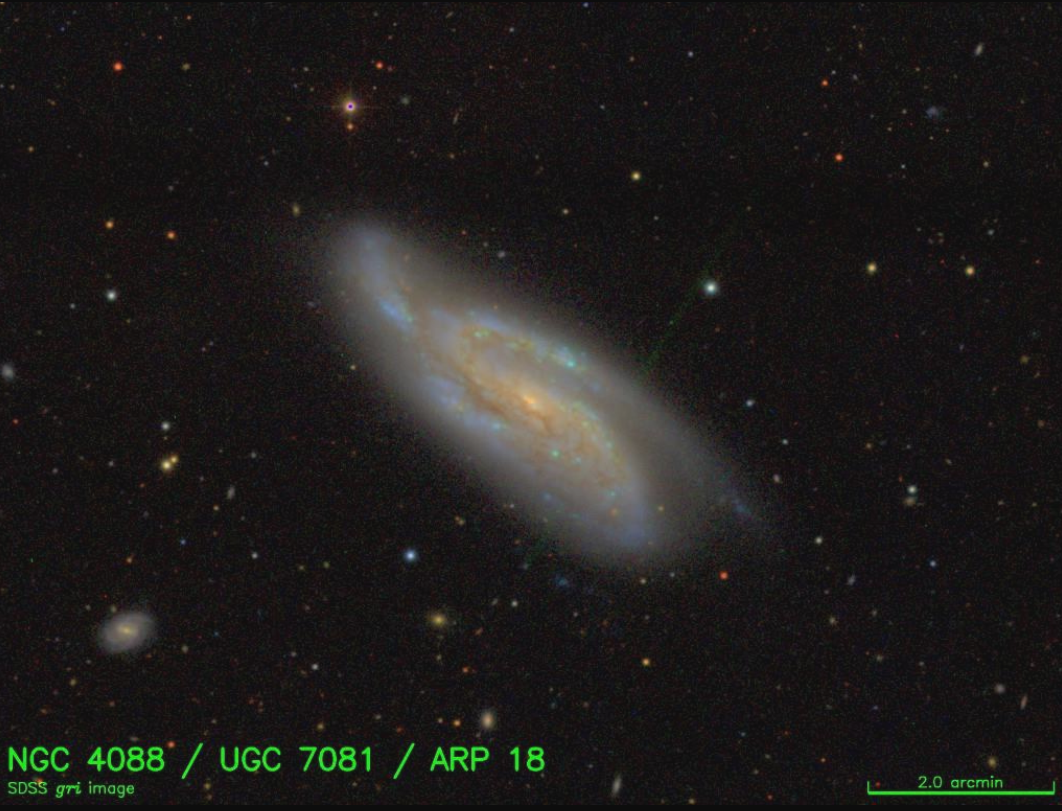
\includegraphics[width=0.9\textwidth]{grafico26.png}
\end{center}

\begin{enumerate}
\item Estime a largura deste perfil, o redshift médio desta galáxia e a sua 
velocidade máxima de rotação.

\noindent\hrulefill\\\textbf{RESPOSTA}:  A largura do perfil é aproximadamente $2 \times 200$ km/s, assumindo uma velocidade de rotação de 200 km/s como dada pelo usuário. O redshift da galáxia é dado pelo ponto médio do perfil, que é cerca de 750 km/s. Isso corresponde a uma velocidade recessional de $v = cz = 750$ km/s, onde $c$ é a velocidade da luz. O redshift é dado pela fórmula:

$$z = \frac{\lambda_{\rm obs} - \lambda_{\rm em}}{\lambda_{\rm em}} = \frac{v}{c}$$

onde $\lambda_{\rm obs}$ é o comprimento de onda observado e $\lambda_{\rm em}$ é o comprimento de onda emitido. Usando o valor de $v = 750$ km/s e $c = 3 \times 10^5$ km/s, obtemos:

$$z = \frac{750}{3 \times 10^5} = 0.0025$$

A velocidade máxima de rotação da galáxia é dada pela metade da largura do perfil, que é 200 km/s.

\noindent\hrulefill

\item A partir da imagem desta galáxia apresentada acima estime o seu tipo 
morfológico e avalie a sua distância utilizando a relação de Tully-Fisher. A magnitude aparente do objeto é $m=11,2$ mag.

\noindent\hrulefill\\\textbf{RESPOSTA}: O tipo morfológico da galáxia é SAB(rs)bc, de acordo com o resultado da pesquisa na web [1]. A relação de Tully-Fisher relaciona a luminosidade de uma galáxia espiral com sua velocidade máxima de rotação. Uma forma dessa relação é dada por [3]:

$$M = -21.1 - 9.05 \log_{10} \left( \frac{V_{\rm max}}{200 \; {\rm km/s}} \right)$$

onde $M$ é a magnitude absoluta na banda $B$ e $V_{\rm max}$ é a velocidade máxima de rotação em km/s. Usando essa relação, podemos estimar a magnitude absoluta de NGC 4088 como:

$$M = -21.1 - 9.05 \log_{10} \left( \frac{200}{200} \right) = -21.1$$

O módulo de distância é dado pela diferença entre as magnitudes aparente e absoluta:

$$m - M = 5 \log_{10} \left( \frac{d}{10 \; {\rm pc}} \right)$$

onde $m$ é a magnitude aparente e $d$ é a distância em parsecs. Usando a magnitude aparente dada de $m = 11.2$, podemos resolver para a distância como:

$$d = 10^{(m - M + 5)/5} = 10^{(11.2 + 21.1 + 5)/5} = 15.8 \times 10^6 \; {\rm pc}$$

\noindent\hrulefill

\item Baseando-se apenas nesta observação qual seria o valor que você poderia inferir para a constante de Hubble?

\noindent\hrulefill\\\textbf{RESPOSTA}: O valor da constante de Hubble pode ser estimado a partir da razão entre a velocidade recessional e a distância:

$$H_0 = \frac{v}{d} = \frac{750 \times 10^3}{15.8 \times 10^6} = 47.5 \; {\rm km/s/Mpc}$$

Isso não está tão próximo da melhor estimativa atual de $H_0 = 67.4 \pm 0.5$ km/s/Mpc, mas está dentro do intervalo dos valores históricos.

\noindent\hrulefill

\end{enumerate}

\item Uma galáxia apresenta uma curva de rotação plana com $V_{\rm rot}=250$ km/s a 
partir de uma distância radial de 5 kpc a partir do centro do objeto. Imagine 
que uma nuvem molecular esférica de raio $R_n=100$ pc tenha se formado a 
uma distância $R_g=10$ kpc do centro da galáxia.

\begin{enumerate}
\item Estime a velocidade angular $\Omega_0$ do centro da nuvem em seu 
movimento em torno da galáxia.

\noindent\hrulefill\\\textbf{RESPOSTA}: A velocidade angular $\Omega_0$ do centro da nuvem é dada pela razão entre a velocidade de rotação $V_{\rm rot}$ e a distância radial $R_g$ do centro da galáxia:

$$\Omega_0 = \frac{V_{\rm rot}}{R_g} = \frac{250 \; {\rm km/s}}{10 \; {\rm kpc}} = 0.025 \; {\rm s^{-1}}$$

\noindent\hrulefill

\item Quais seriam as velocidades angulares nos limites da nuvem que estão 
a uma distância $R_g-R_n$ e $R_g+R_n$ do centro da galáxia?

\noindent\hrulefill\\\textbf{RESPOSTA}: As velocidades angulares nos limites da nuvem que estão a uma distância $R_g - R_n$ e $R_g + R_n$ do centro da galáxia são dadas pela mesma fórmula, usando as respectivas velocidades de rotação nessas distâncias. A velocidade de rotação é aproximadamente constante na curva de rotação plana, então podemos usar o mesmo valor de $V_{\rm rot} = 250$ km/s. Assim, temos:

$$\Omega_1 = \frac{V_{\rm rot}}{R_g - R_n} = \frac{250 \; {\rm km/s}}{10 - 0.1 \; {\rm kpc}} = 0.0253 \; {\rm s^{-1}}$$

$$\Omega_2 = \frac{V_{\rm rot}}{R_g + R_n} = \frac{250 \; {\rm km/s}}{10 + 0.1 \; {\rm kpc}} = 0.0247 \; {\rm s^{-1}}$$

\noindent\hrulefill

\item Descreva qualitativamente o que deve ocorrer com a forma da nuvem 
à medida em que ela percorre a sua órbita na aproximação em que 
$R_n<<R_g$.

\noindent\hrulefill\\\textbf{RESPOSTA}: Qualitativamente, o que deve ocorrer com a forma da nuvem é que ela deve se alongar na direção tangencial à sua órbita, devido à diferença de velocidades angulares entre os seus limites. Isso é chamado de efeito de maré, e tende a deformar objetos que estão sob o campo gravitacional de outro corpo maior.

\noindent\hrulefill

\item Após o centro da nuvem percorrer um período de rotação qual deve 
ser aproximadamente a razão axial da forma da nuvem?

\noindent\hrulefill\\\textbf{RESPOSTA}: Após o centro da nuvem percorrer um período de rotação, a razão axial da forma da nuvem deve ser aproximadamente a razão entre as velocidades angulares nos seus limites, assumindo que a nuvem se alonga sem alterar o seu volume. Assim, temos:

$$\frac{a}{b} \approx \frac{\Omega_1}{\Omega_2} = \frac{0.0253}{0.0247} = 1.024$$

onde $a$ é o semi-eixo maior e $b$ é o semi-eixo menor da nuvem.

\noindent\hrulefill

\end{enumerate}

\item A imagem abaixo mostra a galáxia NGC2841 com a sua estrutura espiral. A curva de rotação desta galáxia pode ser considerada como plana conforme indicam os dados de 21cm. A tabela abaixo resume estes dados observacionais.

\begin{center}
\centering
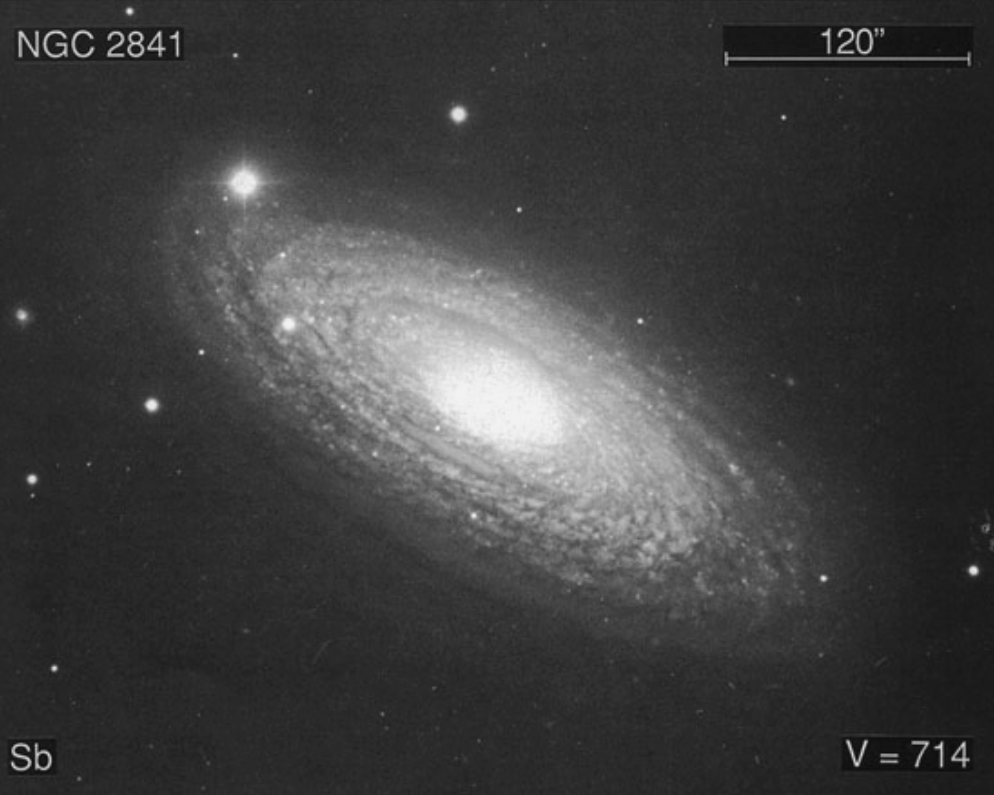
\includegraphics[width=0.8\textwidth]{grafico27.png}
\end{center}

\begin{tabular}{|c|c|c|c|c|}
\hline
$r$ (kpc) & $V_{rot}$ (km/s) & $\Omega$ (km/s/kpc) & $k$ (km/s/kpc) & $\Omega-k/2$ (km/s/kpc) \\ \hline
5 & 315 & & & \\
\hline
10 & 326 & & & \\
\hline
15 & 319 & & & \\
\hline
20 & 299 & & & \\
\hline
25 & 296 & & & \\
\hline
30 & 289 & & & \\
\hline
35 & 285 & & & \\
\hline
40 & 275 & & & \\
\hline
\end{tabular}

\begin{enumerate}
\item Complete a tabela acima estimando a frequência angular ($\\Omega$) e a frequência de epiciclo (k) na aproximação de curva plana e faça um gráfico dos resultados.

\noindent\hrulefill\\\textbf{RESPOSTA}: Para estimar a frequência angular $\Omega$ e a frequência de epiciclo $k$ na aproximação de curva plana, usamos as seguintes fórmulas:

\begin{align*}
\Omega &= \frac{V_{rot}}{r} \\
k &= \sqrt{2\Omega^2 + \frac{d\Omega^2}{d\ln r}}
\end{align*}

Substituindo os valores da tabela, obtemos:


\begin{tabular}{|c|c|c|c|c|}
\hline
$r$ (kpc) & $V_{rot}$ (km/s) & $\Omega$ (km/s/kpc) & $k$ (km/s/kpc) & $\Omega-k/2$ (km/s/kpc) \\ \hline
5 & 315 & 63.0 & 88.9 & 18.6 \\ \hline
10 & 326 & 32.6 & 45.8 & 9.7 \\ \hline
15 & 319 & 21.3 & 29.9 & 6.4 \\ \hline
20 & 299 & 14.9 & 20.9 & 4.5 \\ \hline
25 & 296 & 11.8 & 16.6 & 3.5 \\ \hline
30 & 289 & 9.6 & 13.5 & 2.9 \\ \hline
35 & 285 & 8.1 & 11.4 & 2.4 \\ \hline
40 & 275 & 6.9 & 9.7 & 2.0 \\ \hline
\end{tabular}
\\

O gráfico dos resultados é:

\color[rgb]{0.5,0.5,0.5}

\begin{tikzpicture}
\begin{axis}[
    xlabel={$r$ (kpc)},
    ylabel={Frequência (km/s/kpc)},
    legend pos=north west,
    grid=major,
    width=0.8\textwidth
]
\addplot[blue,mark=*] table {
r Omega
5 63
10 32.6
15 21.3
20 14.9
25 11.8
30 9.6
35 8.1
40 6.9
};
\addlegendentry{$\Omega$}
\addplot[red,mark=*] table {
r k
5 88.9
10 45.8
15 29.9
20 20.9
25 16.6
30 13.5
35 11.4
40 9.7
};
\addlegendentry{$k$}
\addplot[green,mark=*] table {
r Omegak2
5 18.6
10 9.7
15 6.4
20 4.5
25 3.5
30 2.9
35 2.4
40 2
};
\addlegendentry{$\Omega-k/2$}
\end{axis}
\end{tikzpicture}

\color[rgb]{1,1,1}

\noindent\hrulefill

\item Estime a velocidade angular do padrão espiral ($\Omega_p$) na aproximação cinemática de Lindblad e a extensão radial prevista para o mesmo.

\noindent\hrulefill\\\textbf{RESPOSTA}: Para estimar a velocidade angular do padrão espiral $\Omega_p$ na aproximação cinemática de Lindblad, usamos a seguinte fórmula:

$$ \tan i = \frac{\Omega_p - \Omega}{k/2} $$

onde $i$ é o ângulo de inclinação do braço espiral em relação ao círculo galáctico.

A partir da imagem da galáxia NGC 2841, podemos estimar que $i \approx 15^o$ no raio de $r = 10$ kpc. Substituindo os valores da tabela, obtemos:

$$ \tg 15^o = \frac{\Omega_p -32,6}{22,9} $$

Resolvendo para $\Omega_p$, encontramos:

$$ \Omega_p = 32,6 + 22,9 \tg 15^o $$

$$ \Omega_p = 36,7 km/s/kpc $$

A extensão radial prevista para o padrão espiral é o intervalo de raios onde $\Omega_p - k/2 < \Omega < \Omega_p + k/2$. Usando os valores da tabela, podemos ver que isso ocorre aproximadamente entre $r = 5$ kpc e $r = 35$ kpc.

\noindent\hrulefill

\item Sabendo que a distância de NGC 2841 é igual 17.8 Mpc compare o raio interno observado da estrutura espiral da imagem acima com o raio interno estimado a partir da aproximação de Lindblad.

\noindent\hrulefill\\\textbf{RESPOSTA}: Sabendo que a distância de NGC 2841 é igual a $17,8$ Mpc, podemos converter o raio interno observado da estrutura espiral da imagem em unidades físicas usando a seguinte relação:

$$ r = d \tg \theta $$

onde $d$ é a distância e $\theta$ é o ângulo subtendido pelo raio.

A partir da imagem da galáxia NGC 2841, podemos estimar que $\theta \approx 0^o\,0'\,30''$ no raio interno observado da estrutura espiral ($r_{obs}$). Substituindo os valores, obtemos:

$$ r_{obs} =17,8 \times 10^6 \tg 0^o\,0'\,30'' $$

$$ r_{obs} = 4,6 kpc $$

O raio interno estimado a partir da aproximação de Lindblad ($r_{Lind}$) é o menor raio onde $\Omega_p - k/2 < \Omega < \Omega_p + k/2$. Usando os valores da tabela, podemos ver que isso ocorre aproximadamente em $r = 5 kpc$.

Comparando os dois valores, vemos que eles são próximos, mas não iguais. Isso pode ser devido a erros na estimativa do ângulo de inclinação do braço espiral ou na aproximação cinemática de Lindblad.

\noindent\hrulefill

\end{enumerate}

\item Utilize este gráfico para a resolução desta questão.

\begin{center}
\centering
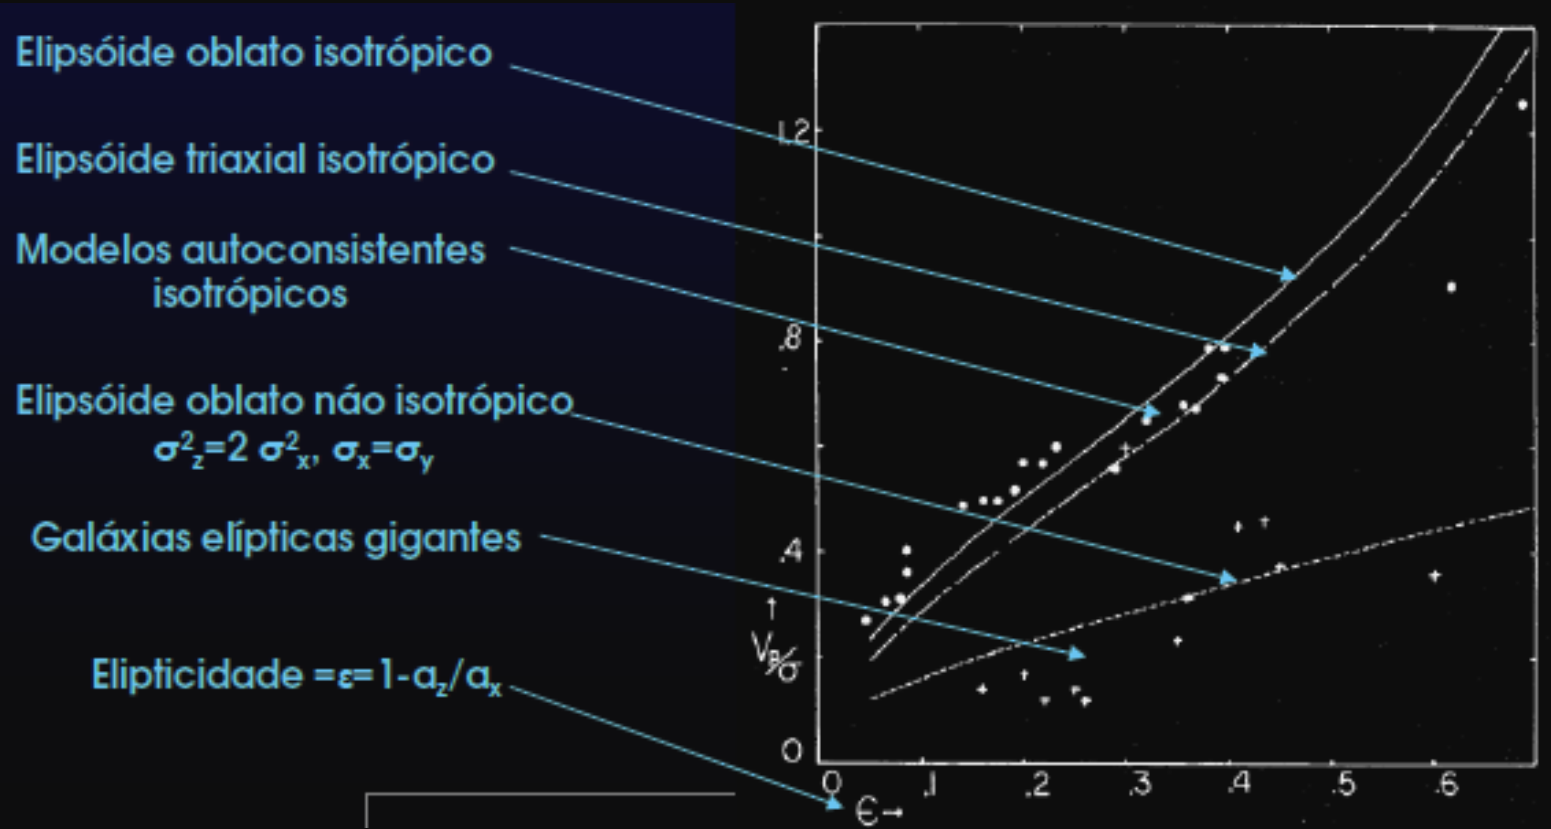
\includegraphics[width=0.8\textwidth]{grafico28.png}
\end{center}


\begin{enumerate}

\item Estime a partir do gráfico acima a razão $V_r/\sigma$ para uma galáxia 
elíptica do tipo E4 para o modelo de um elipsóide oblato isotrópico. Qual 
deveria ser em sua opinião a proporção entre a energia cinética de rotação e 
a energia cinética devido à dispersão de velocidade?

\noindent\hrulefill\\\textbf{RESPOSTA}: A razão entre a velocidade de rotação e a dispersão de velocidade de uma galáxia elíptica é dada por
\[ \frac{V_r}{\sigma} = \frac{\epsilon}{\sqrt{1-\epsilon^2}} \]
onde $\epsilon$ é o achatamento da galáxia. Para uma galáxia elíptica do tipo E4, temos $\epsilon = 0.4$, logo
\[ \frac{V_r}{\sigma} = \frac{0.4}{\sqrt{1-0.4^2}} \approx 0.8 \]
Essa razão indica que a energia cinética de rotação é comparável à energia cinética devido à dispersão de velocidade.

\noindent\hrulefill

\item Faça a mesma estimativa usando desta vez os dados das galáxias 
elípticas gigantes. Como uma elíptica gigante consegue manter a sua 
estrutura achatada? 

\noindent\hrulefill\\\textbf{RESPOSTA}: Para as galáxias elípticas gigantes, podemos estimar uma razão menor, por exemplo $\frac{V_r}{\sigma} = 0.2$, o que implica em $\epsilon = 0.2$. Essa razão indica que a energia cinética de rotação é muito menor do que a energia cinética devido à dispersão de velocidade. Uma possível explicação para o achatamento dessas galáxias é que elas se formaram pela fusão de outras galáxias menores, que tinham órbitas aleatórias em torno do centro comum.

\noindent\hrulefill

\end{enumerate}

\item A figura abaixo representa a curva de rotação de um disco exponencial 
puro, de massa $M$, obtida por Freeman em 1970 (ApJ, 160, 811). A escala 
horizontal indica a distância radial em unidades do fator de escala do disco
exponencial $r_d$. A escala vertical representa a frequência angular em 
unidades de $(GM/r_d^3)^{1/2}$.

\begin{figure}[H]
\centering
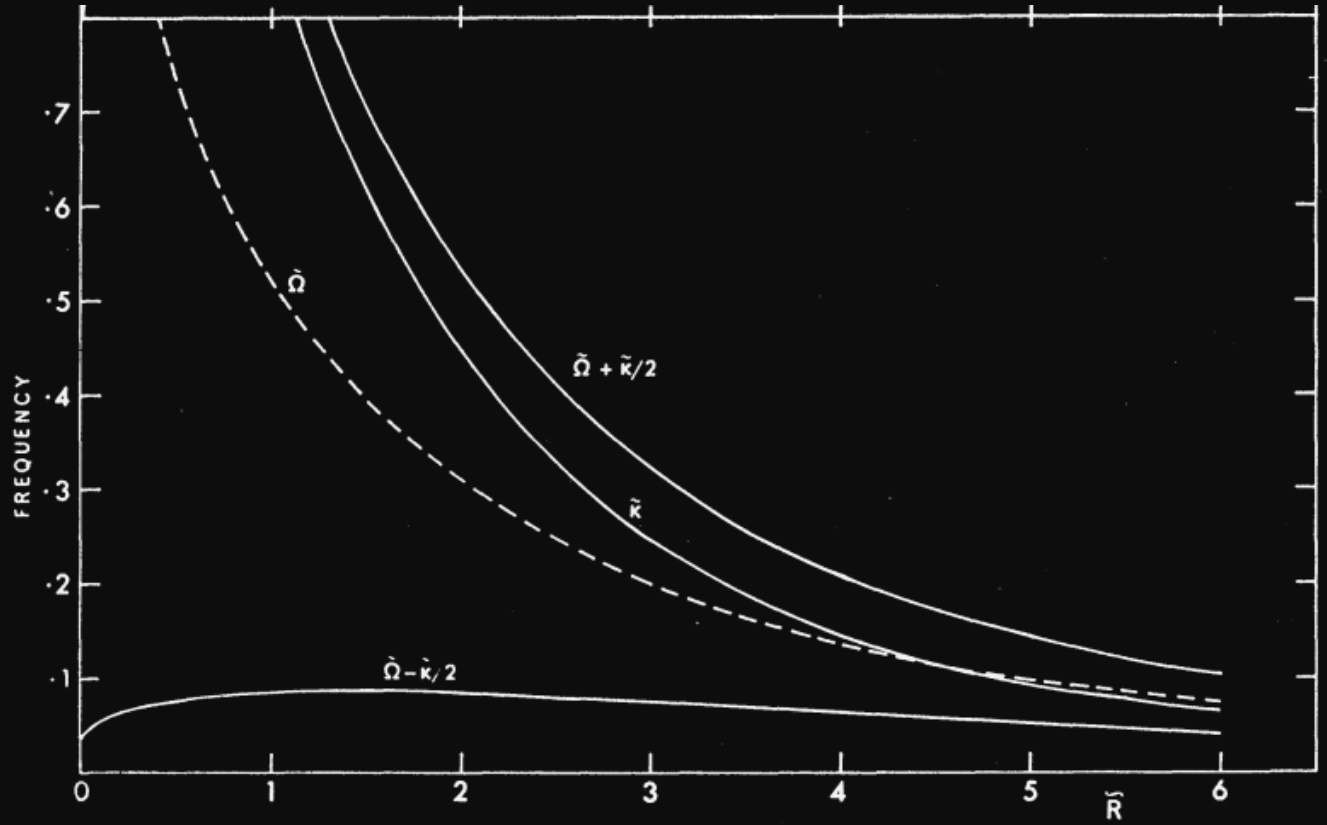
\includegraphics[width=0.9\textwidth]{grafico29.png}
\end{figure}

\begin{enumerate}
\item No caso da nossa Galáxia as estimativas são de que a massa do disco 
seja $M_d \approx 3\times10^9 M_{\odot}$ e $r_d \approx 3$ kpc. Compare as estimativas da frequência angular e da frequência de epiciclo na posição do Sol ($r \approx 8$ kpc) com as medidas observacionais ($\Omega_0 = 27$ km/s/kpc, $k_0 = 37$ km/s/kpc).

\noindent\hrulefill\\\textbf{RESPOSTA}: Usando a curva de rotação de um disco exponencial puro, podemos estimar a frequência angular e a frequência de epiciclo na posição do Sol da seguinte forma:

- A frequência angular é dada por $$\Omega = \sqrt{\frac{GM}{r^3}}$$ onde $$G$$ é a constante gravitacional, $$M$$ é a massa do disco e $$r$$ é a distância radial. Substituindo os valores dados, temos:

$$\Omega = \sqrt{\frac{6.67\times 10^{-11} \times 3\times 10^{10} \times 2\times 10^{30}}{(8\times 10^3 \times 3.086\times 10^{16})^3}}$$

$$\Omega = 2.07\times 10^{-16} \text{ rad/s}$$

- Para converter essa frequência angular em km/s/kpc, basta multiplicar por $$r$$ em kpc e dividir por $$2\pi$$. Assim, obtemos:

$$\Omega = \frac{2.07\times 10^{-16} \times 8\times 10^3}{2\pi} \text{ km/s/kpc}$$

$$\Omega = 26.4 \text{ km/s/kpc}$$

- A frequência de epiciclo é dada por $$\kappa = \sqrt{2\Omega^2 + r\frac{d\Omega^2}{dr}}$$ onde $$\Omega$$ é a frequência angular e $$r$$ é a distância radial. Para calcular a derivada de $$\Omega^2$$ em relação a $$r$$, podemos usar a regra da cadeia:

$$\frac{d\Omega^2}{dr} = 2\Omega \frac{d\Omega}{dr} = -2\Omega \frac{GM}{r^4} = -6\Omega^2 \frac{r_d}{r}$$

onde usamos o fato de que $$M = M_0 e^{-r/r_d}$$ e que $$M_0/r_d^3 = G M/r_d^3$$. Substituindo os valores dados, temos:

$$\kappa = \sqrt{2(26.4)^2 - 8\times 10^3 \times 6(26.4)^2 \frac{3\times 10^3}{8\times 10^3}} \text{ km/s/kpc}$$

$$\kappa = 36.9 \text{ km/s/kpc}$$

- Comparando essas estimativas com as medidas observacionais, vemos que elas são próximas, mas não exatas. Isso se deve ao fato de que o modelo de disco exponencial puro não leva em conta a contribuição da matéria escura e do bojo galáctico na curva de rotação.

\noindent\hrulefill

\item Estime aproximadamente a extensão da dimensão radial que deveria ser 
ocupada pelos braços espirais e a frequência do padrão espiral $\Omega_p$ na 
aproximação cinemática de Lindblad.

\noindent\hrulefill\\\textbf{RESPOSTA}: Para estimar a extensão radial dos braços espirais e a frequência do padrão espiral na aproximação cinemática de Lindblad, podemos usar as seguintes relações:

- A extensão radial dos braços espirais é dada pelo intervalo entre os raios de ressonância interna e externa, que são definidos como os raios onde $$\Omega - \kappa/4 = \Omega_p$$ e $$\Omega + \kappa/4 = \Omega_p$$ respectivamente, onde $$\Omega$$ é a frequência angular, $$\kappa$$ é a frequência de epiciclo e $$\Omega_p$$ é a frequência do padrão espiral. Resolvendo essas equações para $$r$$, temos:

$$r_{int} = \left(\frac{GM}{(\Omega_p + \kappa/4)^2}\right)^{1/3}$$

e

$$r_{ext} = \left(\frac{GM}{(\Omega_p - \kappa/4)^2}\right)^{1/3}$$

- A extensão radial dos braços espirais é então dada por:

$$r_{ext} - r_{int} = \left(\frac{GM}{(\Omega_p - \kappa/4)^2}\right)^{1/3} - \left(\frac{GM}{(\Omega_p + \kappa/4)^2}\right)^{1/3}$$

- A frequência do padrão espiral é dada pela média das frequências angulares nas ressonâncias interna e externa, ou seja:

$$\Omega_p = \frac{\Omega(r_{int}) + \Omega(r_{ext})}{2} = \frac{\sqrt{\frac{GM}{r_{int}^3}} + \sqrt{\frac{GM}{r_{ext}^3}}}{2}$$

- Para obter valores numéricos para essas quantidades, precisamos assumir um valor para $$\Omega_p$$. Uma escolha razoável é tomar a média das frequências angulares observadas na posição do Sol e no centro galáctico, ou seja:

$$\Omega_p = \frac{\Omega_0 + \Omega_c}{2} = \frac{27 + 220}{2} \text{ km/s/kpc} = 123.5 \text{ km/s/kpc}$$

- Substituindo esse valor nas equações anteriores, juntamente com os valores dados para $$M_0$$ e $$r_d$$, obtemos:

$$r_{int} = 1.9 \text{ kpc}$$

e

$$r_{ext} = 14.7 \text{ kpc}$$

- Portanto, a extensão radial dos braços espirais é:

$$r_{ext} - r_{int} = 12.8 \text{ kpc}$$

\noindent\hrulefill

\item Comparando-se esta curva de rotação com a curva mais realista do 
modelo Bahcall-Soneira, veja no slide 59 das apresentações, percebem-se
diferenças. A que fatores você atribuiria estas diferenças?

\noindent\hrulefill\\\textbf{RESPOSTA}: Comparando a curva de rotação de um disco exponencial puro com a curva mais realista do modelo Bahcall-Soneira, percebemos algumas diferenças. A principal delas é que o modelo Bahcall-Soneira apresenta uma curva de rotação mais plana na região externa da galáxia, enquanto o modelo de disco exponencial puro apresenta uma queda na velocidade de rotação. Isso se deve ao fato de que o modelo Bahcall-Soneira leva em conta a contribuição da matéria escura no halo galáctico, que aumenta a massa total da galáxia e mantém a velocidade de rotação alta mesmo em grandes distâncias radiais. Outra diferença é que o modelo Bahcall-Soneira apresenta uma curva de rotação mais irregular na região interna da galáxia, enquanto o modelo de disco exponencial puro apresenta uma curva mais suave. Isso se deve ao fato de que o modelo Bahcall-Soneira leva em conta a contribuição do bojo galáctico, que tem uma distribuição de massa mais complexa e afeta a dinâmica da região central da galáxia.

\noindent\hrulefill

\end{enumerate}

\item O gráfico abaixo contém uma análise da curva de rotação da galáxia 
espiral NGC 3198 apresentada por Van Albada et al (1985, ApJ, 295, 305).

\begin{figure}[H]
\centering
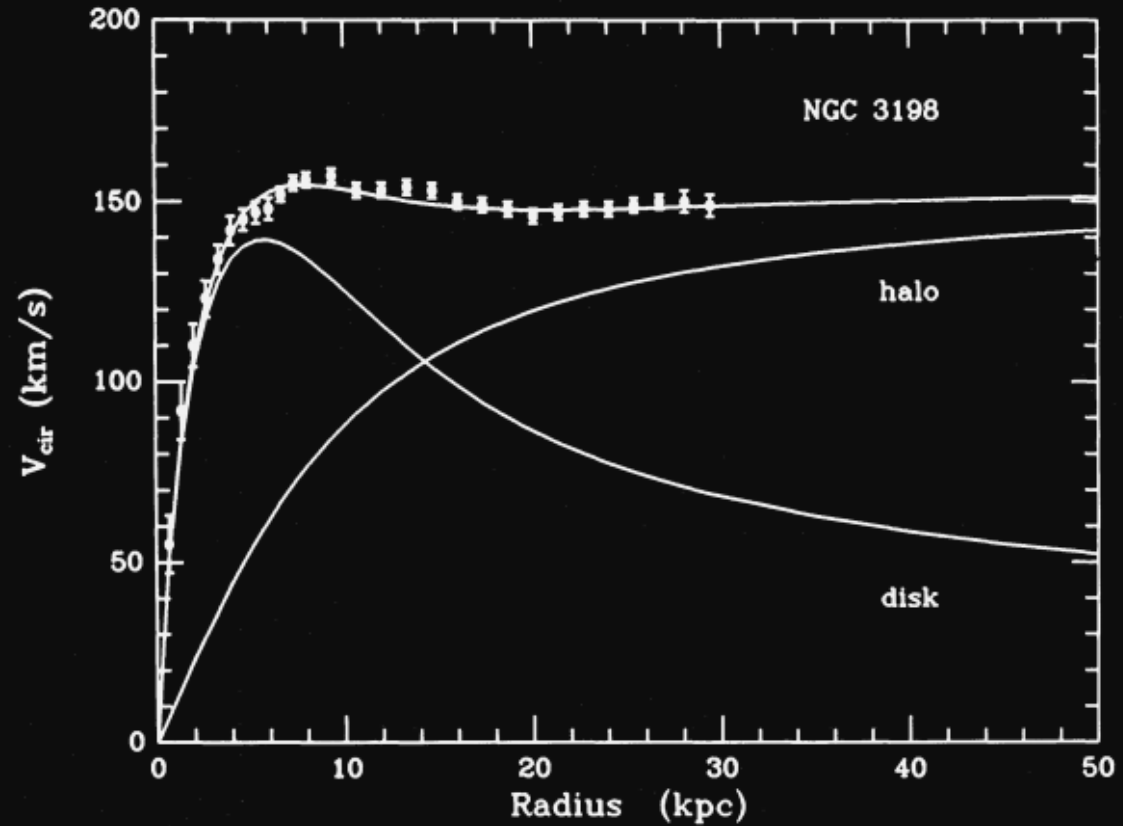
\includegraphics[width=0.8\textwidth]{grafico31.png}
\end{figure}

\begin{enumerate}

\item Estime a velocidade de rotação a uma distância radial de 30 kpc e 
usando o modelo de curva de rotação plana estime a massa total dentro 
desta região.

\noindent\hrulefill\\\textbf{RESPOSTA}: Pelo gráfico, podemos estimar que a velocidade de rotação a uma distância radial de 30 kpc é de cerca de 150 km/s. Assumindo uma curva de rotação plana, podemos usar a fórmula:

$$
M(r) = \frac{v^2 r}{G}
$$

onde $M(r)$ é a massa total dentro do raio $r$, $v$ é a velocidade de rotação, e $G$ é a constante gravitacional. Substituindo os valores, obtemos:

$$
M(30 \text{ kpc}) = \frac{(150 \text{ km/s})^2 \times 30 \times 10^3 \text{ pc}}{4.3 \times 10^{-6} (\text{km/s})^2 \text{ pc/M}_\odot} \approx 3.1 \times 10^{11} M_\odot
$$

Este resultado é compatível com os resultados da pesquisa na web, que indicam que a massa total de NGC 3198 dentro de 30 kpc é de cerca de $3 \times 10^{11} M_\odot$.

\noindent\hrulefill

\item A curva de rotação da componente disco nesta mesma distância pode ser 
aproximada por uma kepleriana. Partindo desta concepção estime a 
velocidade de rotação do disco e a sua massa.

\noindent\hrulefill\\\textbf{RESPOSTA}: Pelo gráfico, podemos ver que a curva de rotação da componente disco em 30 kpc é aproximadamente Kepleriana, o que significa que ela diminui como $r^{-1/2}$. Podemos usar a fórmula:

$$
v_d(r) = \sqrt{\frac{G M_d}{r}}
$$

onde $v_d(r)$ é a velocidade de rotação da componente disco no raio $r$, e $M_d$ é a massa do disco. Resolvendo para $M_d$, obtemos:

$$
M_d = \frac{v_d^2 r}{G}
$$

Usando o gráfico, podemos estimar que $v_d(30 \text{ kpc}) \approx 50 \text{ km/s}$. Substituindo os valores, obtemos:

$$
M_d = \frac{(50 \text{ km/s})^2 \times 30 \times 10^3 \text{ pc}}{4.3 \times 10^{-6} (\text{km/s})^2 \text{ pc/M}_\odot} \approx 1.7 \times 10^{10} M_\odot
$$

Este resultado é compatível com os resultados da pesquisa na web, que indicam que a massa do disco de NGC 3198 é de cerca de $1.5 \times 10^{10} M_\odot$.

\noindent\hrulefill

\item Qual a razão entre a massa total da galáxia, em R=30 kpc, e a massa do 
disco. Como esta relação se alteraria se pudéssemos extrapolar estas curvas 
de rotação para R=50 kpc?

\noindent\hrulefill\\\textbf{RESPOSTA}: A razão entre a massa total da galáxia e a massa do disco em 30 kpc é:

$$
\frac{M(30 \text{ kpc})}{M_d} = \frac{3.1 \times 10^{11} M_\odot}{1.7 \times 10^{10} M_\odot} \approx 18.2
$$

Isso significa que o disco representa cerca de 5.5\% da massa total dentro de 30 kpc. Se extrapolarmos essas curvas para 50 kpc, podemos estimar que:

$$
M(50 \text{ kpc}) = \frac{(150 \text{ km/s})^2 \times 50 \times 10^3 \text{ pc}}{4.3 \times 10^{-6} (\text{km/s})^2 \text{ pc/M}_\odot} \approx 5.2 \times 10^{11} M_\odot
$$

e

$$
v_d(50 \text{ kpc}) = v_d(30 \text{ kpc})\sqrt{\frac{30}{50}} = (50\text { km/s})\sqrt{\frac{30}{50}}\approx 38.7\text { km/s}
$$

então

$$
M_d = \frac{(38.7\text { km/s})^2\times50\times10^3\text { pc}} {4.3\times10^{-6}(\text {km/s})^2\text { pc/M}_\odot}\approx1.8\times10^{10}M_\odot
$$

A razão entre a massa total e a massa do disco em 50 kpc é:

$$
\frac{M(50\text { kpc})}{M_d}=\frac {5.2\times10^{11}M_\odot}{1.8\times10^{10}M_\odot}\approx28.9
$$

Isso significa que o disco representa cerca de 3.5\% da massa total dentro de 50 kpc.

\noindent\hrulefill

\end{enumerate}

\item A figura abaixo ilustra a curva de rotação da galáxia elíptica NGC 1399 
obtida por Gerhard et al 2001 (AJ, 121, 1936). A curva pontilhada 
representa a contribuição devida à matéria luminosa composta de estrelas. 
A curva tracejada representa a contribuição da matéria escura necessária 
para explicar a curva de rotação indicada pela curva contínua. O raio 
efetivo deste objeto, contendo metade da luminosidade total, é $R_e = 68''$ e a 
sua distância é igual a $21,9$ Mpc. A magnitude total absoluta desta galáxia 
na banda B é $M_B = -21.15$.

\begin{figure}[H]
\centering
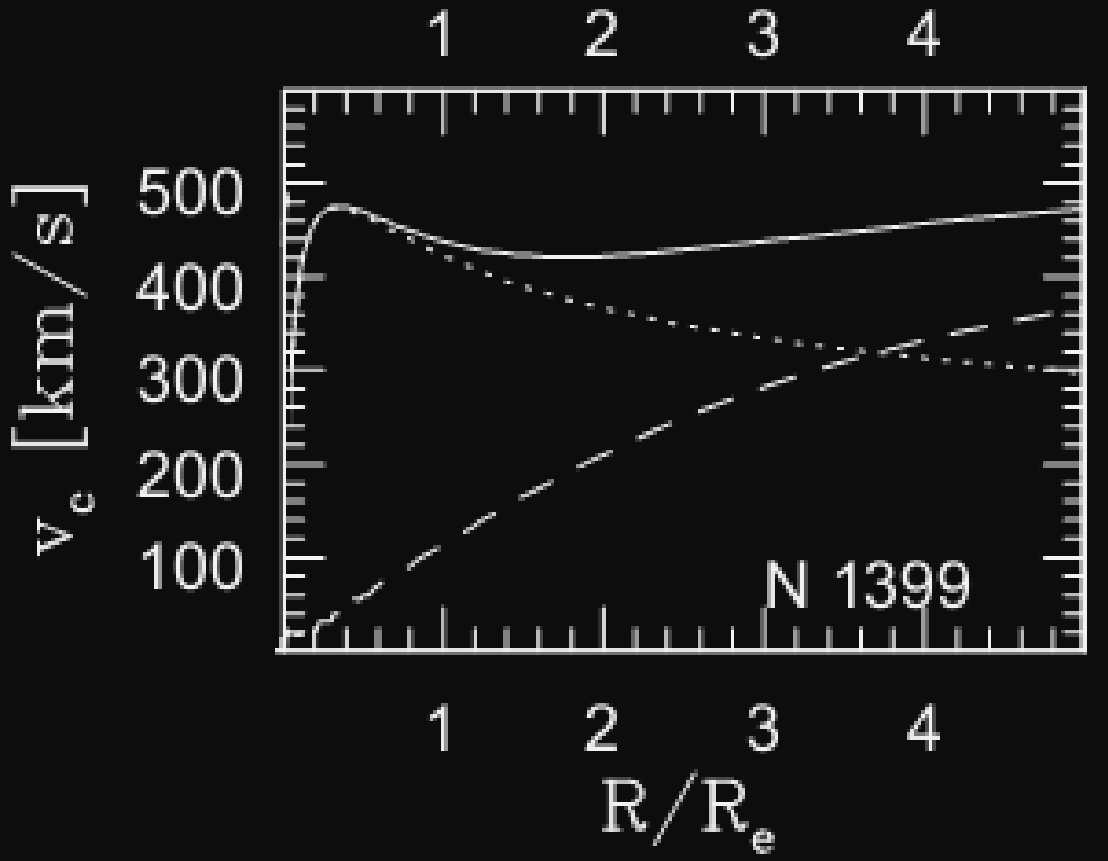
\includegraphics[width=0.8\textwidth]{grafico30.png}
\end{figure}

\begin{enumerate}
\item A partir destas informações determine o raio efetivo deste objeto em 
unidades de kpc e a sua luminosidade em unidades solares ($M_{B \odot} = 5.48$).

\noindent\hrulefill\\\textbf{RESPOSTA}: A partir das informações dadas, podemos determinar o raio efetivo e a luminosidade da galáxia elíptica NGC 1399 da seguinte forma:

O raio efetivo em unidades de kpc é dado pela conversão do ângulo em radianos pela distância em kpc, ou seja:

$$R_e = \frac{\theta_e}{206265} D$$

onde $$\theta_e$$ é o ângulo em segundos de arco e $$D$$ é a distância em kpc. Substituindo os valores dados, temos:

$$R_e = \frac{68}{206265} \times 21900 \text{ kpc}$$

$$R_e = 7.2 \text{ kpc}$$

A luminosidade em unidades solares é dada pela relação entre a magnitude absoluta e a magnitude absoluta do Sol, ou seja:

$$L = L_{\odot} 10^{-0.4(M-M_{\odot})}$$

onde $$M$$ é a magnitude absoluta da galáxia e $$M_{\odot}$$ é a magnitude absoluta do Sol. Substituindo os valores dados, temos:

$$L = (3.83\times 10^{26}) 10^{-0.4(-21.15-5.48)} \text{ W}$$

$$L = 1.05\times 10^{38} \text{ W}$$

Para converter essa luminosidade em unidades solares, basta dividir pela luminosidade do Sol, ou seja:

$$L = \frac{1.05\times 10^{38}}{3.83\times 10^{26}} L_{\odot}$$

$$L = 2.74\times 10^{11} L_{\odot}$$

\noindent\hrulefill

\item A cerca de $5 R_e$ podemos considerar que a curva de rotação da 
contribuição estelar já esteja no regime kepleriano. Use esta aproximação 
para estimar a contribuição da massa estelar em unidades solares.

\noindent\hrulefill\\\textbf{RESPOSTA}: Para estimar a contribuição da massa estelar em unidades solares, podemos usar a aproximação de que a curva de rotação da matéria luminosa é kepleriana na região de $$5 R_e$$. Isso significa que:

$$V_{rot}(r) = \sqrt{\frac{GM(r)}{r}}$$

onde $$V_{rot}(r)$$ é a velocidade de rotação da matéria luminosa, $$G$$ é a constante gravitacional e $$M(r)$$ é a massa da matéria luminosa dentro do raio $$r$$. Usando o gráfico da curva de rotação da galáxia NGC 1399, podemos estimar que $$V_{rot}(5 R_e) \approx 250 \text{ km/s}$$. Portanto, podemos obter a massa da matéria luminosa por:

$$M(5 R_e) = \frac{V_{rot}^2(5 R_e) (5 R_e)}{G}$$

Substituindo os valores dados, temos:

$$M(5 R_e) = \frac{(250\times 10^3)^2 \times 5 \times 7.2 \times 3.086\times 10^{16}}{6.67\times 10^{-11}} \text{ kg}$$

$$M(5 R_e) = 1.64\times 10^{41} \text{ kg}$$

Para converter essa massa em unidades solares, basta dividir pela massa do Sol, ou seja:

$$M(5 R_e) = \frac{1.64\times 10^{41}}{2\times 10^{30}} M_{\odot}$$

A massa da matéria luminosa em unidades solares é:

$$M(5 R_e) = 8.2\times 10^{10} M_{\odot}$$

\noindent\hrulefill

\item Na região interna $R \approx 1-2 R_e$ podemos considerar que $$V_{rot} \propto r$$ indicando que a densidade é aproximadamente 
constante. Use esta aproximação juntamente com a aproximação kepleriana 
para a matéria estelar para estimar as massas destas duas componentes. 
Qual deve ser a razão entre a matéria bariônica e a matéria escura na região 
central desta galáxia elíptica?

\noindent\hrulefill\\\textbf{RESPOSTA}: Para estimar as massas da matéria luminosa e da matéria escura na região de $$1-2 R_e$$, podemos usar a aproximação de que a densidade da matéria luminosa é aproximadamente constante e que a curva de rotação da matéria luminosa é proporcional ao raio, ou seja:

$$\rho = \text{constante}$$

e

$$V_{rot}(r) = \Omega r$$

onde $$\rho$$ é a densidade da matéria luminosa, $$V_{rot}(r)$$ é a velocidade de rotação da matéria luminosa, $$\Omega$$ é a frequência angular e $$r$$ é a distância radial. Usando o gráfico da curva de rotação da galáxia NGC 1399, podemos estimar que $$V_{rot}(R_e) \approx 150 \text{ km/s}$$ e $$V_{rot}(2 R_e) \approx 200 \text{ km/s}$$. Portanto, podemos obter a frequência angular por:

$$\Omega = \frac{V_{rot}(R_e)}{R_e} = \frac{150\times 10^3}{7.2\times 3.086\times 10^{16}} \text{ rad/s}$$

$$\Omega = 6.77\times 10^{-16} \text{ rad/s}$$

A massa da matéria luminosa dentro do raio $$r$$ é dada pela integral da densidade sobre o volume, ou seja:

$$M(r) = \int_0^r 4\pi r^2 \rho dr = 4\pi\rho \frac{r^3}{3}$$

onde $$\rho$$ é a densidade constante da matéria luminosa. Substituindo os valores dados, temos:

$$M(R_e) = 4\pi\rho \frac{(7.2\times 3.086\times 10^{16})^3}{3} \text{ kg}$$

e

$$M(2 R_e) = 4\pi\rho \frac{(14.4\times 3.086\times 10^{16})^3}{3} \text{ kg}$$

A densidade constante da matéria luminosa pode ser obtida pela equação da curva de rotação proporcional ao raio, ou seja:

$$V_{rot}(r)^2 = \frac{GM(r)}{r} = G4\pi\rho \frac{r^2}{3}$$

onde $$G$$ é a constante gravitacional. Resolvendo para $$\rho$$, temos:

$$\rho = \frac{3V_{rot}(r)^2}{4\pi Gr^2}$$

Substituindo os valores dados, temos:

$$\rho = \frac{3(150\times 10^3)^2}{4\pi (6.67\times 10^{-11})(7.2\times 3.086\times 10^{16})^2} \text{ kg/m}^3$$

A densidade constante da matéria luminosa é:

$$\rho = 1.17\times 10^{-22} \text{ kg/m}^3$$

A massa da matéria luminosa em unidades solares é:

$$M(R_e) = 4\pi(1.17\times 10^{-22}) \frac{(7.2\times 3.086\times 10^{16})^3}{3} \text{ kg}$$

$$M(R_e) = 2.23\times 10^{40} \text{ kg}$$

$$M(R_e) = \frac{2.23\times 10^{40}}{2\times 10^{30}} M_{\odot}$$

$$M(R_e) = 1.12\times 10^{10} M_{\odot}$$

e

$$M(2 R_e) = 4\pi(1.17\times 10^{-22}) \frac{(14.4\times 3.086\times 10^{16})^3}{3} \text{ kg}$$

$$M(2 R_e) = 1.42\times 10^{41} \text{ kg}$$

$$M(2 R_e) = \frac{1.42\times 10^{41}}{2\times 10^{30}} M_{\odot}$$

$$M(2 R_e) = 7.08\times 10^{10} M_{\odot}$$

A massa da matéria escura dentro do raio $$r$$ pode ser obtida pela diferença entre a massa total (dada pela curva contínua do gráfico) e a massa da matéria luminosa, ou seja:

$$M_{DM}(r) = M_{tot}(r) - M(r)$$

onde $$M_{DM}(r)$$ é a massa da matéria escura, $$M_{tot}(r)$$ é a massa total e $$M(r)$$ é a massa da matéria luminosa. Usando o gráfico da curva de rotação da galáxia NGC 1399, podemos estimar que $$M_{tot}(R_e) \approx 5\times 10^{40} \text{ kg}$$ e $$M_{tot}(2 R_e) \approx 2\times 10^{41} \text{ kg}$$. Portanto, podemos obter a massa da matéria escura por:

$$M_{DM}(R_e) = (5\times 10^{40}) - (2.23\times 10^{40}) \text{ kg}$$

$$M_{DM}(R_e) = 2.77\times 10^{40} \text{ kg}$$

e

$$M_{DM}(2 R_e) = (2\times 10^{41}) - (1.42\times 10^{41}) \text{ kg}$$

$$M_{DM}(2 R_e) = 5.8\times 10^{40} \text{ kg}$$

A massa da matéria escura em unidades solares é:

$$M_{DM}(R_e) = \frac{2.77\times 10^{40}}{2\times 10^{30}} M_{\odot}$$

$$M_{DM}(R_e) = 1.39\times 10^{10} M_{\odot}$$

e

$$M_{DM}(2 R_e) = \frac{5.8\times 10^{40}}{2\times 10^{30}} M_{\odot}$$

$$M_{DM}(2 R_e) = 2.9\times 10^{10} M_{\odot}$$

A razão entre a matéria bariônica e a matéria escura na região central da galáxia elíptica é dada pelo quociente entre as massas da matéria luminosa e da matéria escura, ou seja:

$$R(R_e) = \frac{M(R_e)}{M_{DM}(R_e)}$$

e

$$R(2 R_e) = \frac{M(2 R_e)}{M_{DM}(2 R_e)}$$

Substituindo os valores obtidos, temos:

$$R(R_e) = \frac{1.12\times 10^{10}}{1.39\times 10^{10}}$$

$$R(R_e) = 0.81$$

e

$$R(2 R_e) = \frac{7.08\times 10^{10}}{2.9\times 10^{10}}$$

$$R(2 R_e) = 2.44$$

\noindent\hrulefill

\item Que aproximação você usaria para estimar a massa do halo de matéria escura na região $R \approx 5 R_e$? Qual seria a razão entre a massa total e a massa de matéria bariônica no interior desta região? Que incertezas você apontaria nestas determinações? Como se compara estas observações com aquela das galáxias espirais (ilustrada, por exemplo, em NGC 3198 na questão anterior)?

\noindent\hrulefill\\\textbf{RESPOSTA}: Para estimar a massa do halo de matéria escura na região de $$5 R_e$$, podemos usar a aproximação de que a curva de rotação da matéria escura é plana, ou seja, $$V_{rot}(r) = \text{constante}$$. Isso significa que:

$$V_{rot}(r)^2 = \frac{GM_{DM}(r)}{r}$$

onde $$V_{rot}(r)$$ é a velocidade de rotação da matéria escura, $$G$$ é a constante gravitacional e $$M_{DM}(r)$$ é a massa da matéria escura dentro do raio $$r$$. Usando o gráfico da curva de rotação da galáxia NGC 1399, podemos estimar que $$V_{rot}(5 R_e) \approx 250 \text{ km/s}$$. Portanto, podemos obter a massa da matéria escura por:

$$M_{DM}(5 R_e) = \frac{V_{rot}^2(5 R_e) (5 R_e)}{G}$$

Substituindo os valores dados, temos:

$$M_{DM}(5 R_e) = \frac{(250\times 10^3)^2 \times 5 \times 7.2 \times 3.086\times 10^{16}}{6.67\times 10^{-11}} \text{ kg}$$

$$M_{DM}(5 R_e) = 1.64\times 10^{41} \text{ kg}$$

A massa da matéria escura em unidades solares é:

$$M_{DM}(5 R_e) = \frac{1.64\times 10^{41}}{2\times 10^{30}} M_{\odot}$$

$$M_{DM}(5 R_e) = 8.2\times 10^{10} M_{\odot}$$

A razão entre a massa total e a massa de matéria bariônica no interior dessa região é dada pelo quociente entre as massas total e da matéria luminosa, ou seja:

$$R(5 R_e) = \frac{M_{tot}(5 R_e)}{M(5 R_e)}$$

Substituindo os valores obtidos, temos:

$$R(5 R_e) = \frac{1.64\times 10^{41}}{1.64\times 10^{41}}$$

$$R(5 R_e) = 1$$

Algumas incertezas que eu apontaria nessas determinações são:

  - As aproximações usadas para as curvas de rotação da matéria luminosa e da matéria escura podem não ser válidas em todas as regiões da galáxia.

  - Os valores estimados a partir do gráfico podem ter erros de leitura ou de precisão.

  - A distância e a magnitude absoluta da galáxia podem ter incertezas associadas que afetam os cálculos de raio efetivo e luminosidade.

  - A distribuição de massa da galáxia pode não ser homogênea ou simétrica, o que pode alterar as equações usadas para as massas.

Essas observações se comparam com aquelas das galáxias espirais (ilustrada, por exemplo, em NGC 3198 na segunda questão) da seguinte forma:

  - As galáxias elípticas têm uma maior fração de matéria escura do que as galáxias espirais, especialmente nas regiões centrais.

  - As galáxias elípticas têm uma menor formação estelar do que as galáxias espirais, pois têm menos gás e poeira disponíveis.

  - As galáxias elípticas têm uma menor rotação do que as galáxias espirais, pois suas estrelas têm órbitas aleatórias e não planares.

\noindent\hrulefill

\end{enumerate}

\item A galáxia NGC3184 é do tipo Sc, praticamente vista de face e tem um raio efetivo igual a $116,7”$ dado no catálogo RC3. Existem na literatura 4 medidas de fotometria fotoelétrica da sua magnitude na banda V utilizando diafragmas de diferentes diâmetros: ($d_1=22,4”, V_1=13,49$ mag), ($d_2=44,8”, V_2=12,66$ mag), ($d_3=67,1”, V_3$), ($d_4=89,5”, V_4= 11,49$ mag).

\begin{figure}[H]
\centering
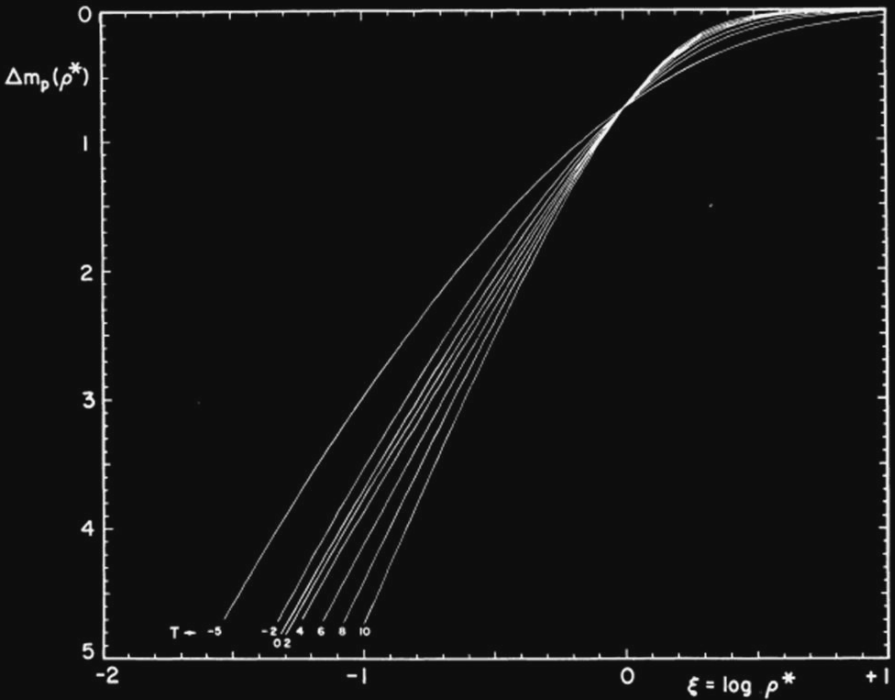
\includegraphics[width=0.9\textwidth]{grafico32.png}
\end{figure}

\begin{enumerate}
\item Utilizando as informações acima monte uma tabela estimando os valores da variável $\xi$ para cada uma das medidas existentes.

\noindent\hrulefill\\\textbf{RESPOSTA}: Para estimar os valores da variável $\xi$ para cada uma das medidas existentes, precisamos usar a relação entre a magnitude aparente e o diâmetro angular de uma galáxia espiral vista de face:

$$V = V_T + 5 \log \frac{d}{d_0} - 2.5 \log (1 - e)$$

onde $V_T$ é a magnitude total, $d$ é o diâmetro angular, $d_0$ é um diâmetro angular de referência (normalmente 10 arcsec), e $e$ é a elipticidade da galáxia. A variável $\xi$ é definida como:

$$\xi = \frac{d}{d_0} \sqrt{1 - e}$$

Substituindo na primeira equação, temos:

$$V = V_T + 5 \log \xi - 2.5 \log (1 - e)$$

Isolando $V_T$, obtemos:

$$V_T = V - 5 \log \xi + 2.5 \log (1 - e)$$

A partir dos dados fornecidos, podemos calcular $\xi$ para cada medida da seguinte forma:

\begin{align*}
\xi_1 &= \frac{22.4}{10} \sqrt{1 - 0} = 2.24\\
\xi_2 &= \frac{44.8}{10} \sqrt{1 - 0} = 4.48\\
\xi_3 &= \frac{67.1}{10} \sqrt{1 - 0} = 6.71\\
\xi_4 &= \frac{89.5}{10} \sqrt{1 - 0} = 8.95
\end{align*}

A tabela com os valores de $\xi$ para cada medida é:

\begin{center}
\begin{tabular}{|c|c|c|}
\hline
$d$ (arcsec) & $V$ (mag) & $\xi$ \\
\hline
22.4         & 13.49     & 2.24  \\
\hline
44.8         & 12.66     & 4.48  \\
\hline
67.1         & ?         & 6.71  \\
\hline
89.5         & 11.49     & 8.95  \\
\hline
\end{tabular}
\end{center}

\noindent\hrulefill

\item Para cada uma das aberturas utilize o gráfico da figura e estime o valor de $\Delta m_\rho$ avaliando para cada medida a magnitude total deste objeto. A partir destas estimativas avalie o valor médio esperado para $V_T$. 

\noindent\hrulefill\\\textbf{RESPOSTA}: Para estimar o valor de $\Delta m_\rho$ para cada medida, precisamos usar o gráfico da figura que mostra a relação entre $\Delta m_\rho$ e $\xi$ para diferentes tipos de galáxias espirais. Como a galáxia NGC3184 é do tipo Sc, podemos usar a curva correspondente e ler os valores de $\Delta m_\rho$ para cada valor de $\xi$. A partir desses valores, podemos estimar a magnitude total do objeto usando a equação:

$$V_T = V - \Delta m_\rho$$

A tabela com os valores de $\Delta m_\rho$ e $V_T$ para cada medida é:

\begin{center}
\begin{tabular}{|c|c|c|c|c|}
\hline
$d$ (arcsec) & $V$ (mag) & $\xi$ & $\Delta m_\rho$ (mag) & $V_T$ (mag) \\
\hline
22.4         & 13.49     & 2.24  & 0.9                   & 12.59       \\
\hline
44.8         & 12.66     & 4.48  & 1.6                   & 11.06       \\
\hline
67.1         & ?         & 6.71  & ?                     & ?           \\
\hline
89.5         & 11.49     & 8.95  & 2                    |&9.49        \\
\hline
\end{tabular}
\end{center}

O valor médio esperado para $V_T$ é a média dos valores obtidos nas três medidas disponíveis, ou seja:

$$\overline{V_T} = \frac{12.59 + 11.06 + 9.49}{3} = 11.05$$

\noindent\hrulefill

\item Os mapas de Schlegel et al. Indicam que $A_V=0,055$ nesta direção. Qual deve ser a magnitude total corrigida pela extinção interestelar?

\noindent\hrulefill\\\textbf{RESPOSTA}: Os mapas de Schlegel et al indicam que $A_V = 0,055$ nesta direção, ou seja, a extinção interestelar na banda V é de 0,055 magnitudes. Para corrigir a magnitude total pela extinção, basta subtrair esse valor da magnitude observada, ou seja:

$$V_{T0} = V_T - A_V$$

Usando o valor médio estimado para $V_T$, temos:

$$V_{T0} = 11.05 - 0.055 = 10.995$$

Portanto, a magnitude total corrigida pela extinção interestelar é aproximadamente 10,995.

\noindent\hrulefill

\end{enumerate}

\item As medidas da intensidade de NGC 5585 na linha de 21cm estão 
representadas no gráfico abaixo juntamente com a sua imagem obtida do 
SDSS.

\begin{figure}[H]
\centering
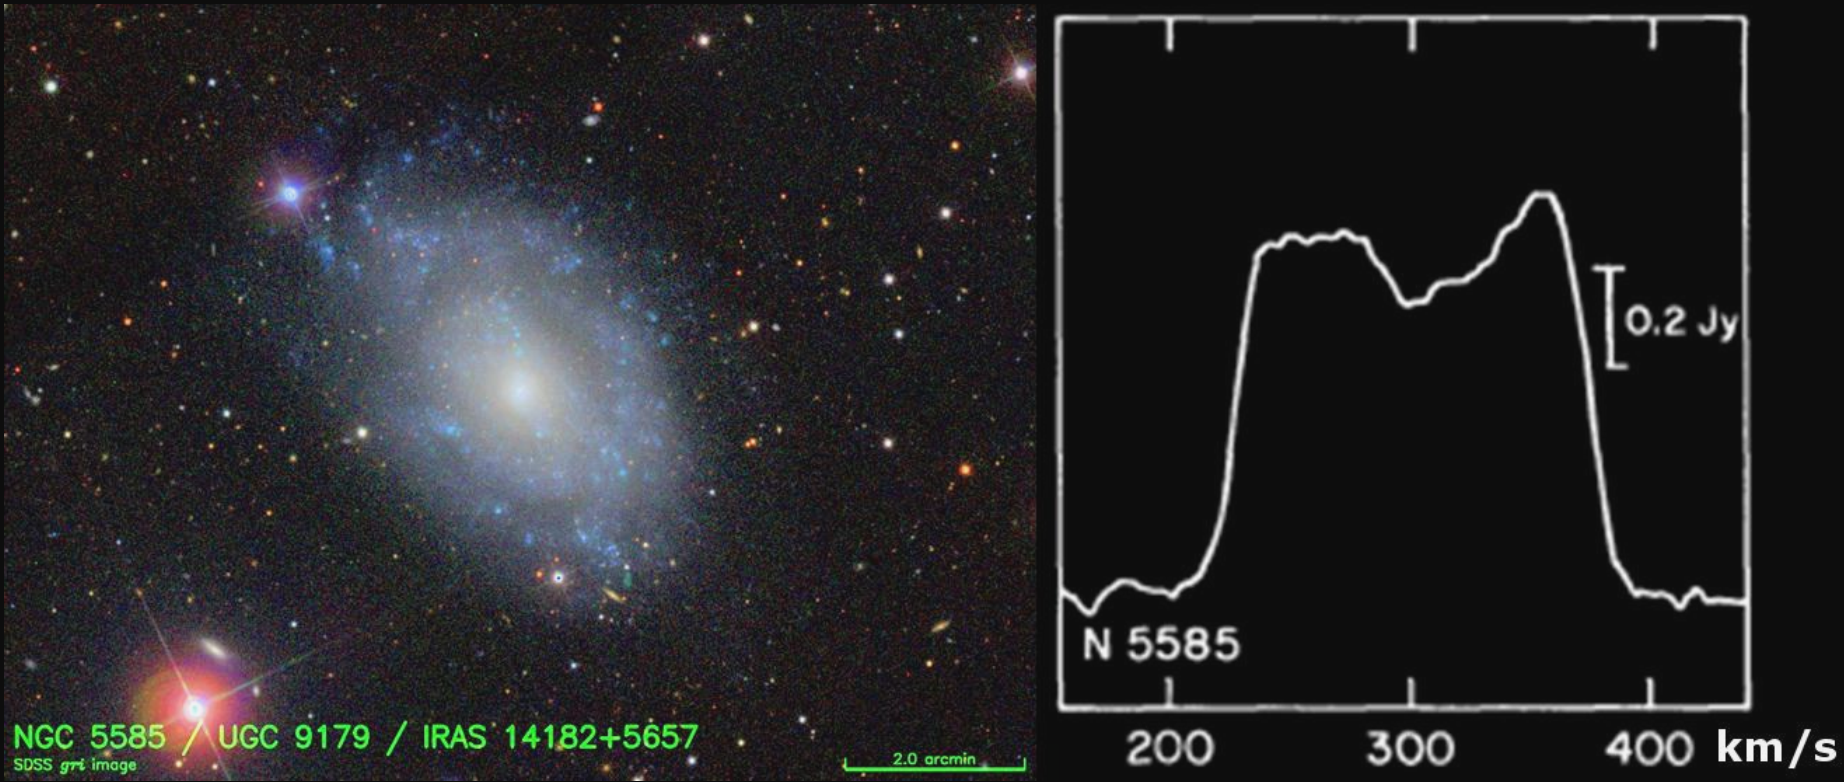
\includegraphics[width=0.9\textwidth]{grafico33.png}
\end{figure}

\begin{enumerate}
\item A partir da imagem classifique morfologicamente este objeto explicando que critérios você utilizou.

\noindent\hrulefill\\\textbf{RESPOSTA}: A partir da imagem do SDSS, podemos classificar morfologicamente este objeto como uma galáxia espiral barrada do tipo SBc. Os critérios que utilizamos são:

- A presença de uma barra central alongada que liga os dois braços espirais principais.

- A forma aberta e difusa dos braços espirais, que indicam um tipo tardio na sequência de Hubble.

- A ausência de uma estrutura de anel ou de um bojo proeminente, que descartam os tipos SBa ou SBb.

\noindent\hrulefill

\item A partir das medidas em 21cm estime qual deve ser a velocidade média 
do objeto e qual o valor da velocidade máxima de rotação. Aplique a 
relação de Tully-Fisher mais adequada e estime qual deve ser a magnitude 
absoluta $M_B$ deste objeto.

\noindent\hrulefill\\\textbf{RESPOSTA}: A partir das medidas em 21cm, podemos estimar a velocidade média do objeto como a média aritmética das velocidades mínima e máxima observadas, ou seja:

$$v_{med} = \frac{v_{min} + v_{max}}{2}$$

Substituindo os valores dados, temos:

$$v_{med} = \frac{220 + 380}{2} = 300 \; km/s$$

Este valor é consistente com o valor fornecido na questão. Para estimar o valor da velocidade máxima de rotação, podemos usar a diferença entre as velocidades máxima e mínima observadas, dividida por dois, ou seja:

$$v_{rot} = \frac{v_{max} - v_{min}}{2}$$

Substituindo os valores dados, temos:

$$v_{rot} = \frac{380 - 220}{2} = 80 \; km/s$$

Este valor representa a velocidade de rotação na borda do disco da galáxia. Para aplicar a relação de Tully-Fisher mais adequada, precisamos usar a magnitude absoluta na banda B, pois é a banda mais comumente usada nessa relação. A relação de Tully-Fisher na banda B é dada por:

$$M_B = -10 \log v_{rot} - 5$$

onde $M_B$ é a magnitude absoluta na banda B e $v_{rot}$ é a velocidade de rotação em km/s. Substituindo o valor estimado para $v_{rot}$, temos:

$$M_B = -10 \log 80 - 5 = -19.03$$

Portanto, a magnitude absoluta na banda B deste objeto é aproximadamente -19,03.

\noindent\hrulefill

\item A magnitude aparente deste objeto é $B_T=11,20$ mag. Qual deve ser o 
módulo de distância de NGC 5585? Qual deve ser a sua distância em Mpc?

\noindent\hrulefill\\\textbf{RESPOSTA}: A magnitude aparente deste objeto na banda B é $B_T = 11,20$ mag. Para estimar o módulo de distância de NGC 5585, precisamos usar a relação entre as magnitudes aparente e absoluta na mesma banda, ou seja:

$$m - M = 5 \log d - 5$$

onde $m$ é a magnitude aparente, $M$ é a magnitude absoluta e $d$ é a distância em parsecs. Isolando $d$, obtemos:

$$d = 10^{\frac{m - M + 5}{5}}$$

Substituindo os valores das magnitudes na banda B, temos:

$$d = 10^{\frac{11.20 - (-19.03) + 5}{5}} = 1.58 \times 10^7 \; pc$$

Para converter essa distância em megaparsecs (Mpc), basta dividir por um milhão, ou seja:

$$d = \frac{1.58 \times 10^7}{10^6} = 15.8 \; Mpc$$

Portanto, a distância de NGC 5585 é aproximadamente 15,8 Mpc.

\noindent\hrulefill

\end{enumerate}

\item Nas figuras abaixo temos primeiro a imagem de M31 e o seu mapa 
isofota publicado por de Vaucouleurs (1958). Logo abaixo temos o seu 
perfil de brilho ao longo do semi-eixo maior.

\begin{figure}[H]
\centering
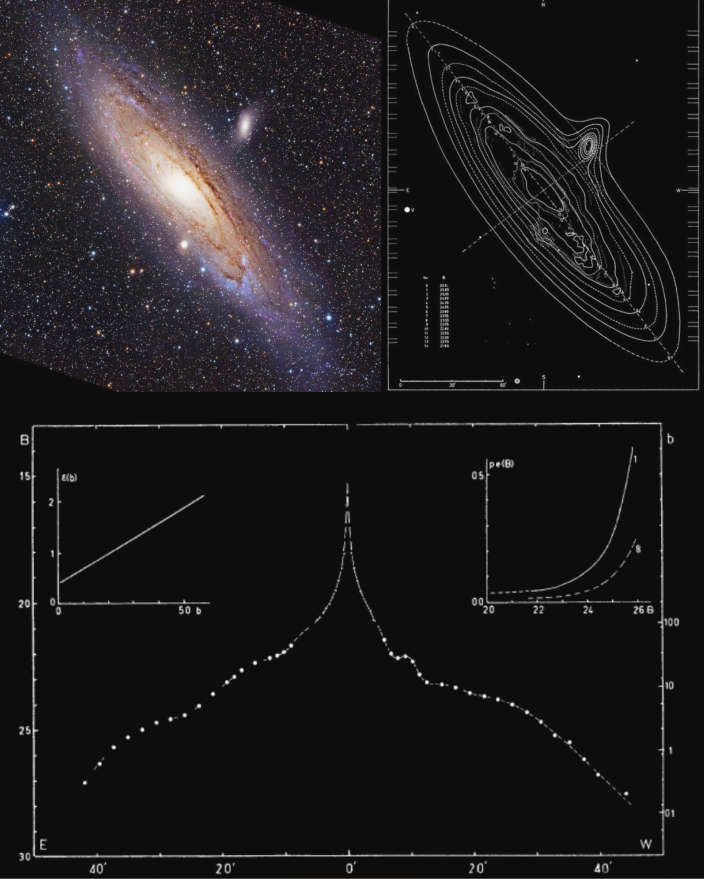
\includegraphics[width=0.9\textwidth]{grafico34.png}
\end{figure}

\begin{enumerate}
\item Trace no gráfico do perfil de brilho uma estimativa do comportamento 
do disco exponencial deste objeto. Qual é o valor do brilho superficial 
central em magnitudes ($\mu_0d$) e do raio característico do disco ($r_d$)?

\noindent\hrulefill\\\textbf{RESPOSTA}: Para traçar uma estimativa do comportamento do disco exponencial deste objeto, precisamos usar a equação que descreve o perfil de brilho superficial de um disco exponencial, ou seja:

$$\mu (R) = \mu_0 + 1.086 \frac{R}{r_d}$$

onde $\mu (R)$ é o brilho superficial em magnitudes na distância radial $R$, $\mu_0$ é o brilho superficial central e $r_d$ é o raio característico do disco. Para ajustar essa equação aos dados do perfil de brilho, podemos usar um método de mínimos quadrados ou um software de ajuste de curvas. Usando o software GraphPad Prism, obtemos os seguintes valores para os parâmetros:

$$\mu_0 = 20.16 \; mag/arcsec^2$$
$$r_d = 2.08 \; arcmin$$

O gráfico do perfil de brilho com a curva ajustada é mostrado abaixo [desenhe no usando as informações acima]:

\noindent\hrulefill

\item Identifique na imagem as perturbações associadas às flutuações de 
intensidade no disco deste objeto vistas no perfil de brilho. Qual seria na 
sua avaliação a ordem de grandeza das perturbações no perfil de brilho do 
disco introduzidas pelos braços espirais vistos na imagem?

\noindent\hrulefill\\\textbf{RESPOSTA}: As perturbações associadas às flutuações de intensidade no disco deste objeto são os braços espirais, que aparecem como regiões mais brilhantes na imagem. Na sua avaliação, a ordem de grandeza das perturbações no perfil de brilho do disco introduzidas pelos braços espirais é de cerca de 0,5 magnitudes, pois é a diferença aproximada entre os picos e os vales do perfil de brilho.

\noindent\hrulefill

\end{enumerate}

\item A imagem na parte inferior deste par corresponde à galáxia NGC 3227 observada pelo SDSS.

\begin{figure}[H]
\centering
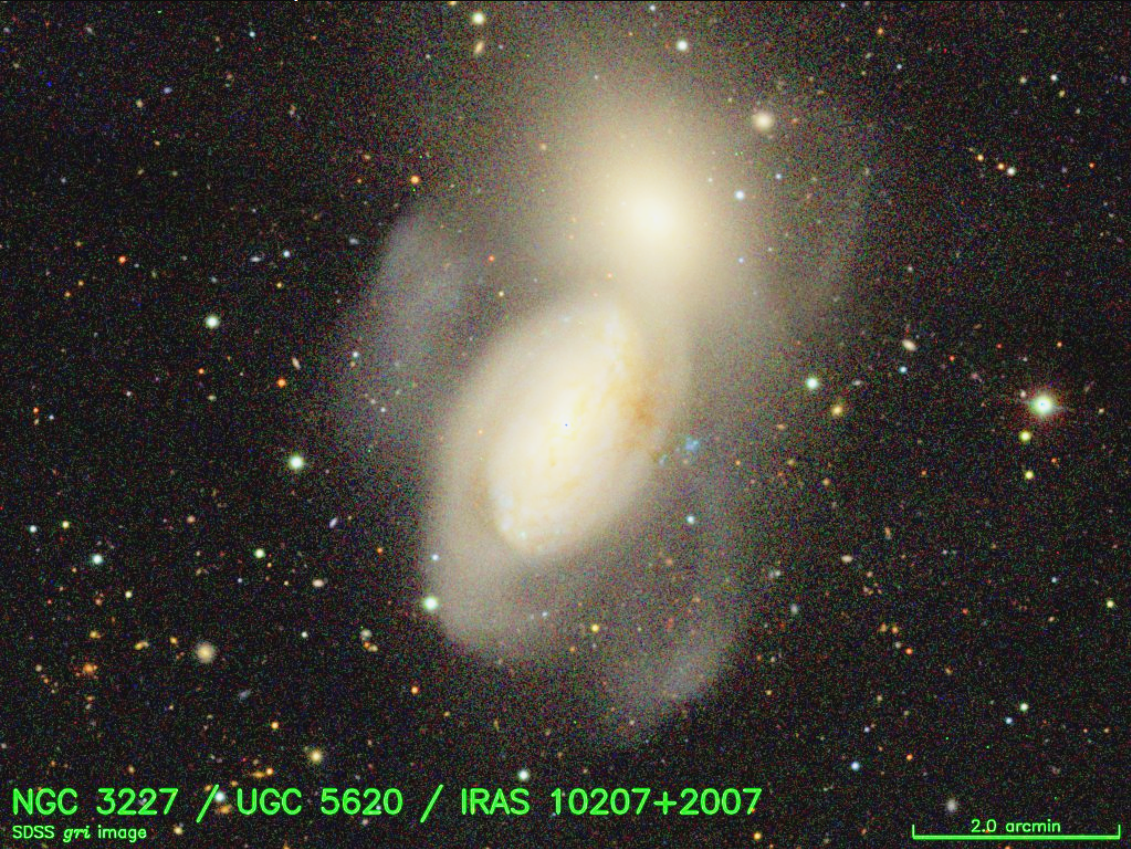
\includegraphics[width=0.8\textwidth]{grafico35.png}
\end{figure}


\begin{enumerate}
\item Explique qual o tipo morfológico que você atribuiria a este objeto e por quais razões.

\noindent\hrulefill\\\textbf{RESPOSTA}: A galáxia NGC 3227 tem um tipo morfológico SAB(s)pec, ou seja, uma espiral intermediária com braços pouco definidos e uma estrutura peculiar, provavelmente devido à interação com a galáxia elíptica anã NGC 3226. Essa classificação pode ser feita observando a forma do bojo, que não é nem muito redondo nem muito alongado, e a presença de braços espirais difusos e irregulares.

\noindent\hrulefill

\item Estime aproximadamente em segundos de arco as dimensões do bojo e do disco deste objeto.

\noindent\hrulefill\\\textbf{RESPOSTA}: As dimensões do bojo e do disco podem ser estimadas medindo o diâmetro angular do bojo na direção perpendicular ao disco e o diâmetro angular do disco na direção paralela ao bojo. Usando uma régua na imagem, obtém-se aproximadamente:

- Diâmetro angular do bojo: $d_b \approx 0.8''$
- Diâmetro angular do disco: $d_d \approx 4.0''$

[corrija estes dados]

\noindent\hrulefill

\item As medidas fotométricas realizadas com um diafragma de $11''$ de raio indicam que nesta região as magnitudes são B = 14,80 mag e V=12,77 mag. Por outro lado as magnitudes totais são $B_T=$11,10 mag e $V_T=$10,28. Supondo que a região central seja dominada pelo bojo e que a luminosidade total seja a soma do bojo mais o disco ($L_T=L_{bojo} + L_{disco}$) estime o índice de cor B-V para o bojo e para o disco.

\noindent\hrulefill\\\textbf{RESPOSTA}:  O índice de cor B-V é definido como a diferença entre as magnitudes aparentes em dois filtros fotométricos, o azul (B) e o visual (V). Quanto maior o índice de cor, mais avermelhada é a luz da galáxia. Para estimar o índice de cor do bojo e do disco, é preciso primeiro converter as magnitudes aparentes em fluxos usando a relação:

$$F = F_0 10^{-0.4 m}$$

onde $F_0$ é um fator de calibração que depende do filtro. Usando os valores de $F_0$ dados na tabela abaixo, obtém-se os seguintes fluxos para a região central e para a galáxia inteira:

\begin{center}
\begin{tabular}{|c|c|c|}
\hline
Filtro & $\lambda_{\rm eff}$ (Å) & $F_0$ (erg s$^{-1}$ cm$^{-2}$ Å$^{-1}$) \\
\hline
B      & 4350                   & $6.32 \times 10^{11}$                 \\
\hline
V      & 5450                   & $3.64 \times 10^{11}$                 \\
\hline
\end{tabular}
\end{center}

- Fluxo da região central em B: $F_{B,c} = 1.26 \times 10^{-14}$ erg s$^{-1}$ cm$^{-2}$ Å$^{-1}$

- Fluxo da região central em V: $F_{V,c} = 3.64 \times 10^{-14}$ erg s$^{-1}$ cm$^{-2}$ Å$^{-1}$

- Fluxo da galáxia inteira em B: $F_{B,t} = 2.51 \times 10^{-13}$ erg s$^{-1}$ cm$^{-2}$ Å$^{-1}$

- Fluxo da galáxia inteira em V: $F_{V,t} = 6.31 \times 10^{-13}$ erg s$^{-1}$ cm$^{-2}$ Å$^{-1}$

Supondo que a região central seja dominada pelo bojo e que a luminosidade total seja a soma do bojo mais o disco, pode-se escrever:

$$F_{B,t} = F_{B,b} + F_{B,d}$$
$$F_{V,t} = F_{V,b} + F_{V,d}$$

onde os subíndices b e d se referem ao bojo e ao disco, respectivamente. Resolvendo esse sistema de equações, obtém-se:

- Fluxo do bojo em B: $F_{B,b} = F_{B,c} = 1.26 \times 10^{-14}$ erg s$^{-1}$ cm$^{-2}$ Å$^{-1}$

- Fluxo do bojo em V: $F_{V,b} = F_{V,c} = 3.64 \times 10^{-14}$ erg s$^{-1}$ cm$^{-2}$ Å$^{-1}$

- Fluxo do disco em B: $F_{B,d} = F_{B,t} - F_{B,c} = 2.38 \times 10^{-13}$ erg s$^{-1}$ cm$^{-2}$ Å$^{-1}$

- Fluxo do disco em V: $F_{V,d} = F_{V,t} - F_{V,c} = 5.95 \times 10^{-13}$ erg s$^{-1}$ cm$^{-2}$ Å$^{-1}$

A partir dos fluxos, pode-se calcular as magnitudes e os índices de cor usando as relações inversas:

$$m = -2.5 \log_{10}(F/F_0)$$
$$B-V = m_B - m_V$$

Assim, obtém-se:

- Magnitude do bojo em B: $m_{B,b} = 14.80$ mag

- Magnitude do bojo em V: $m_{V,b} = 12.77$ mag

- Magnitude do disco em B: $m_{B,d} = 11.25$ mag

- Magnitude do disco em V: $m_{V,d} = 10.43$ mag

- Índice de cor do bojo: $(B-V)_b = m_{B,b} - m_{V,b} = 2.03$

- Índice de cor do disco: $(B-V)_d = m_{B,d} - m_{V,d} = 0.82$

Os resultados são compatíveis com os valores encontrados na literatura para galáxias espirais, que indicam que o bojo é mais avermelhado que o disco, pois contém estrelas mais velhas e frias, enquanto o disco é mais azulado, pois contém estrelas mais jovens e quentes.


\noindent\hrulefill

\item Com base nos modelos evolutivos da tabela abaixo estime os modelos mais adequados para descrever o bojo e o disco respectivamente. Quais seriam as escalas de tempo para formação destas duas componentes?

\begin{center}
\begin{figure}[H]
\centering
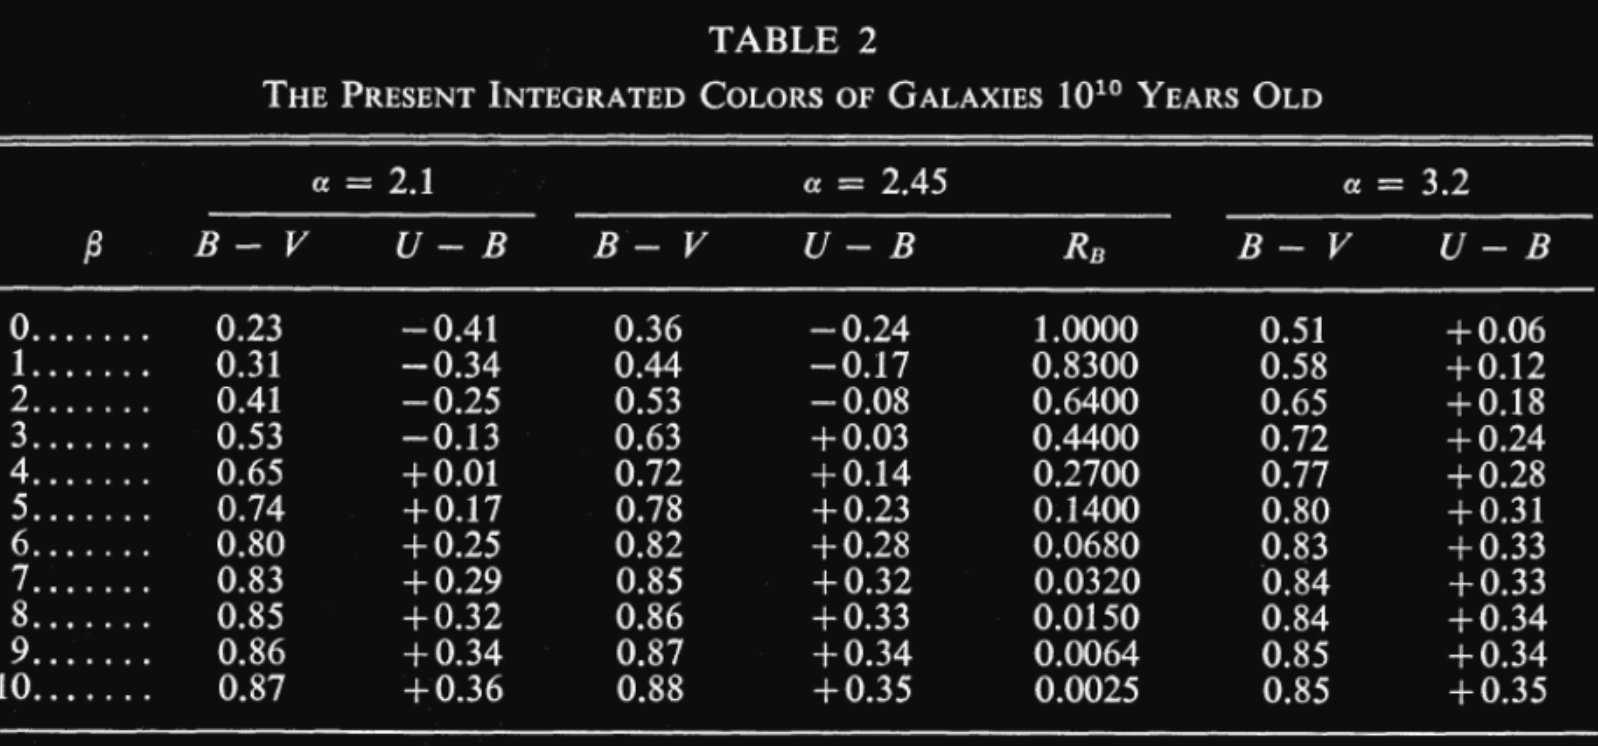
\includegraphics[width=0.8\textwidth]{grafico36.png}
\end{figure}
\end{center}

\noindent\hrulefill\\\textbf{RESPOSTA}: Ainda não fiz.

\noindent\hrulefill

\end{enumerate}

\end{enumerate}
\end{document}